% Options for packages loaded elsewhere
\PassOptionsToPackage{unicode}{hyperref}
\PassOptionsToPackage{hyphens}{url}
%
\documentclass[
]{article}
\usepackage{lmodern}
\usepackage{amssymb,amsmath}
\usepackage{ifxetex,ifluatex}
\ifnum 0\ifxetex 1\fi\ifluatex 1\fi=0 % if pdftex
  \usepackage[T1]{fontenc}
  \usepackage[utf8]{inputenc}
  \usepackage{textcomp} % provide euro and other symbols
\else % if luatex or xetex
  \usepackage{unicode-math}
  \defaultfontfeatures{Scale=MatchLowercase}
  \defaultfontfeatures[\rmfamily]{Ligatures=TeX,Scale=1}
\fi
% Use upquote if available, for straight quotes in verbatim environments
\IfFileExists{upquote.sty}{\usepackage{upquote}}{}
\IfFileExists{microtype.sty}{% use microtype if available
  \usepackage[]{microtype}
  \UseMicrotypeSet[protrusion]{basicmath} % disable protrusion for tt fonts
}{}
\makeatletter
\@ifundefined{KOMAClassName}{% if non-KOMA class
  \IfFileExists{parskip.sty}{%
    \usepackage{parskip}
  }{% else
    \setlength{\parindent}{0pt}
    \setlength{\parskip}{6pt plus 2pt minus 1pt}}
}{% if KOMA class
  \KOMAoptions{parskip=half}}
\makeatother
\usepackage{xcolor}
\IfFileExists{xurl.sty}{\usepackage{xurl}}{} % add URL line breaks if available
\IfFileExists{bookmark.sty}{\usepackage{bookmark}}{\usepackage{hyperref}}
\hypersetup{
  pdftitle={Analysis 2: Supplemental Analysis with Original and Mail-In Data (Movers)},
  pdfauthor={Fan Lu \& Gento Kato},
  hidelinks,
  pdfcreator={LaTeX via pandoc}}
\urlstyle{same} % disable monospaced font for URLs
\usepackage[margin=1in]{geometry}
\usepackage{color}
\usepackage{fancyvrb}
\newcommand{\VerbBar}{|}
\newcommand{\VERB}{\Verb[commandchars=\\\{\}]}
\DefineVerbatimEnvironment{Highlighting}{Verbatim}{commandchars=\\\{\}}
% Add ',fontsize=\small' for more characters per line
\usepackage{framed}
\definecolor{shadecolor}{RGB}{248,248,248}
\newenvironment{Shaded}{\begin{snugshade}}{\end{snugshade}}
\newcommand{\AlertTok}[1]{\textcolor[rgb]{0.94,0.16,0.16}{#1}}
\newcommand{\AnnotationTok}[1]{\textcolor[rgb]{0.56,0.35,0.01}{\textbf{\textit{#1}}}}
\newcommand{\AttributeTok}[1]{\textcolor[rgb]{0.77,0.63,0.00}{#1}}
\newcommand{\BaseNTok}[1]{\textcolor[rgb]{0.00,0.00,0.81}{#1}}
\newcommand{\BuiltInTok}[1]{#1}
\newcommand{\CharTok}[1]{\textcolor[rgb]{0.31,0.60,0.02}{#1}}
\newcommand{\CommentTok}[1]{\textcolor[rgb]{0.56,0.35,0.01}{\textit{#1}}}
\newcommand{\CommentVarTok}[1]{\textcolor[rgb]{0.56,0.35,0.01}{\textbf{\textit{#1}}}}
\newcommand{\ConstantTok}[1]{\textcolor[rgb]{0.00,0.00,0.00}{#1}}
\newcommand{\ControlFlowTok}[1]{\textcolor[rgb]{0.13,0.29,0.53}{\textbf{#1}}}
\newcommand{\DataTypeTok}[1]{\textcolor[rgb]{0.13,0.29,0.53}{#1}}
\newcommand{\DecValTok}[1]{\textcolor[rgb]{0.00,0.00,0.81}{#1}}
\newcommand{\DocumentationTok}[1]{\textcolor[rgb]{0.56,0.35,0.01}{\textbf{\textit{#1}}}}
\newcommand{\ErrorTok}[1]{\textcolor[rgb]{0.64,0.00,0.00}{\textbf{#1}}}
\newcommand{\ExtensionTok}[1]{#1}
\newcommand{\FloatTok}[1]{\textcolor[rgb]{0.00,0.00,0.81}{#1}}
\newcommand{\FunctionTok}[1]{\textcolor[rgb]{0.00,0.00,0.00}{#1}}
\newcommand{\ImportTok}[1]{#1}
\newcommand{\InformationTok}[1]{\textcolor[rgb]{0.56,0.35,0.01}{\textbf{\textit{#1}}}}
\newcommand{\KeywordTok}[1]{\textcolor[rgb]{0.13,0.29,0.53}{\textbf{#1}}}
\newcommand{\NormalTok}[1]{#1}
\newcommand{\OperatorTok}[1]{\textcolor[rgb]{0.81,0.36,0.00}{\textbf{#1}}}
\newcommand{\OtherTok}[1]{\textcolor[rgb]{0.56,0.35,0.01}{#1}}
\newcommand{\PreprocessorTok}[1]{\textcolor[rgb]{0.56,0.35,0.01}{\textit{#1}}}
\newcommand{\RegionMarkerTok}[1]{#1}
\newcommand{\SpecialCharTok}[1]{\textcolor[rgb]{0.00,0.00,0.00}{#1}}
\newcommand{\SpecialStringTok}[1]{\textcolor[rgb]{0.31,0.60,0.02}{#1}}
\newcommand{\StringTok}[1]{\textcolor[rgb]{0.31,0.60,0.02}{#1}}
\newcommand{\VariableTok}[1]{\textcolor[rgb]{0.00,0.00,0.00}{#1}}
\newcommand{\VerbatimStringTok}[1]{\textcolor[rgb]{0.31,0.60,0.02}{#1}}
\newcommand{\WarningTok}[1]{\textcolor[rgb]{0.56,0.35,0.01}{\textbf{\textit{#1}}}}
\usepackage{graphicx,grffile}
\makeatletter
\def\maxwidth{\ifdim\Gin@nat@width>\linewidth\linewidth\else\Gin@nat@width\fi}
\def\maxheight{\ifdim\Gin@nat@height>\textheight\textheight\else\Gin@nat@height\fi}
\makeatother
% Scale images if necessary, so that they will not overflow the page
% margins by default, and it is still possible to overwrite the defaults
% using explicit options in \includegraphics[width, height, ...]{}
\setkeys{Gin}{width=\maxwidth,height=\maxheight,keepaspectratio}
% Set default figure placement to htbp
\makeatletter
\def\fps@figure{htbp}
\makeatother
\setlength{\emergencystretch}{3em} % prevent overfull lines
\providecommand{\tightlist}{%
  \setlength{\itemsep}{0pt}\setlength{\parskip}{0pt}}
\setcounter{secnumdepth}{-\maxdimen} % remove section numbering
\usepackage{bookmark}
\usepackage{xltxtra}
\usepackage{zxjatype}
\usepackage[ipa]{zxjafont}

\title{Analysis 2: Supplemental Analysis with Original and Mail-In Data
(Movers)}
\author{Fan Lu \& Gento Kato}
\date{January 26, 2021}

\begin{document}
\maketitle

\hypertarget{analytical-strategy}{%
\section{Analytical Strategy}\label{analytical-strategy}}

\hypertarget{variables}{%
\subsection{Variables}\label{variables}}

\begin{itemize}
\item
  Outcome: Foreigner Suffrage (min 0, max 1)
\item
  Mediator 1: (Objective) Political Knowledge (min = 0, max = 1)
\item
  Mediator 2: Ideology (min 0 = left/liberal, max 1 =
  right/conservative)
\item
  Mediator 3: LDP - DPJ FT (min 0 = favor DPJ, max 1 = favor LDP)
\item
  Mediator 4: Favorability of South Korea (min = 0, max = 1)\\
\item
  Mediator 5: Favorability of China (min = 0, max = 1)\\
\item
  Mediator 6: Favorability of USA (min = 0, max = 1)\\
\item
  Mediator 7: Income (percentile, min = 0, max = 1)
\item
  Independent Variable: University Education (0 = Junior College or
  Less, 1 = University or More)
\item
  Moderator 1: Gender (0 = Female, 1 = Male), This means that all
  ``base'' coefficients are for female.
\item
  Moderator 2: Age (by 10 years, centered at 20). Reasoning: Two trends
  may influence the role of university education. (1) There is an
  evident increase in number of university graduates over the years,
  especially among women. This trend may impies that university
  experience may be more gendered in the past than today. (2) There is a
  trend of ``internationalization'' in university education in recent
  days. Therefore, the diversifying and liberalizing effect of education
  may be stronger for younger generation.
\item
  Control 1: Percent in life residing locally. More locally-identified
  individuals may dislike outsiders more.
\item
  Control 2: (ZIP level) Residing in densely inhabited district (DID)
\item
  Control 3: (ZIP level) Percent of foreigners in neighborhood
  (transformed by square root)\\
\item
  Control 4: (ZIP level) Percent of university graduates in neighborhood
  (by 10 percent)
\item
  Control 5: (Municipality level) Percent of residents residing in DID
\item
  Control 6: (Municipality level) Percent of foreigners (transformed by
  square root)
\item
  Control 7: (Municipality level) Percent of university graduates (by 10
  percent)
\end{itemize}

\hypertarget{subset-data}{%
\subsection{Subset Data}\label{subset-data}}

Analysis is conducted on the following subset.

If age - years of local ZIP residence is 23 or larger. 23 is the age of
graduating university (the youngest possible) in Japan. Assuming that an
individual is living in the local ZIP continuously, this condition
implies that one moved to the ZIP of current residence (likely) after
graduating the university. This incorporates the possibility that
education changes attitudes through the movement in residence.

\hypertarget{modeling-strategy}{%
\subsection{Modeling Strategy}\label{modeling-strategy}}

All models are estimated by OLS. For outcome model, alternative model is
estimated by the multinomial logit model, with 3 category DV (disagree,
neither, agree), with disagree as a reference category.

\hypertarget{robustness-check-in-this-file}{%
\subsection{Robustness Check (in this
file)}\label{robustness-check-in-this-file}}

SIFCCT has one special survey where they conducted a survey through
mail. Mail survey contains identical set of variables as online survey.
So I replicated the analysis with the mail survey.

\hypertarget{preparation}{%
\section{Preparation}\label{preparation}}

\begin{Shaded}
\begin{Highlighting}[]
\CommentTok{## Clean Up Space}
\KeywordTok{rm}\NormalTok{(}\DataTypeTok{list=}\KeywordTok{ls}\NormalTok{())}

\CommentTok{## Set Working Directory (Automatically) ##}
\KeywordTok{require}\NormalTok{(rstudioapi); }\KeywordTok{require}\NormalTok{(rprojroot)}
\ControlFlowTok{if}\NormalTok{ (rstudioapi}\OperatorTok{::}\KeywordTok{isAvailable}\NormalTok{()}\OperatorTok{==}\OtherTok{TRUE}\NormalTok{) \{}
  \KeywordTok{setwd}\NormalTok{(}\KeywordTok{dirname}\NormalTok{(rstudioapi}\OperatorTok{::}\KeywordTok{getActiveDocumentContext}\NormalTok{()}\OperatorTok{$}\NormalTok{path)); }
\NormalTok{\} }
\NormalTok{projdir <-}\StringTok{ }\KeywordTok{find_root}\NormalTok{(}\KeywordTok{has_file}\NormalTok{(}\StringTok{"thisishome.txt"}\NormalTok{))}
\KeywordTok{cat}\NormalTok{(}\KeywordTok{paste}\NormalTok{(}\StringTok{"Working Directory Set to:}\CharTok{\textbackslash{}n}\StringTok{"}\NormalTok{,projdir))}
\end{Highlighting}
\end{Shaded}

\begin{verbatim}
## Working Directory Set to:
##  /home/gentok/GoogleDrive/Projects/Fan-Gento-Lab/ForeignerJapan
\end{verbatim}

\begin{Shaded}
\begin{Highlighting}[]
\KeywordTok{setwd}\NormalTok{(projdir)}

\CommentTok{## Original Data}
\NormalTok{datadir1a <-}\StringTok{ }\KeywordTok{paste0}\NormalTok{(projdir, }\StringTok{"/data/sifcct_zip_latest_v5.rds"}\NormalTok{)}
\NormalTok{datadir1b <-}\StringTok{ }\KeywordTok{paste0}\NormalTok{(projdir, }\StringTok{"/data/sifcct_zip_latest_panel_v5.rds"}\NormalTok{)}
\NormalTok{datadir2 <-}\StringTok{ }\KeywordTok{paste0}\NormalTok{(projdir, }\StringTok{"/data/mail_zip_latest_v5.rds"}\NormalTok{)}

\CommentTok{## packages}
\CommentTok{# devtools::install_github("gentok/estvis")}
\CommentTok{# require(estvis)}
\KeywordTok{require}\NormalTok{(multiwayvcov)}
\KeywordTok{require}\NormalTok{(sandwich)}
\KeywordTok{require}\NormalTok{(lmtest)}
\KeywordTok{require}\NormalTok{(MASS)}
\CommentTok{# devtools::install_github("tidyverse/ggplot2") # Need development version (as of Dec 31, 2019)}
\KeywordTok{library}\NormalTok{(ggplot2)}
\KeywordTok{require}\NormalTok{(texreg)}
\CommentTok{# require(brant)}
\CommentTok{# require(VGAM)}
\CommentTok{# require(nnet)}
\KeywordTok{require}\NormalTok{(mlogit)}
\KeywordTok{require}\NormalTok{(Formula)}
\end{Highlighting}
\end{Shaded}

\hypertarget{import-and-clean-data}{%
\section{Import and clean data}\label{import-and-clean-data}}

\begin{Shaded}
\begin{Highlighting}[]
\CommentTok{###################}
\CommentTok{## SIFCCT Online ##}
\CommentTok{###################}

\NormalTok{sifcct <-}\StringTok{ }\KeywordTok{rbind}\NormalTok{(}\KeywordTok{readRDS}\NormalTok{(datadir1a),}\KeywordTok{readRDS}\NormalTok{(datadir1b))}

\CommentTok{## Knowledge Variable (Replaced)}
\NormalTok{sifcct}\OperatorTok{$}\NormalTok{knowledge[sifcct}\OperatorTok{$}\NormalTok{panel}\OperatorTok{==}\DecValTok{1} \OperatorTok{&}\StringTok{ }\NormalTok{sifcct}\OperatorTok{$}\NormalTok{wave}\OperatorTok{==}\DecValTok{2}\NormalTok{] <-}\StringTok{ }\NormalTok{sifcct}\OperatorTok{$}\NormalTok{knowledge[sifcct}\OperatorTok{$}\NormalTok{panel}\OperatorTok{==}\DecValTok{1} \OperatorTok{&}\StringTok{ }\NormalTok{sifcct}\OperatorTok{$}\NormalTok{wave}\OperatorTok{==}\DecValTok{1}\NormalTok{][}\KeywordTok{match}\NormalTok{(sifcct}\OperatorTok{$}\NormalTok{panelid[sifcct}\OperatorTok{$}\NormalTok{panel}\OperatorTok{==}\DecValTok{1} \OperatorTok{&}\StringTok{ }\NormalTok{sifcct}\OperatorTok{$}\NormalTok{wave}\OperatorTok{==}\DecValTok{2}\NormalTok{],sifcct}\OperatorTok{$}\NormalTok{panelid[sifcct}\OperatorTok{$}\NormalTok{panel}\OperatorTok{==}\DecValTok{1} \OperatorTok{&}\StringTok{ }\NormalTok{sifcct}\OperatorTok{$}\NormalTok{wave}\OperatorTok{==}\DecValTok{1}\NormalTok{])]}
\NormalTok{sifcct}\OperatorTok{$}\NormalTok{knowledge[sifcct}\OperatorTok{$}\NormalTok{panel}\OperatorTok{==}\DecValTok{1} \OperatorTok{&}\StringTok{ }\NormalTok{sifcct}\OperatorTok{$}\NormalTok{wave}\OperatorTok{==}\DecValTok{3}\NormalTok{] <-}\StringTok{ }\NormalTok{sifcct}\OperatorTok{$}\NormalTok{knowledge[sifcct}\OperatorTok{$}\NormalTok{panel}\OperatorTok{==}\DecValTok{1} \OperatorTok{&}\StringTok{ }\NormalTok{sifcct}\OperatorTok{$}\NormalTok{wave}\OperatorTok{==}\DecValTok{1}\NormalTok{][}\KeywordTok{match}\NormalTok{(sifcct}\OperatorTok{$}\NormalTok{panelid[sifcct}\OperatorTok{$}\NormalTok{panel}\OperatorTok{==}\DecValTok{1} \OperatorTok{&}\StringTok{ }\NormalTok{sifcct}\OperatorTok{$}\NormalTok{wave}\OperatorTok{==}\DecValTok{3}\NormalTok{],sifcct}\OperatorTok{$}\NormalTok{panelid[sifcct}\OperatorTok{$}\NormalTok{panel}\OperatorTok{==}\DecValTok{1} \OperatorTok{&}\StringTok{ }\NormalTok{sifcct}\OperatorTok{$}\NormalTok{wave}\OperatorTok{==}\DecValTok{1}\NormalTok{])]}
\NormalTok{sifcct}\OperatorTok{$}\NormalTok{knowledge[sifcct}\OperatorTok{$}\NormalTok{panel}\OperatorTok{==}\DecValTok{1} \OperatorTok{&}\StringTok{ }\NormalTok{sifcct}\OperatorTok{$}\NormalTok{wave}\OperatorTok{==}\DecValTok{4}\NormalTok{] <-}\StringTok{ }\NormalTok{sifcct}\OperatorTok{$}\NormalTok{knowledge[sifcct}\OperatorTok{$}\NormalTok{panel}\OperatorTok{==}\DecValTok{1} \OperatorTok{&}\StringTok{ }\NormalTok{sifcct}\OperatorTok{$}\NormalTok{wave}\OperatorTok{==}\DecValTok{1}\NormalTok{][}\KeywordTok{match}\NormalTok{(sifcct}\OperatorTok{$}\NormalTok{panelid[sifcct}\OperatorTok{$}\NormalTok{panel}\OperatorTok{==}\DecValTok{1} \OperatorTok{&}\StringTok{ }\NormalTok{sifcct}\OperatorTok{$}\NormalTok{wave}\OperatorTok{==}\DecValTok{4}\NormalTok{],sifcct}\OperatorTok{$}\NormalTok{panelid[sifcct}\OperatorTok{$}\NormalTok{panel}\OperatorTok{==}\DecValTok{1} \OperatorTok{&}\StringTok{ }\NormalTok{sifcct}\OperatorTok{$}\NormalTok{wave}\OperatorTok{==}\DecValTok{1}\NormalTok{])]}
\NormalTok{sifcct}\OperatorTok{$}\NormalTok{knowledge[sifcct}\OperatorTok{$}\NormalTok{panel}\OperatorTok{==}\DecValTok{1} \OperatorTok{&}\StringTok{ }\NormalTok{sifcct}\OperatorTok{$}\NormalTok{wave}\OperatorTok{==}\DecValTok{5}\NormalTok{] <-}\StringTok{ }\NormalTok{sifcct}\OperatorTok{$}\NormalTok{knowledge[sifcct}\OperatorTok{$}\NormalTok{panel}\OperatorTok{==}\DecValTok{1} \OperatorTok{&}\StringTok{ }\NormalTok{sifcct}\OperatorTok{$}\NormalTok{wave}\OperatorTok{==}\DecValTok{1}\NormalTok{][}\KeywordTok{match}\NormalTok{(sifcct}\OperatorTok{$}\NormalTok{panelid[sifcct}\OperatorTok{$}\NormalTok{panel}\OperatorTok{==}\DecValTok{1} \OperatorTok{&}\StringTok{ }\NormalTok{sifcct}\OperatorTok{$}\NormalTok{wave}\OperatorTok{==}\DecValTok{5}\NormalTok{],sifcct}\OperatorTok{$}\NormalTok{panelid[sifcct}\OperatorTok{$}\NormalTok{panel}\OperatorTok{==}\DecValTok{1} \OperatorTok{&}\StringTok{ }\NormalTok{sifcct}\OperatorTok{$}\NormalTok{wave}\OperatorTok{==}\DecValTok{1}\NormalTok{])]}
\NormalTok{sifcct}\OperatorTok{$}\NormalTok{knowledge[sifcct}\OperatorTok{$}\NormalTok{panel}\OperatorTok{==}\DecValTok{1} \OperatorTok{&}\StringTok{ }\NormalTok{sifcct}\OperatorTok{$}\NormalTok{wave}\OperatorTok{==}\DecValTok{6}\NormalTok{] <-}\StringTok{ }\NormalTok{sifcct}\OperatorTok{$}\NormalTok{knowledge[sifcct}\OperatorTok{$}\NormalTok{panel}\OperatorTok{==}\DecValTok{1} \OperatorTok{&}\StringTok{ }\NormalTok{sifcct}\OperatorTok{$}\NormalTok{wave}\OperatorTok{==}\DecValTok{1}\NormalTok{][}\KeywordTok{match}\NormalTok{(sifcct}\OperatorTok{$}\NormalTok{panelid[sifcct}\OperatorTok{$}\NormalTok{panel}\OperatorTok{==}\DecValTok{1} \OperatorTok{&}\StringTok{ }\NormalTok{sifcct}\OperatorTok{$}\NormalTok{wave}\OperatorTok{==}\DecValTok{6}\NormalTok{],sifcct}\OperatorTok{$}\NormalTok{panelid[sifcct}\OperatorTok{$}\NormalTok{panel}\OperatorTok{==}\DecValTok{1} \OperatorTok{&}\StringTok{ }\NormalTok{sifcct}\OperatorTok{$}\NormalTok{wave}\OperatorTok{==}\DecValTok{1}\NormalTok{])]}
\NormalTok{sifcct}\OperatorTok{$}\NormalTok{knowledge[sifcct}\OperatorTok{$}\NormalTok{panel}\OperatorTok{==}\DecValTok{1} \OperatorTok{&}\StringTok{ }\NormalTok{sifcct}\OperatorTok{$}\NormalTok{wave}\OperatorTok{==}\DecValTok{7}\NormalTok{] <-}\StringTok{ }\NormalTok{sifcct}\OperatorTok{$}\NormalTok{knowledge[sifcct}\OperatorTok{$}\NormalTok{panel}\OperatorTok{==}\DecValTok{1} \OperatorTok{&}\StringTok{ }\NormalTok{sifcct}\OperatorTok{$}\NormalTok{wave}\OperatorTok{==}\DecValTok{1}\NormalTok{][}\KeywordTok{match}\NormalTok{(sifcct}\OperatorTok{$}\NormalTok{panelid[sifcct}\OperatorTok{$}\NormalTok{panel}\OperatorTok{==}\DecValTok{1} \OperatorTok{&}\StringTok{ }\NormalTok{sifcct}\OperatorTok{$}\NormalTok{wave}\OperatorTok{==}\DecValTok{7}\NormalTok{],sifcct}\OperatorTok{$}\NormalTok{panelid[sifcct}\OperatorTok{$}\NormalTok{panel}\OperatorTok{==}\DecValTok{1} \OperatorTok{&}\StringTok{ }\NormalTok{sifcct}\OperatorTok{$}\NormalTok{wave}\OperatorTok{==}\DecValTok{1}\NormalTok{])]}
\NormalTok{sifcct}\OperatorTok{$}\NormalTok{knowledge[sifcct}\OperatorTok{$}\NormalTok{panel}\OperatorTok{==}\DecValTok{1} \OperatorTok{&}\StringTok{ }\NormalTok{sifcct}\OperatorTok{$}\NormalTok{wave}\OperatorTok{==}\DecValTok{8}\NormalTok{] <-}\StringTok{ }\NormalTok{sifcct}\OperatorTok{$}\NormalTok{knowledge[sifcct}\OperatorTok{$}\NormalTok{panel}\OperatorTok{==}\DecValTok{1} \OperatorTok{&}\StringTok{ }\NormalTok{sifcct}\OperatorTok{$}\NormalTok{wave}\OperatorTok{==}\DecValTok{1}\NormalTok{][}\KeywordTok{match}\NormalTok{(sifcct}\OperatorTok{$}\NormalTok{panelid[sifcct}\OperatorTok{$}\NormalTok{panel}\OperatorTok{==}\DecValTok{1} \OperatorTok{&}\StringTok{ }\NormalTok{sifcct}\OperatorTok{$}\NormalTok{wave}\OperatorTok{==}\DecValTok{8}\NormalTok{],sifcct}\OperatorTok{$}\NormalTok{panelid[sifcct}\OperatorTok{$}\NormalTok{panel}\OperatorTok{==}\DecValTok{1} \OperatorTok{&}\StringTok{ }\NormalTok{sifcct}\OperatorTok{$}\NormalTok{wave}\OperatorTok{==}\DecValTok{1}\NormalTok{])]}
\NormalTok{sifcct}\OperatorTok{$}\NormalTok{knowledge[sifcct}\OperatorTok{$}\NormalTok{panel}\OperatorTok{==}\DecValTok{1} \OperatorTok{&}\StringTok{ }\NormalTok{sifcct}\OperatorTok{$}\NormalTok{wave}\OperatorTok{==}\DecValTok{9}\NormalTok{] <-}\StringTok{ }\NormalTok{sifcct}\OperatorTok{$}\NormalTok{knowledge[sifcct}\OperatorTok{$}\NormalTok{panel}\OperatorTok{==}\DecValTok{1} \OperatorTok{&}\StringTok{ }\NormalTok{sifcct}\OperatorTok{$}\NormalTok{wave}\OperatorTok{==}\DecValTok{1}\NormalTok{][}\KeywordTok{match}\NormalTok{(sifcct}\OperatorTok{$}\NormalTok{panelid[sifcct}\OperatorTok{$}\NormalTok{panel}\OperatorTok{==}\DecValTok{1} \OperatorTok{&}\StringTok{ }\NormalTok{sifcct}\OperatorTok{$}\NormalTok{wave}\OperatorTok{==}\DecValTok{9}\NormalTok{],sifcct}\OperatorTok{$}\NormalTok{panelid[sifcct}\OperatorTok{$}\NormalTok{panel}\OperatorTok{==}\DecValTok{1} \OperatorTok{&}\StringTok{ }\NormalTok{sifcct}\OperatorTok{$}\NormalTok{wave}\OperatorTok{==}\DecValTok{1}\NormalTok{])]}
\NormalTok{sifcct}\OperatorTok{$}\NormalTok{knowledge[sifcct}\OperatorTok{$}\NormalTok{panel}\OperatorTok{==}\DecValTok{1} \OperatorTok{&}\StringTok{ }\NormalTok{sifcct}\OperatorTok{$}\NormalTok{wave}\OperatorTok{==}\DecValTok{10}\NormalTok{] <-}\StringTok{ }\NormalTok{sifcct}\OperatorTok{$}\NormalTok{knowledge[sifcct}\OperatorTok{$}\NormalTok{panel}\OperatorTok{==}\DecValTok{1} \OperatorTok{&}\StringTok{ }\NormalTok{sifcct}\OperatorTok{$}\NormalTok{wave}\OperatorTok{==}\DecValTok{1}\NormalTok{][}\KeywordTok{match}\NormalTok{(sifcct}\OperatorTok{$}\NormalTok{panelid[sifcct}\OperatorTok{$}\NormalTok{panel}\OperatorTok{==}\DecValTok{1} \OperatorTok{&}\StringTok{ }\NormalTok{sifcct}\OperatorTok{$}\NormalTok{wave}\OperatorTok{==}\DecValTok{10}\NormalTok{],sifcct}\OperatorTok{$}\NormalTok{panelid[sifcct}\OperatorTok{$}\NormalTok{panel}\OperatorTok{==}\DecValTok{1} \OperatorTok{&}\StringTok{ }\NormalTok{sifcct}\OperatorTok{$}\NormalTok{wave}\OperatorTok{==}\DecValTok{1}\NormalTok{])]}
\NormalTok{sifcct}\OperatorTok{$}\NormalTok{knowledge[sifcct}\OperatorTok{$}\NormalTok{panel}\OperatorTok{==}\DecValTok{1} \OperatorTok{&}\StringTok{ }\NormalTok{sifcct}\OperatorTok{$}\NormalTok{wave}\OperatorTok{==}\DecValTok{11}\NormalTok{] <-}\StringTok{ }\NormalTok{sifcct}\OperatorTok{$}\NormalTok{knowledge[sifcct}\OperatorTok{$}\NormalTok{panel}\OperatorTok{==}\DecValTok{1} \OperatorTok{&}\StringTok{ }\NormalTok{sifcct}\OperatorTok{$}\NormalTok{wave}\OperatorTok{==}\DecValTok{1}\NormalTok{][}\KeywordTok{match}\NormalTok{(sifcct}\OperatorTok{$}\NormalTok{panelid[sifcct}\OperatorTok{$}\NormalTok{panel}\OperatorTok{==}\DecValTok{1} \OperatorTok{&}\StringTok{ }\NormalTok{sifcct}\OperatorTok{$}\NormalTok{wave}\OperatorTok{==}\DecValTok{11}\NormalTok{],sifcct}\OperatorTok{$}\NormalTok{panelid[sifcct}\OperatorTok{$}\NormalTok{panel}\OperatorTok{==}\DecValTok{1} \OperatorTok{&}\StringTok{ }\NormalTok{sifcct}\OperatorTok{$}\NormalTok{wave}\OperatorTok{==}\DecValTok{1}\NormalTok{])]}
\NormalTok{sifcct}\OperatorTok{$}\NormalTok{knowledge[sifcct}\OperatorTok{$}\NormalTok{panel}\OperatorTok{==}\DecValTok{1} \OperatorTok{&}\StringTok{ }\NormalTok{sifcct}\OperatorTok{$}\NormalTok{wave}\OperatorTok{==}\DecValTok{12}\NormalTok{] <-}\StringTok{ }\NormalTok{sifcct}\OperatorTok{$}\NormalTok{knowledge[sifcct}\OperatorTok{$}\NormalTok{panel}\OperatorTok{==}\DecValTok{1} \OperatorTok{&}\StringTok{ }\NormalTok{sifcct}\OperatorTok{$}\NormalTok{wave}\OperatorTok{==}\DecValTok{1}\NormalTok{][}\KeywordTok{match}\NormalTok{(sifcct}\OperatorTok{$}\NormalTok{panelid[sifcct}\OperatorTok{$}\NormalTok{panel}\OperatorTok{==}\DecValTok{1} \OperatorTok{&}\StringTok{ }\NormalTok{sifcct}\OperatorTok{$}\NormalTok{wave}\OperatorTok{==}\DecValTok{12}\NormalTok{],sifcct}\OperatorTok{$}\NormalTok{panelid[sifcct}\OperatorTok{$}\NormalTok{panel}\OperatorTok{==}\DecValTok{1} \OperatorTok{&}\StringTok{ }\NormalTok{sifcct}\OperatorTok{$}\NormalTok{wave}\OperatorTok{==}\DecValTok{1}\NormalTok{])]}
\CommentTok{## Knowledge Variable (Replaced)}
\NormalTok{sifcct}\OperatorTok{$}\NormalTok{knowledge[sifcct}\OperatorTok{$}\NormalTok{panel}\OperatorTok{==}\DecValTok{1} \OperatorTok{&}\StringTok{ }\NormalTok{sifcct}\OperatorTok{$}\NormalTok{wave}\OperatorTok{==}\DecValTok{14}\NormalTok{] <-}\StringTok{ }\NormalTok{sifcct}\OperatorTok{$}\NormalTok{knowledge[sifcct}\OperatorTok{$}\NormalTok{panel}\OperatorTok{==}\DecValTok{1} \OperatorTok{&}\StringTok{ }\NormalTok{sifcct}\OperatorTok{$}\NormalTok{wave}\OperatorTok{==}\DecValTok{13}\NormalTok{][}\KeywordTok{match}\NormalTok{(sifcct}\OperatorTok{$}\NormalTok{panelid[sifcct}\OperatorTok{$}\NormalTok{panel}\OperatorTok{==}\DecValTok{1} \OperatorTok{&}\StringTok{ }\NormalTok{sifcct}\OperatorTok{$}\NormalTok{wave}\OperatorTok{==}\DecValTok{14}\NormalTok{],sifcct}\OperatorTok{$}\NormalTok{panelid[sifcct}\OperatorTok{$}\NormalTok{panel}\OperatorTok{==}\DecValTok{1} \OperatorTok{&}\StringTok{ }\NormalTok{sifcct}\OperatorTok{$}\NormalTok{wave}\OperatorTok{==}\DecValTok{13}\NormalTok{])]}
\NormalTok{sifcct}\OperatorTok{$}\NormalTok{knowledge[sifcct}\OperatorTok{$}\NormalTok{panel}\OperatorTok{==}\DecValTok{1} \OperatorTok{&}\StringTok{ }\NormalTok{sifcct}\OperatorTok{$}\NormalTok{wave}\OperatorTok{==}\DecValTok{15}\NormalTok{] <-}\StringTok{ }\NormalTok{sifcct}\OperatorTok{$}\NormalTok{knowledge[sifcct}\OperatorTok{$}\NormalTok{panel}\OperatorTok{==}\DecValTok{1} \OperatorTok{&}\StringTok{ }\NormalTok{sifcct}\OperatorTok{$}\NormalTok{wave}\OperatorTok{==}\DecValTok{13}\NormalTok{][}\KeywordTok{match}\NormalTok{(sifcct}\OperatorTok{$}\NormalTok{panelid[sifcct}\OperatorTok{$}\NormalTok{panel}\OperatorTok{==}\DecValTok{1} \OperatorTok{&}\StringTok{ }\NormalTok{sifcct}\OperatorTok{$}\NormalTok{wave}\OperatorTok{==}\DecValTok{15}\NormalTok{],sifcct}\OperatorTok{$}\NormalTok{panelid[sifcct}\OperatorTok{$}\NormalTok{panel}\OperatorTok{==}\DecValTok{1} \OperatorTok{&}\StringTok{ }\NormalTok{sifcct}\OperatorTok{$}\NormalTok{wave}\OperatorTok{==}\DecValTok{13}\NormalTok{])]}
\NormalTok{sifcct}\OperatorTok{$}\NormalTok{knowledge[sifcct}\OperatorTok{$}\NormalTok{panel}\OperatorTok{==}\DecValTok{1} \OperatorTok{&}\StringTok{ }\NormalTok{sifcct}\OperatorTok{$}\NormalTok{wave}\OperatorTok{==}\DecValTok{16}\NormalTok{] <-}\StringTok{ }\NormalTok{sifcct}\OperatorTok{$}\NormalTok{knowledge[sifcct}\OperatorTok{$}\NormalTok{panel}\OperatorTok{==}\DecValTok{1} \OperatorTok{&}\StringTok{ }\NormalTok{sifcct}\OperatorTok{$}\NormalTok{wave}\OperatorTok{==}\DecValTok{13}\NormalTok{][}\KeywordTok{match}\NormalTok{(sifcct}\OperatorTok{$}\NormalTok{panelid[sifcct}\OperatorTok{$}\NormalTok{panel}\OperatorTok{==}\DecValTok{1} \OperatorTok{&}\StringTok{ }\NormalTok{sifcct}\OperatorTok{$}\NormalTok{wave}\OperatorTok{==}\DecValTok{16}\NormalTok{],sifcct}\OperatorTok{$}\NormalTok{panelid[sifcct}\OperatorTok{$}\NormalTok{panel}\OperatorTok{==}\DecValTok{1} \OperatorTok{&}\StringTok{ }\NormalTok{sifcct}\OperatorTok{$}\NormalTok{wave}\OperatorTok{==}\DecValTok{13}\NormalTok{])]}
\NormalTok{sifcct}\OperatorTok{$}\NormalTok{knowledge[sifcct}\OperatorTok{$}\NormalTok{panel}\OperatorTok{==}\DecValTok{1} \OperatorTok{&}\StringTok{ }\NormalTok{sifcct}\OperatorTok{$}\NormalTok{wave}\OperatorTok{==}\DecValTok{17}\NormalTok{] <-}\StringTok{ }\NormalTok{sifcct}\OperatorTok{$}\NormalTok{knowledge[sifcct}\OperatorTok{$}\NormalTok{panel}\OperatorTok{==}\DecValTok{1} \OperatorTok{&}\StringTok{ }\NormalTok{sifcct}\OperatorTok{$}\NormalTok{wave}\OperatorTok{==}\DecValTok{13}\NormalTok{][}\KeywordTok{match}\NormalTok{(sifcct}\OperatorTok{$}\NormalTok{panelid[sifcct}\OperatorTok{$}\NormalTok{panel}\OperatorTok{==}\DecValTok{1} \OperatorTok{&}\StringTok{ }\NormalTok{sifcct}\OperatorTok{$}\NormalTok{wave}\OperatorTok{==}\DecValTok{17}\NormalTok{],sifcct}\OperatorTok{$}\NormalTok{panelid[sifcct}\OperatorTok{$}\NormalTok{panel}\OperatorTok{==}\DecValTok{1} \OperatorTok{&}\StringTok{ }\NormalTok{sifcct}\OperatorTok{$}\NormalTok{wave}\OperatorTok{==}\DecValTok{13}\NormalTok{])]}
\NormalTok{sifcct}\OperatorTok{$}\NormalTok{knowledge[sifcct}\OperatorTok{$}\NormalTok{panel}\OperatorTok{==}\DecValTok{1} \OperatorTok{&}\StringTok{ }\NormalTok{sifcct}\OperatorTok{$}\NormalTok{wave}\OperatorTok{==}\DecValTok{18}\NormalTok{] <-}\StringTok{ }\NormalTok{sifcct}\OperatorTok{$}\NormalTok{knowledge[sifcct}\OperatorTok{$}\NormalTok{panel}\OperatorTok{==}\DecValTok{1} \OperatorTok{&}\StringTok{ }\NormalTok{sifcct}\OperatorTok{$}\NormalTok{wave}\OperatorTok{==}\DecValTok{13}\NormalTok{][}\KeywordTok{match}\NormalTok{(sifcct}\OperatorTok{$}\NormalTok{panelid[sifcct}\OperatorTok{$}\NormalTok{panel}\OperatorTok{==}\DecValTok{1} \OperatorTok{&}\StringTok{ }\NormalTok{sifcct}\OperatorTok{$}\NormalTok{wave}\OperatorTok{==}\DecValTok{18}\NormalTok{],sifcct}\OperatorTok{$}\NormalTok{panelid[sifcct}\OperatorTok{$}\NormalTok{panel}\OperatorTok{==}\DecValTok{1} \OperatorTok{&}\StringTok{ }\NormalTok{sifcct}\OperatorTok{$}\NormalTok{wave}\OperatorTok{==}\DecValTok{13}\NormalTok{])]}
\NormalTok{sifcct}\OperatorTok{$}\NormalTok{knowledge[sifcct}\OperatorTok{$}\NormalTok{panel}\OperatorTok{==}\DecValTok{1} \OperatorTok{&}\StringTok{ }\NormalTok{sifcct}\OperatorTok{$}\NormalTok{wave}\OperatorTok{==}\DecValTok{19}\NormalTok{] <-}\StringTok{ }\NormalTok{sifcct}\OperatorTok{$}\NormalTok{knowledge[sifcct}\OperatorTok{$}\NormalTok{panel}\OperatorTok{==}\DecValTok{1} \OperatorTok{&}\StringTok{ }\NormalTok{sifcct}\OperatorTok{$}\NormalTok{wave}\OperatorTok{==}\DecValTok{13}\NormalTok{][}\KeywordTok{match}\NormalTok{(sifcct}\OperatorTok{$}\NormalTok{panelid[sifcct}\OperatorTok{$}\NormalTok{panel}\OperatorTok{==}\DecValTok{1} \OperatorTok{&}\StringTok{ }\NormalTok{sifcct}\OperatorTok{$}\NormalTok{wave}\OperatorTok{==}\DecValTok{19}\NormalTok{],sifcct}\OperatorTok{$}\NormalTok{panelid[sifcct}\OperatorTok{$}\NormalTok{panel}\OperatorTok{==}\DecValTok{1} \OperatorTok{&}\StringTok{ }\NormalTok{sifcct}\OperatorTok{$}\NormalTok{wave}\OperatorTok{==}\DecValTok{13}\NormalTok{])]}
\NormalTok{sifcct}\OperatorTok{$}\NormalTok{knowledge[sifcct}\OperatorTok{$}\NormalTok{panel}\OperatorTok{==}\DecValTok{1} \OperatorTok{&}\StringTok{ }\NormalTok{sifcct}\OperatorTok{$}\NormalTok{wave}\OperatorTok{==}\DecValTok{20}\NormalTok{] <-}\StringTok{ }\NormalTok{sifcct}\OperatorTok{$}\NormalTok{knowledge[sifcct}\OperatorTok{$}\NormalTok{panel}\OperatorTok{==}\DecValTok{1} \OperatorTok{&}\StringTok{ }\NormalTok{sifcct}\OperatorTok{$}\NormalTok{wave}\OperatorTok{==}\DecValTok{13}\NormalTok{][}\KeywordTok{match}\NormalTok{(sifcct}\OperatorTok{$}\NormalTok{panelid[sifcct}\OperatorTok{$}\NormalTok{panel}\OperatorTok{==}\DecValTok{1} \OperatorTok{&}\StringTok{ }\NormalTok{sifcct}\OperatorTok{$}\NormalTok{wave}\OperatorTok{==}\DecValTok{20}\NormalTok{],sifcct}\OperatorTok{$}\NormalTok{panelid[sifcct}\OperatorTok{$}\NormalTok{panel}\OperatorTok{==}\DecValTok{1} \OperatorTok{&}\StringTok{ }\NormalTok{sifcct}\OperatorTok{$}\NormalTok{wave}\OperatorTok{==}\DecValTok{13}\NormalTok{])]}
\NormalTok{sifcct}\OperatorTok{$}\NormalTok{knowledge[sifcct}\OperatorTok{$}\NormalTok{panel}\OperatorTok{==}\DecValTok{1} \OperatorTok{&}\StringTok{ }\NormalTok{sifcct}\OperatorTok{$}\NormalTok{wave}\OperatorTok{==}\DecValTok{21}\NormalTok{] <-}\StringTok{ }\NormalTok{sifcct}\OperatorTok{$}\NormalTok{knowledge[sifcct}\OperatorTok{$}\NormalTok{panel}\OperatorTok{==}\DecValTok{1} \OperatorTok{&}\StringTok{ }\NormalTok{sifcct}\OperatorTok{$}\NormalTok{wave}\OperatorTok{==}\DecValTok{13}\NormalTok{][}\KeywordTok{match}\NormalTok{(sifcct}\OperatorTok{$}\NormalTok{panelid[sifcct}\OperatorTok{$}\NormalTok{panel}\OperatorTok{==}\DecValTok{1} \OperatorTok{&}\StringTok{ }\NormalTok{sifcct}\OperatorTok{$}\NormalTok{wave}\OperatorTok{==}\DecValTok{21}\NormalTok{],sifcct}\OperatorTok{$}\NormalTok{panelid[sifcct}\OperatorTok{$}\NormalTok{panel}\OperatorTok{==}\DecValTok{1} \OperatorTok{&}\StringTok{ }\NormalTok{sifcct}\OperatorTok{$}\NormalTok{wave}\OperatorTok{==}\DecValTok{13}\NormalTok{])]}
\NormalTok{sifcct}\OperatorTok{$}\NormalTok{knowledge[sifcct}\OperatorTok{$}\NormalTok{panel}\OperatorTok{==}\DecValTok{1} \OperatorTok{&}\StringTok{ }\NormalTok{sifcct}\OperatorTok{$}\NormalTok{wave}\OperatorTok{==}\DecValTok{22}\NormalTok{] <-}\StringTok{ }\NormalTok{sifcct}\OperatorTok{$}\NormalTok{knowledge[sifcct}\OperatorTok{$}\NormalTok{panel}\OperatorTok{==}\DecValTok{1} \OperatorTok{&}\StringTok{ }\NormalTok{sifcct}\OperatorTok{$}\NormalTok{wave}\OperatorTok{==}\DecValTok{13}\NormalTok{][}\KeywordTok{match}\NormalTok{(sifcct}\OperatorTok{$}\NormalTok{panelid[sifcct}\OperatorTok{$}\NormalTok{panel}\OperatorTok{==}\DecValTok{1} \OperatorTok{&}\StringTok{ }\NormalTok{sifcct}\OperatorTok{$}\NormalTok{wave}\OperatorTok{==}\DecValTok{22}\NormalTok{],sifcct}\OperatorTok{$}\NormalTok{panelid[sifcct}\OperatorTok{$}\NormalTok{panel}\OperatorTok{==}\DecValTok{1} \OperatorTok{&}\StringTok{ }\NormalTok{sifcct}\OperatorTok{$}\NormalTok{wave}\OperatorTok{==}\DecValTok{13}\NormalTok{])]}
\NormalTok{sifcct}\OperatorTok{$}\NormalTok{knowledge[sifcct}\OperatorTok{$}\NormalTok{panel}\OperatorTok{==}\DecValTok{1} \OperatorTok{&}\StringTok{ }\NormalTok{sifcct}\OperatorTok{$}\NormalTok{wave}\OperatorTok{==}\DecValTok{23}\NormalTok{] <-}\StringTok{ }\NormalTok{sifcct}\OperatorTok{$}\NormalTok{knowledge[sifcct}\OperatorTok{$}\NormalTok{panel}\OperatorTok{==}\DecValTok{1} \OperatorTok{&}\StringTok{ }\NormalTok{sifcct}\OperatorTok{$}\NormalTok{wave}\OperatorTok{==}\DecValTok{13}\NormalTok{][}\KeywordTok{match}\NormalTok{(sifcct}\OperatorTok{$}\NormalTok{panelid[sifcct}\OperatorTok{$}\NormalTok{panel}\OperatorTok{==}\DecValTok{1} \OperatorTok{&}\StringTok{ }\NormalTok{sifcct}\OperatorTok{$}\NormalTok{wave}\OperatorTok{==}\DecValTok{23}\NormalTok{],sifcct}\OperatorTok{$}\NormalTok{panelid[sifcct}\OperatorTok{$}\NormalTok{panel}\OperatorTok{==}\DecValTok{1} \OperatorTok{&}\StringTok{ }\NormalTok{sifcct}\OperatorTok{$}\NormalTok{wave}\OperatorTok{==}\DecValTok{13}\NormalTok{])]}
\NormalTok{sifcct}\OperatorTok{$}\NormalTok{knowledge[sifcct}\OperatorTok{$}\NormalTok{panel}\OperatorTok{==}\DecValTok{1} \OperatorTok{&}\StringTok{ }\NormalTok{sifcct}\OperatorTok{$}\NormalTok{wave}\OperatorTok{==}\DecValTok{24}\NormalTok{] <-}\StringTok{ }\NormalTok{sifcct}\OperatorTok{$}\NormalTok{knowledge[sifcct}\OperatorTok{$}\NormalTok{panel}\OperatorTok{==}\DecValTok{1} \OperatorTok{&}\StringTok{ }\NormalTok{sifcct}\OperatorTok{$}\NormalTok{wave}\OperatorTok{==}\DecValTok{13}\NormalTok{][}\KeywordTok{match}\NormalTok{(sifcct}\OperatorTok{$}\NormalTok{panelid[sifcct}\OperatorTok{$}\NormalTok{panel}\OperatorTok{==}\DecValTok{1} \OperatorTok{&}\StringTok{ }\NormalTok{sifcct}\OperatorTok{$}\NormalTok{wave}\OperatorTok{==}\DecValTok{24}\NormalTok{],sifcct}\OperatorTok{$}\NormalTok{panelid[sifcct}\OperatorTok{$}\NormalTok{panel}\OperatorTok{==}\DecValTok{1} \OperatorTok{&}\StringTok{ }\NormalTok{sifcct}\OperatorTok{$}\NormalTok{wave}\OperatorTok{==}\DecValTok{13}\NormalTok{])]}

\CommentTok{## Subset Waves}
\NormalTok{sifcct <-}\StringTok{ }\KeywordTok{subset}\NormalTok{(sifcct, }\OperatorTok{!}\NormalTok{wave}\OperatorTok\KeywordTok{c}\NormalTok{(}\DecValTok{1}\NormalTok{,}\DecValTok{23}\NormalTok{,}\DecValTok{24}\NormalTok{) }\OperatorTok{&}\StringTok{ }\OperatorTok{!}\NormalTok{(panel}\OperatorTok{==}\DecValTok{1} \OperatorTok{&}\StringTok{ }\NormalTok{wave}\OperatorTok\KeywordTok{c}\NormalTok{(}\DecValTok{1}\NormalTok{,}\DecValTok{3}\OperatorTok{:}\DecValTok{12}\NormalTok{,}\DecValTok{14}\OperatorTok{:}\DecValTok{24}\NormalTok{)))}
\KeywordTok{table}\NormalTok{(sifcct}\OperatorTok{$}\NormalTok{wave,sifcct}\OperatorTok{$}\NormalTok{panel)}
\end{Highlighting}
\end{Shaded}

\begin{verbatim}
##     
##         0    1
##   2  1626 1054
##   3  1748    0
##   4  1918    0
##   5  1873    0
##   6  1916    0
##   7  1779    0
##   8  1774    0
##   9  1789    0
##   10 1674    0
##   11 1731    0
##   12 1668    0
##   13 1636  982
##   14 1648    0
##   15 1758    0
##   16 1744    0
##   17 1673    0
##   18 1724    0
##   19 1728    0
##   20 1672    0
##   21 1717    0
##   22 1787    0
\end{verbatim}

\begin{Shaded}
\begin{Highlighting}[]
\CommentTok{## sreg with no population as NA}
\NormalTok{sifcct}\OperatorTok{$}\NormalTok{c10_sreg_pop[}\KeywordTok{which}\NormalTok{(sifcct}\OperatorTok{$}\NormalTok{c10_sreg_pop}\OperatorTok{==}\DecValTok{0}\NormalTok{)] <-}\StringTok{ }\OtherTok{NA} 

\CommentTok{## Income Missing Percentage (8.9%)}
\KeywordTok{table}\NormalTok{(}\KeywordTok{is.na}\NormalTok{(sifcct}\OperatorTok{$}\NormalTok{income))}\OperatorTok{/}\KeywordTok{sum}\NormalTok{(}\KeywordTok{table}\NormalTok{(}\KeywordTok{is.na}\NormalTok{(sifcct}\OperatorTok{$}\NormalTok{income)))}
\end{Highlighting}
\end{Shaded}

\begin{verbatim}
## 
##      FALSE       TRUE 
## 0.91032911 0.08967089
\end{verbatim}

\begin{Shaded}
\begin{Highlighting}[]
\CommentTok{## Exclude Missing Values}
\NormalTok{sifcctx <-}\StringTok{ }\NormalTok{sifcct[,}\KeywordTok{c}\NormalTok{(}\StringTok{"id"}\NormalTok{,}\StringTok{"foreignsuff"}\NormalTok{,}\StringTok{"foreignsuff3"}\NormalTok{,}\StringTok{"foreignsuff3x"}\NormalTok{,}
                     \StringTok{"knowledge"}\NormalTok{,}\StringTok{"polint"}\NormalTok{,}\StringTok{"ideology"}\NormalTok{,}\StringTok{"ldpdpjft"}\NormalTok{,}
                     \StringTok{"familiarityFT_KOR"}\NormalTok{,}\StringTok{"familiarityFT_CHN"}\NormalTok{,}\StringTok{"familiarityFT_USA"}\NormalTok{,}
                     \CommentTok{# "evecon","evecon_verybad","evecon_bad","evecon_notbad","evecon_qtype",}
                     \StringTok{"income"}\NormalTok{, }\CommentTok{#"employed",}
                     \StringTok{"female"}\NormalTok{,}\StringTok{"male"}\NormalTok{,}\StringTok{"edu"}\NormalTok{,}\StringTok{"edu2"}\NormalTok{,}\StringTok{"age"}\NormalTok{,}\StringTok{"agecat"}\NormalTok{,}\StringTok{"bornyr"}\NormalTok{,}
                     \StringTok{"lvlen"}\NormalTok{,}\StringTok{"lvpr"}\NormalTok{,}
                     \StringTok{"zip_did"}\NormalTok{,}\StringTok{"c10_sreg_foreignN"}\NormalTok{,}\StringTok{"c10_sreg_pop"}\NormalTok{,}
                     \StringTok{"c10_sreg_edu_ugsP"}\NormalTok{,}\StringTok{"c10_sreg_edu_ugs"}\NormalTok{,}\StringTok{"c10_sreg_edu_graduated"}\NormalTok{,}
                     \StringTok{"didper"}\NormalTok{,}\StringTok{"c10_mun_foreignN"}\NormalTok{,}\StringTok{"c10_mun_pop"}\NormalTok{,}
                     \StringTok{"c10_mun_edu_ugsP"}\NormalTok{,}\StringTok{"c10_mun_edu_ugs"}\NormalTok{,}\StringTok{"c10_mun_edu_graduated"}\NormalTok{,}
                     \StringTok{"zip"}\NormalTok{,}\StringTok{"c10_name_pref"}\NormalTok{,}\StringTok{"c10_name_mun"}\NormalTok{,}\StringTok{"c10_name_sreg"}\NormalTok{,}
                     \StringTok{"zip_lat"}\NormalTok{,}\StringTok{"zip_lon"}\NormalTok{,}
                     \StringTok{"wave"}\NormalTok{,}\StringTok{"panel"}\NormalTok{)]}
\NormalTok{sifcctx <-}\StringTok{ }\KeywordTok{na.omit}\NormalTok{(sifcctx)}
\KeywordTok{nrow}\NormalTok{(sifcctx)}
\end{Highlighting}
\end{Shaded}

\begin{verbatim}
## [1] 34703
\end{verbatim}

\begin{Shaded}
\begin{Highlighting}[]
\CommentTok{## Add Income and fper}
\NormalTok{sifcctx}\OperatorTok{$}\NormalTok{income <-}\StringTok{ }\NormalTok{sifcct}\OperatorTok{$}\NormalTok{income[}\KeywordTok{match}\NormalTok{(}\KeywordTok{paste}\NormalTok{(sifcctx}\OperatorTok{$}\NormalTok{id,sifcctx}\OperatorTok{$}\NormalTok{wave),}\KeywordTok{paste}\NormalTok{(sifcct}\OperatorTok{$}\NormalTok{id,sifcct}\OperatorTok{$}\NormalTok{wave))]}
\KeywordTok{summary}\NormalTok{(sifcctx}\OperatorTok{$}\NormalTok{income)}
\end{Highlighting}
\end{Shaded}

\begin{verbatim}
##    Min. 1st Qu.  Median    Mean 3rd Qu.    Max. 
## 0.04098 0.18484 0.40915 0.50079 0.78565 0.97505
\end{verbatim}

\begin{Shaded}
\begin{Highlighting}[]
\NormalTok{sifcctx}\OperatorTok{$}\NormalTok{fper <-}\StringTok{ }\NormalTok{sifcct}\OperatorTok{$}\NormalTok{fper[}\KeywordTok{match}\NormalTok{(}\KeywordTok{paste}\NormalTok{(sifcctx}\OperatorTok{$}\NormalTok{id,sifcctx}\OperatorTok{$}\NormalTok{wave),}\KeywordTok{paste}\NormalTok{(sifcct}\OperatorTok{$}\NormalTok{id,sifcct}\OperatorTok{$}\NormalTok{wave))]}
\KeywordTok{summary}\NormalTok{(sifcctx}\OperatorTok{$}\NormalTok{fper)}
\end{Highlighting}
\end{Shaded}

\begin{verbatim}
##     Min.  1st Qu.   Median     Mean  3rd Qu.     Max. 
##  0.03136  0.77811  1.35848  1.79431  2.24808 28.08225
\end{verbatim}

\begin{Shaded}
\begin{Highlighting}[]
\CommentTok{## Replace Data}
\NormalTok{sifcct <-}\StringTok{ }\NormalTok{sifcctx}
\KeywordTok{rm}\NormalTok{(sifcctx)}

\KeywordTok{nrow}\NormalTok{(sifcct[}\KeywordTok{which}\NormalTok{(sifcct}\OperatorTok{$}\NormalTok{age }\OperatorTok{-}\StringTok{ }\NormalTok{sifcct}\OperatorTok{$}\NormalTok{lvlen}\OperatorTok{>=}\DecValTok{23}\NormalTok{),])}
\end{Highlighting}
\end{Shaded}

\begin{verbatim}
## [1] 24147
\end{verbatim}

\begin{Shaded}
\begin{Highlighting}[]
\CommentTok{#################}
\CommentTok{## SIFCCT Mail ##}
\CommentTok{#################}

\NormalTok{mail <-}\StringTok{ }\KeywordTok{readRDS}\NormalTok{(datadir2)}

\CommentTok{## sreg with no population as NA}
\NormalTok{mail}\OperatorTok{$}\NormalTok{c10_sreg_pop[}\KeywordTok{which}\NormalTok{(mail}\OperatorTok{$}\NormalTok{c10_sreg_pop}\OperatorTok{==}\DecValTok{0}\NormalTok{)] <-}\StringTok{ }\OtherTok{NA} 

\CommentTok{## Exclude Missing Values}
\NormalTok{mailx <-}\StringTok{ }\NormalTok{mail[,}\KeywordTok{c}\NormalTok{(}\StringTok{"id"}\NormalTok{,}\StringTok{"foreignsuff"}\NormalTok{,}\StringTok{"foreignsuff3"}\NormalTok{,}\StringTok{"foreignsuff3x"}\NormalTok{,}
                 \StringTok{"knowledge"}\NormalTok{,}\StringTok{"polint"}\NormalTok{,}\StringTok{"ideology"}\NormalTok{,}\StringTok{"ldpdpjft"}\NormalTok{,}
                 \StringTok{"familiarityFT_KOR"}\NormalTok{,}\StringTok{"familiarityFT_CHN"}\NormalTok{,}\StringTok{"familiarityFT_USA"}\NormalTok{,}
                 \CommentTok{# "evecon","evecon_verybad","evecon_bad","evecon_notbad","evecon_qtype",}
                 \CommentTok{# "income","employed",}
                 \StringTok{"female"}\NormalTok{,}\StringTok{"male"}\NormalTok{,}\StringTok{"edu"}\NormalTok{,}\StringTok{"edu2"}\NormalTok{,}\StringTok{"age"}\NormalTok{,}\StringTok{"agecat"}\NormalTok{,}\StringTok{"bornyr"}\NormalTok{,}
                 \StringTok{"lvlen"}\NormalTok{,}\StringTok{"lvpr"}\NormalTok{,}
                 \StringTok{"zip_did"}\NormalTok{,}\StringTok{"c10_sreg_foreignN"}\NormalTok{,}\StringTok{"c10_sreg_pop"}\NormalTok{,}
                 \StringTok{"c10_sreg_edu_ugsP"}\NormalTok{,}\StringTok{"c10_sreg_edu_ugs"}\NormalTok{,}\StringTok{"c10_sreg_edu_graduated"}\NormalTok{,}
                 \StringTok{"didper"}\NormalTok{,}\StringTok{"c10_mun_foreignN"}\NormalTok{,}\StringTok{"c10_mun_pop"}\NormalTok{,}
                 \StringTok{"c10_mun_edu_ugsP"}\NormalTok{,}\StringTok{"c10_mun_edu_ugs"}\NormalTok{,}\StringTok{"c10_mun_edu_graduated"}\NormalTok{,}
                 \StringTok{"zip"}\NormalTok{,}\StringTok{"c10_name_pref"}\NormalTok{,}\StringTok{"c10_name_mun"}\NormalTok{,}\StringTok{"c10_name_sreg"}\NormalTok{,}
                 \StringTok{"zip_lat"}\NormalTok{,}\StringTok{"zip_lon"}\NormalTok{)]}
\NormalTok{mailx <-}\StringTok{ }\KeywordTok{na.omit}\NormalTok{(mailx)}
\KeywordTok{nrow}\NormalTok{(mailx)}
\end{Highlighting}
\end{Shaded}

\begin{verbatim}
## [1] 1000
\end{verbatim}

\begin{Shaded}
\begin{Highlighting}[]
\CommentTok{## Add Income & fper}
\NormalTok{mailx}\OperatorTok{$}\NormalTok{income <-}\StringTok{ }\NormalTok{mail}\OperatorTok{$}\NormalTok{income[}\KeywordTok{match}\NormalTok{(}\KeywordTok{paste}\NormalTok{(mailx}\OperatorTok{$}\NormalTok{id),}\KeywordTok{paste}\NormalTok{(mail}\OperatorTok{$}\NormalTok{id))]}
\KeywordTok{summary}\NormalTok{(mailx}\OperatorTok{$}\NormalTok{income)}
\end{Highlighting}
\end{Shaded}

\begin{verbatim}
##    Min. 1st Qu.  Median    Mean 3rd Qu.    Max.    NA's 
## 0.05033 0.23742 0.48322 0.53321 0.82203 0.98067     105
\end{verbatim}

\begin{Shaded}
\begin{Highlighting}[]
\NormalTok{mailx}\OperatorTok{$}\NormalTok{fper <-}\StringTok{ }\NormalTok{mail}\OperatorTok{$}\NormalTok{fper[}\KeywordTok{match}\NormalTok{(}\KeywordTok{paste}\NormalTok{(mailx}\OperatorTok{$}\NormalTok{id),}\KeywordTok{paste}\NormalTok{(mail}\OperatorTok{$}\NormalTok{id))]}
\KeywordTok{summary}\NormalTok{(mailx}\OperatorTok{$}\NormalTok{fper)}
\end{Highlighting}
\end{Shaded}

\begin{verbatim}
##    Min. 1st Qu.  Median    Mean 3rd Qu.    Max. 
##  0.0000  0.6821  1.2061  1.5734  1.9266 10.9614
\end{verbatim}

\begin{Shaded}
\begin{Highlighting}[]
\CommentTok{## Replace Data}
\NormalTok{mail <-}\StringTok{ }\NormalTok{mailx}
\KeywordTok{rm}\NormalTok{(mailx)}
\end{Highlighting}
\end{Shaded}

\hypertarget{recoding-variables}{%
\section{Recoding Variables}\label{recoding-variables}}

\begin{Shaded}
\begin{Highlighting}[]
\CommentTok{## SIFCCT ##}

\CommentTok{## Binary Age Cohort (50s or over)}
\NormalTok{sifcct}\OperatorTok{$}\NormalTok{age2 <-}\StringTok{ }\KeywordTok{ifelse}\NormalTok{(sifcct}\OperatorTok{$}\NormalTok{age }\OperatorTok{>=}\StringTok{ }\DecValTok{50}\NormalTok{, }\DecValTok{1}\NormalTok{, }\DecValTok{0}\NormalTok{)}
\NormalTok{sifcct}\OperatorTok{$}\NormalTok{agex <-}\StringTok{ }\NormalTok{sifcct}\OperatorTok{$}\NormalTok{age}\OperatorTok{/}\DecValTok{10} \OperatorTok{-}\StringTok{ }\FloatTok{4.5}
\CommentTok{## Small Region Foreiner Percent}
\NormalTok{sifcct}\OperatorTok{$}\NormalTok{c10_sreg_fper <-}\StringTok{ }\NormalTok{sifcct}\OperatorTok{$}\NormalTok{c10_sreg_foreignN}\OperatorTok{/}\NormalTok{sifcct}\OperatorTok{$}\NormalTok{c10_sreg_pop}\OperatorTok{*}\DecValTok{100}
\CommentTok{## Municipality Foreigner Percent}
\NormalTok{sifcct}\OperatorTok{$}\NormalTok{c10_mun_fper <-}\StringTok{ }\NormalTok{sifcct}\OperatorTok{$}\NormalTok{c10_mun_foreignN}\OperatorTok{/}\NormalTok{sifcct}\OperatorTok{$}\NormalTok{c10_mun_pop}\OperatorTok{*}\DecValTok{100}
\CommentTok{## Compare Census and Foreinger Registry Numbers}
\KeywordTok{plot}\NormalTok{(sifcct}\OperatorTok{$}\NormalTok{fper, sifcct}\OperatorTok{$}\NormalTok{c10_mun_fper)}
\end{Highlighting}
\end{Shaded}

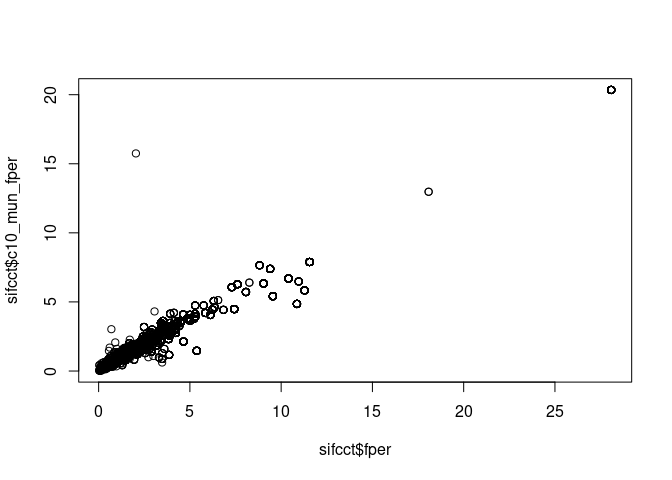
\includegraphics{analysis_1x_original_mail_v5_files/figure-latex/unnamed-chunk-3-1.pdf}

\begin{Shaded}
\begin{Highlighting}[]
\KeywordTok{cor}\NormalTok{(sifcct}\OperatorTok{$}\NormalTok{fper, sifcct}\OperatorTok{$}\NormalTok{c10_mun_fper, }\DataTypeTok{use=}\StringTok{"pairwise"}\NormalTok{)}
\end{Highlighting}
\end{Shaded}

\begin{verbatim}
## [1] 0.972352
\end{verbatim}

\begin{Shaded}
\begin{Highlighting}[]
\KeywordTok{plot}\NormalTok{(sifcct}\OperatorTok{$}\NormalTok{c10_mun_fper, sifcct}\OperatorTok{$}\NormalTok{c10_sreg_fper)}
\end{Highlighting}
\end{Shaded}

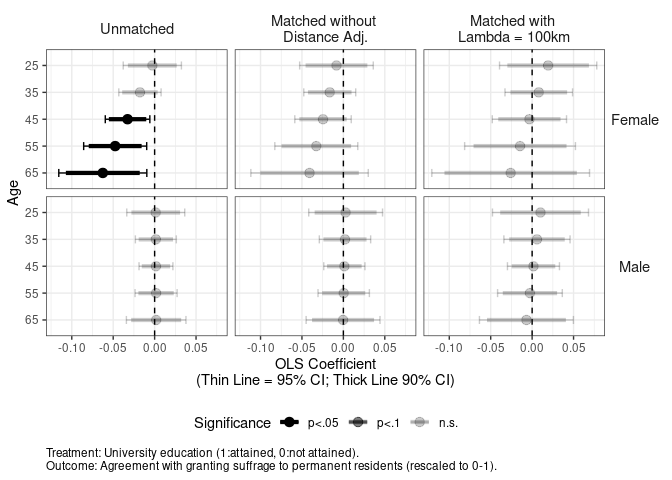
\includegraphics{analysis_1x_original_mail_v5_files/figure-latex/unnamed-chunk-3-2.pdf}

\begin{Shaded}
\begin{Highlighting}[]
\KeywordTok{cor}\NormalTok{(sifcct}\OperatorTok{$}\NormalTok{c10_mun_fper, sifcct}\OperatorTok{$}\NormalTok{c10_sreg_fper, }\DataTypeTok{use=}\StringTok{"pairwise"}\NormalTok{)}
\end{Highlighting}
\end{Shaded}

\begin{verbatim}
## [1] 0.6087222
\end{verbatim}

\begin{Shaded}
\begin{Highlighting}[]
\CommentTok{## MAIL ##}

\CommentTok{## Binary Age Cohort (50s or over)}
\NormalTok{mail}\OperatorTok{$}\NormalTok{age2 <-}\StringTok{ }\KeywordTok{ifelse}\NormalTok{(mail}\OperatorTok{$}\NormalTok{age }\OperatorTok{>=}\StringTok{ }\DecValTok{50}\NormalTok{, }\DecValTok{1}\NormalTok{, }\DecValTok{0}\NormalTok{)}
\NormalTok{mail}\OperatorTok{$}\NormalTok{agex <-}\StringTok{ }\NormalTok{mail}\OperatorTok{$}\NormalTok{age}\OperatorTok{/}\DecValTok{10} \OperatorTok{-}\StringTok{ }\FloatTok{4.5}
\CommentTok{## Small Region Foreiner Percent}
\NormalTok{mail}\OperatorTok{$}\NormalTok{c10_sreg_fper <-}\StringTok{ }\NormalTok{mail}\OperatorTok{$}\NormalTok{c10_sreg_foreignN}\OperatorTok{/}\NormalTok{mail}\OperatorTok{$}\NormalTok{c10_sreg_pop}\OperatorTok{*}\DecValTok{100}
\CommentTok{## Municipality Foreigner Percent}
\NormalTok{mail}\OperatorTok{$}\NormalTok{c10_mun_fper <-}\StringTok{ }\NormalTok{mail}\OperatorTok{$}\NormalTok{c10_mun_foreignN}\OperatorTok{/}\NormalTok{mail}\OperatorTok{$}\NormalTok{c10_mun_pop}\OperatorTok{*}\DecValTok{100}
\CommentTok{## Compare Census and Foreinger Registry Numbers}
\KeywordTok{plot}\NormalTok{(mail}\OperatorTok{$}\NormalTok{fper, mail}\OperatorTok{$}\NormalTok{c10_mun_fper)}
\end{Highlighting}
\end{Shaded}

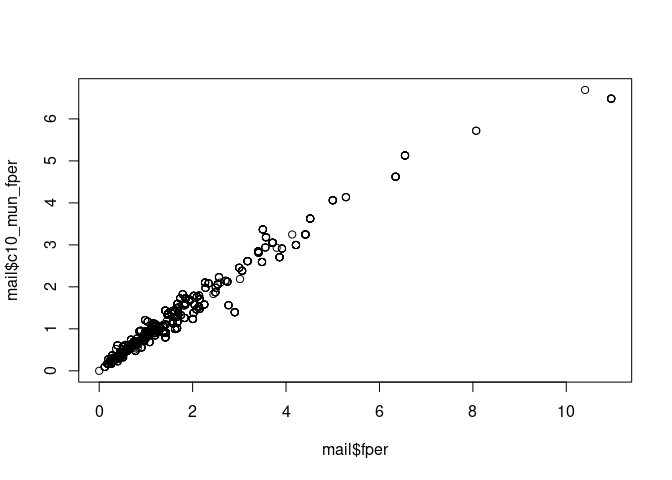
\includegraphics{analysis_1x_original_mail_v5_files/figure-latex/unnamed-chunk-3-3.pdf}

\begin{Shaded}
\begin{Highlighting}[]
\KeywordTok{cor}\NormalTok{(mail}\OperatorTok{$}\NormalTok{fper, mail}\OperatorTok{$}\NormalTok{c10_mun_fper, }\DataTypeTok{use=}\StringTok{"pairwise"}\NormalTok{)}
\end{Highlighting}
\end{Shaded}

\begin{verbatim}
## [1] 0.9782127
\end{verbatim}

\begin{Shaded}
\begin{Highlighting}[]
\KeywordTok{plot}\NormalTok{(mail}\OperatorTok{$}\NormalTok{c10_mun_fper, mail}\OperatorTok{$}\NormalTok{c10_sreg_fper)}
\end{Highlighting}
\end{Shaded}

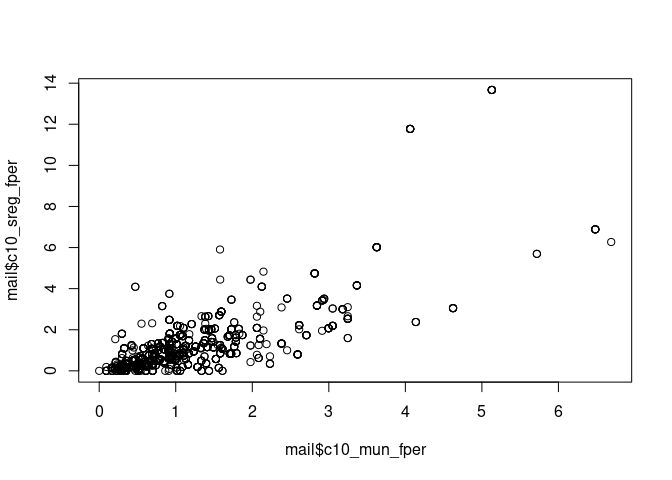
\includegraphics{analysis_1x_original_mail_v5_files/figure-latex/unnamed-chunk-3-4.pdf}

\begin{Shaded}
\begin{Highlighting}[]
\KeywordTok{cor}\NormalTok{(mail}\OperatorTok{$}\NormalTok{c10_mun_fper, mail}\OperatorTok{$}\NormalTok{c10_sreg_fper, }\DataTypeTok{use=}\StringTok{"pairwise"}\NormalTok{)}
\end{Highlighting}
\end{Shaded}

\begin{verbatim}
## [1] 0.7526452
\end{verbatim}

\begin{Shaded}
\begin{Highlighting}[]
\CommentTok{## Formula (SIFCCT) ##}

\NormalTok{basemod0 <-}\StringTok{ }\KeywordTok{formula}\NormalTok{(  }\OperatorTok{~}\StringTok{ }\NormalTok{edu2}\OperatorTok{*}\NormalTok{male}\OperatorTok{*}\NormalTok{agex }\OperatorTok{+}\StringTok{ }\NormalTok{lvpr }\OperatorTok{+}\StringTok{  }
\StringTok{                        }\KeywordTok{as.factor}\NormalTok{(wave)) }\CommentTok{# sifcct}
\NormalTok{basemodA <-}\StringTok{ }\KeywordTok{formula}\NormalTok{(  }\OperatorTok{~}\StringTok{ }\NormalTok{edu2}\OperatorTok{*}\NormalTok{male}\OperatorTok{*}\NormalTok{agex }\OperatorTok{+}\StringTok{ }\NormalTok{lvpr }\OperatorTok{+}\StringTok{  }
\StringTok{                        }\NormalTok{zip_did }\OperatorTok{+}\StringTok{ }\KeywordTok{sqrt}\NormalTok{(c10_sreg_fper) }\OperatorTok{+}\StringTok{ }\KeywordTok{I}\NormalTok{(c10_sreg_edu_ugsP}\OperatorTok{/}\DecValTok{10}\NormalTok{) }\OperatorTok{+}\StringTok{ }
\StringTok{                        }\KeywordTok{as.factor}\NormalTok{(wave)) }\CommentTok{# sifcct}
\NormalTok{basemodB <-}\StringTok{ }\KeywordTok{formula}\NormalTok{(  }\OperatorTok{~}\StringTok{ }\NormalTok{edu2}\OperatorTok{*}\NormalTok{male}\OperatorTok{*}\NormalTok{agex }\OperatorTok{+}\StringTok{ }\NormalTok{lvpr }\OperatorTok{+}\StringTok{  }
\StringTok{                        }\NormalTok{didper }\OperatorTok{+}\StringTok{ }\KeywordTok{sqrt}\NormalTok{(c10_mun_fper) }\OperatorTok{+}\StringTok{ }\KeywordTok{I}\NormalTok{(c10_mun_edu_ugsP}\OperatorTok{/}\DecValTok{10}\NormalTok{) }\OperatorTok{+}\StringTok{ }
\StringTok{                        }\KeywordTok{as.factor}\NormalTok{(wave)) }\CommentTok{# sifcct}
\NormalTok{basemodC <-}\StringTok{ }\KeywordTok{formula}\NormalTok{(  }\OperatorTok{~}\StringTok{ }\NormalTok{edu2}\OperatorTok{*}\NormalTok{male}\OperatorTok{*}\NormalTok{agex }\OperatorTok{+}\StringTok{ }\NormalTok{lvpr }\OperatorTok{+}\StringTok{  }
\StringTok{                        }\NormalTok{zip_did }\OperatorTok{+}\StringTok{ }\KeywordTok{sqrt}\NormalTok{(c10_sreg_fper) }\OperatorTok{+}\StringTok{ }\KeywordTok{I}\NormalTok{(c10_sreg_edu_ugsP}\OperatorTok{/}\DecValTok{10}\NormalTok{) }\OperatorTok{+}\StringTok{ }
\StringTok{                        }\NormalTok{didper }\OperatorTok{+}\StringTok{ }\KeywordTok{sqrt}\NormalTok{(c10_mun_fper) }\OperatorTok{+}\StringTok{ }\KeywordTok{I}\NormalTok{(c10_mun_edu_ugsP}\OperatorTok{/}\DecValTok{10}\NormalTok{) }\OperatorTok{+}\StringTok{ }
\StringTok{                        }\KeywordTok{as.factor}\NormalTok{(wave)) }\CommentTok{# sifcct}

\CommentTok{## Formula (SIFCCT.mlogit) ##}

\NormalTok{outmod0.mlogit <-}\StringTok{ }\KeywordTok{Formula}\NormalTok{(foreignsuff3x  }\OperatorTok{~}\StringTok{ }\DecValTok{0} \OperatorTok{|}\StringTok{ }\NormalTok{edu2}\OperatorTok{*}\NormalTok{male}\OperatorTok{*}\NormalTok{agex }\OperatorTok{+}\StringTok{ }\NormalTok{lvpr }\OperatorTok{+}\StringTok{  }
\StringTok{                            }\KeywordTok{as.factor}\NormalTok{(wave)) }\CommentTok{# sifcct}
\NormalTok{outmodA.mlogit <-}\StringTok{ }\KeywordTok{Formula}\NormalTok{(foreignsuff3x  }\OperatorTok{~}\StringTok{ }\DecValTok{0} \OperatorTok{|}\StringTok{ }\NormalTok{edu2}\OperatorTok{*}\NormalTok{male}\OperatorTok{*}\NormalTok{agex }\OperatorTok{+}\StringTok{ }\NormalTok{lvpr }\OperatorTok{+}\StringTok{  }
\StringTok{                            }\NormalTok{zip_did }\OperatorTok{+}\StringTok{ }\KeywordTok{sqrt}\NormalTok{(c10_sreg_fper) }\OperatorTok{+}\StringTok{ }\KeywordTok{I}\NormalTok{(c10_sreg_edu_ugsP}\OperatorTok{/}\DecValTok{10}\NormalTok{) }\OperatorTok{+}\StringTok{ }
\StringTok{                            }\KeywordTok{as.factor}\NormalTok{(wave)) }\CommentTok{# sifcct}
\NormalTok{outmodB.mlogit <-}\StringTok{ }\KeywordTok{Formula}\NormalTok{(foreignsuff3x  }\OperatorTok{~}\StringTok{ }\DecValTok{0} \OperatorTok{|}\StringTok{ }\NormalTok{edu2}\OperatorTok{*}\NormalTok{male}\OperatorTok{*}\NormalTok{agex }\OperatorTok{+}\StringTok{ }\NormalTok{lvpr }\OperatorTok{+}\StringTok{  }
\StringTok{                            }\NormalTok{didper }\OperatorTok{+}\StringTok{ }\KeywordTok{sqrt}\NormalTok{(c10_mun_fper) }\OperatorTok{+}\StringTok{ }\KeywordTok{I}\NormalTok{(c10_mun_edu_ugsP}\OperatorTok{/}\DecValTok{10}\NormalTok{) }\OperatorTok{+}\StringTok{ }
\StringTok{                            }\KeywordTok{as.factor}\NormalTok{(wave)) }\CommentTok{# sifcct}
\NormalTok{outmodC.mlogit <-}\StringTok{ }\KeywordTok{Formula}\NormalTok{(foreignsuff3x  }\OperatorTok{~}\StringTok{ }\DecValTok{0} \OperatorTok{|}\StringTok{ }\NormalTok{edu2}\OperatorTok{*}\NormalTok{male}\OperatorTok{*}\NormalTok{agex }\OperatorTok{+}\StringTok{ }\NormalTok{lvpr }\OperatorTok{+}\StringTok{  }
\StringTok{                            }\NormalTok{zip_did }\OperatorTok{+}\StringTok{ }\KeywordTok{sqrt}\NormalTok{(c10_sreg_fper) }\OperatorTok{+}\StringTok{ }\KeywordTok{I}\NormalTok{(c10_sreg_edu_ugsP}\OperatorTok{/}\DecValTok{10}\NormalTok{) }\OperatorTok{+}\StringTok{ }
\StringTok{                            }\NormalTok{didper }\OperatorTok{+}\StringTok{ }\KeywordTok{sqrt}\NormalTok{(c10_mun_fper) }\OperatorTok{+}\StringTok{ }\KeywordTok{I}\NormalTok{(c10_mun_edu_ugsP}\OperatorTok{/}\DecValTok{10}\NormalTok{) }\OperatorTok{+}\StringTok{ }
\StringTok{                            }\KeywordTok{as.factor}\NormalTok{(wave)) }\CommentTok{# sifcct}

\CommentTok{## Formula (MAIL) ##}

\NormalTok{basemod0m <-}\StringTok{ }\KeywordTok{formula}\NormalTok{(  }\OperatorTok{~}\StringTok{ }\NormalTok{edu2}\OperatorTok{*}\NormalTok{male}\OperatorTok{*}\NormalTok{agex }\OperatorTok{+}\StringTok{ }\NormalTok{lvpr) }\CommentTok{# sifcct}
\NormalTok{basemodAm <-}\StringTok{ }\KeywordTok{formula}\NormalTok{(  }\OperatorTok{~}\StringTok{ }\NormalTok{edu2}\OperatorTok{*}\NormalTok{male}\OperatorTok{*}\NormalTok{agex }\OperatorTok{+}\StringTok{ }\NormalTok{lvpr }\OperatorTok{+}\StringTok{  }
\StringTok{                         }\NormalTok{zip_did }\OperatorTok{+}\StringTok{ }\KeywordTok{sqrt}\NormalTok{(c10_sreg_fper) }\OperatorTok{+}\StringTok{ }\KeywordTok{I}\NormalTok{(c10_sreg_edu_ugsP}\OperatorTok{/}\DecValTok{10}\NormalTok{)) }\CommentTok{# sifcct}
\NormalTok{basemodBm <-}\StringTok{ }\KeywordTok{formula}\NormalTok{(  }\OperatorTok{~}\StringTok{ }\NormalTok{edu2}\OperatorTok{*}\NormalTok{male}\OperatorTok{*}\NormalTok{agex }\OperatorTok{+}\StringTok{ }\NormalTok{lvpr }\OperatorTok{+}\StringTok{  }
\StringTok{                         }\NormalTok{didper }\OperatorTok{+}\StringTok{ }\KeywordTok{sqrt}\NormalTok{(c10_mun_fper) }\OperatorTok{+}\StringTok{ }\KeywordTok{I}\NormalTok{(c10_mun_edu_ugsP}\OperatorTok{/}\DecValTok{10}\NormalTok{)) }\CommentTok{# sifcct}
\NormalTok{basemodCm <-}\StringTok{ }\KeywordTok{formula}\NormalTok{(  }\OperatorTok{~}\StringTok{ }\NormalTok{edu2}\OperatorTok{*}\NormalTok{male}\OperatorTok{*}\NormalTok{agex }\OperatorTok{+}\StringTok{ }\NormalTok{lvpr }\OperatorTok{+}\StringTok{  }
\StringTok{                         }\NormalTok{zip_did }\OperatorTok{+}\StringTok{ }\KeywordTok{sqrt}\NormalTok{(c10_sreg_fper) }\OperatorTok{+}\StringTok{ }\KeywordTok{I}\NormalTok{(c10_sreg_edu_ugsP}\OperatorTok{/}\DecValTok{10}\NormalTok{) }\OperatorTok{+}\StringTok{ }
\StringTok{                         }\NormalTok{didper }\OperatorTok{+}\StringTok{ }\KeywordTok{sqrt}\NormalTok{(c10_mun_fper) }\OperatorTok{+}\StringTok{ }\KeywordTok{I}\NormalTok{(c10_mun_edu_ugsP}\OperatorTok{/}\DecValTok{10}\NormalTok{)) }\CommentTok{# sifcct}

\CommentTok{## Formula (MAIL.mlogit) ##}

\NormalTok{outmod0m.mlogit <-}\StringTok{ }\KeywordTok{Formula}\NormalTok{(foreignsuff3x  }\OperatorTok{~}\StringTok{ }\DecValTok{0} \OperatorTok{|}\StringTok{ }\NormalTok{edu2}\OperatorTok{*}\NormalTok{male}\OperatorTok{*}\NormalTok{agex }\OperatorTok{+}\StringTok{ }\NormalTok{lvpr) }\CommentTok{# sifcct}
\NormalTok{outmodAm.mlogit <-}\StringTok{ }\KeywordTok{Formula}\NormalTok{(foreignsuff3x  }\OperatorTok{~}\StringTok{ }\DecValTok{0} \OperatorTok{|}\StringTok{ }\NormalTok{edu2}\OperatorTok{*}\NormalTok{male}\OperatorTok{*}\NormalTok{agex }\OperatorTok{+}\StringTok{ }\NormalTok{lvpr }\OperatorTok{+}\StringTok{  }
\StringTok{                             }\NormalTok{zip_did }\OperatorTok{+}\StringTok{ }\KeywordTok{sqrt}\NormalTok{(c10_sreg_fper) }\OperatorTok{+}\StringTok{ }\KeywordTok{I}\NormalTok{(c10_sreg_edu_ugsP}\OperatorTok{/}\DecValTok{10}\NormalTok{)) }\CommentTok{# sifcct}
\NormalTok{outmodBm.mlogit <-}\StringTok{ }\KeywordTok{Formula}\NormalTok{(foreignsuff3x  }\OperatorTok{~}\StringTok{ }\DecValTok{0} \OperatorTok{|}\StringTok{ }\NormalTok{edu2}\OperatorTok{*}\NormalTok{male}\OperatorTok{*}\NormalTok{agex }\OperatorTok{+}\StringTok{ }\NormalTok{lvpr }\OperatorTok{+}\StringTok{  }
\StringTok{                             }\NormalTok{didper }\OperatorTok{+}\StringTok{ }\KeywordTok{sqrt}\NormalTok{(c10_mun_fper) }\OperatorTok{+}\StringTok{ }\KeywordTok{I}\NormalTok{(c10_mun_edu_ugsP}\OperatorTok{/}\DecValTok{10}\NormalTok{)) }\CommentTok{# sifcct}
\NormalTok{outmodCm.mlogit <-}\StringTok{ }\KeywordTok{Formula}\NormalTok{(foreignsuff3x  }\OperatorTok{~}\StringTok{ }\DecValTok{0} \OperatorTok{|}\StringTok{ }\NormalTok{edu2}\OperatorTok{*}\NormalTok{male}\OperatorTok{*}\NormalTok{agex }\OperatorTok{+}\StringTok{ }\NormalTok{lvpr }\OperatorTok{+}\StringTok{  }
\StringTok{                             }\NormalTok{zip_did }\OperatorTok{+}\StringTok{ }\KeywordTok{sqrt}\NormalTok{(c10_sreg_fper) }\OperatorTok{+}\StringTok{ }\KeywordTok{I}\NormalTok{(c10_sreg_edu_ugsP}\OperatorTok{/}\DecValTok{10}\NormalTok{) }\OperatorTok{+}\StringTok{ }
\StringTok{                             }\NormalTok{didper }\OperatorTok{+}\StringTok{ }\KeywordTok{sqrt}\NormalTok{(c10_mun_fper) }\OperatorTok{+}\StringTok{ }\KeywordTok{I}\NormalTok{(c10_mun_edu_ugsP}\OperatorTok{/}\DecValTok{10}\NormalTok{)) }\CommentTok{# sifcct}

\CommentTok{## Variable Names ##}

\NormalTok{vnmap <-}\StringTok{ }\KeywordTok{list}\NormalTok{(}\StringTok{"edu2"}\NormalTok{ =}\StringTok{ "University education"}\NormalTok{,}
              \StringTok{"edu2 (1)"}\NormalTok{ =}\StringTok{ "University education"}\NormalTok{,}
              \StringTok{"female"}\NormalTok{ =}\StringTok{ "Gender (female)"}\NormalTok{,}
              \StringTok{"male"}\NormalTok{ =}\StringTok{ "Gender (male)"}\NormalTok{,}
              \StringTok{"male (1)"}\NormalTok{ =}\StringTok{ "Gender (male)"}\NormalTok{,}
              \StringTok{"age2"}\NormalTok{ =}\StringTok{ "Age 50s or older"}\NormalTok{,}
              \StringTok{"agex"}\NormalTok{ =}\StringTok{ "Age (by 10 years, centered at 45)"}\NormalTok{,}
              \StringTok{"edu2:female"}\NormalTok{ =}\StringTok{ "University * Female"}\NormalTok{,}
              \StringTok{"edu2:male"}\NormalTok{ =}\StringTok{ "University * Male"}\NormalTok{,}
              \StringTok{"edu2 (2)"}\NormalTok{ =}\StringTok{ "University * Male"}\NormalTok{,}
              \StringTok{"edu2:age2"}\NormalTok{ =}\StringTok{ "University * >=50s"}\NormalTok{,}
              \StringTok{"edu2:agex"}\NormalTok{ =}\StringTok{ "University * Age"}\NormalTok{,}
              \StringTok{"edu2 (3)"}\NormalTok{ =}\StringTok{ "University * Age"}\NormalTok{,}
              \StringTok{"edu2:female:age2"}\NormalTok{ =}\StringTok{ "University * Female * >=50s"}\NormalTok{,}
              \StringTok{"edu2:male:age2"}\NormalTok{ =}\StringTok{ "University * Male * >=50s"}\NormalTok{,}
              \StringTok{"edu2:female:agex"}\NormalTok{ =}\StringTok{ "University * Female * Age"}\NormalTok{,}
              \StringTok{"edu2:male:agex"}\NormalTok{ =}\StringTok{ "University * Male * Age"}\NormalTok{,}
              \StringTok{"edu2 (4)"}\NormalTok{ =}\StringTok{ "University * Male * Age"}\NormalTok{,}
              \StringTok{"female:age2"}\NormalTok{ =}\StringTok{ "Female * >=50s"}\NormalTok{,}
              \StringTok{"male:age2"}\NormalTok{ =}\StringTok{ "Male * >=50s"}\NormalTok{,}
              \StringTok{"female:agex"}\NormalTok{ =}\StringTok{ "Female * Age"}\NormalTok{,}
              \StringTok{"male:agex"}\NormalTok{ =}\StringTok{ "Male * Age"}\NormalTok{,}
              \StringTok{"male (2)"}\NormalTok{ =}\StringTok{ "Male * Age"}\NormalTok{,}
              \StringTok{"agecatMiddle Aged (40-50s)"}\NormalTok{ =}\StringTok{ "Middle Aged (40-50s)"}\NormalTok{,}
              \StringTok{"agecatElder (>=60s)"}\NormalTok{ =}\StringTok{ "Elder (>=60s)"}\NormalTok{,}
              \StringTok{"lvpr"}\NormalTok{ =}\StringTok{ "% of Life Residing Locally (zip)"}\NormalTok{,}
              \StringTok{"zip_did"}\NormalTok{ =}\StringTok{ "DID residence (zip)"}\NormalTok{,}
              \StringTok{"sqrt(c10_sreg_fper)"}\NormalTok{ =}\StringTok{ "Foreigner % sqrt. (zip)"}\NormalTok{,}
              \StringTok{"c10_sreg_edu_ugsP"}\NormalTok{ =}\StringTok{ "University % (zip)"}\NormalTok{,}
              \StringTok{"I(c10_sreg_edu_ugsP/10)"}\NormalTok{ =}\StringTok{ "University % by 10% (zip)"}\NormalTok{,}
              \StringTok{"didper"}\NormalTok{ =}\StringTok{ "DID proportion (mun.)"}\NormalTok{,}
              \StringTok{"sqrt(c10_mun_fper)"}\NormalTok{ =}\StringTok{ "Foreigner % sqrt. (mun.)"}\NormalTok{,}
              \StringTok{"I(c10_mun_edu_ugsP/10)"}\NormalTok{ =}\StringTok{ "University % by 10% (mun.)"}\NormalTok{,}
              \StringTok{"c10_mun_edu_ugsP"}\NormalTok{ =}\StringTok{ "University % (mun.)"}\NormalTok{)}
\end{Highlighting}
\end{Shaded}

\hypertarget{sifcct-outcome-model}{%
\section{SIFCCT: Outcome Model}\label{sifcct-outcome-model}}

\begin{Shaded}
\begin{Highlighting}[]
\CommentTok{## Living in Local ZIP since at least age 15 ##}

\NormalTok{smo_}\DecValTok{10}\NormalTok{ <-}\StringTok{ }\KeywordTok{lm}\NormalTok{(}\KeywordTok{update}\NormalTok{(foreignsuff }\OperatorTok{~}\StringTok{ }\NormalTok{., basemod0), }\DataTypeTok{data=}\NormalTok{sifcct[}\KeywordTok{which}\NormalTok{(sifcct}\OperatorTok{$}\NormalTok{age }\OperatorTok{-}\StringTok{ }\NormalTok{sifcct}\OperatorTok{$}\NormalTok{lvlen}\OperatorTok{>=}\DecValTok{23}\NormalTok{),])}
\NormalTok{smo_1A <-}\StringTok{ }\KeywordTok{lm}\NormalTok{(}\KeywordTok{update}\NormalTok{(foreignsuff }\OperatorTok{~}\StringTok{ }\NormalTok{., basemodA), }\DataTypeTok{data=}\NormalTok{sifcct[}\KeywordTok{which}\NormalTok{(sifcct}\OperatorTok{$}\NormalTok{age }\OperatorTok{-}\StringTok{ }\NormalTok{sifcct}\OperatorTok{$}\NormalTok{lvlen}\OperatorTok{>=}\DecValTok{23}\NormalTok{),])}
\NormalTok{smo_1B <-}\StringTok{ }\KeywordTok{lm}\NormalTok{(}\KeywordTok{update}\NormalTok{(foreignsuff }\OperatorTok{~}\StringTok{ }\NormalTok{., basemodB), }\DataTypeTok{data=}\NormalTok{sifcct[}\KeywordTok{which}\NormalTok{(sifcct}\OperatorTok{$}\NormalTok{age }\OperatorTok{-}\StringTok{ }\NormalTok{sifcct}\OperatorTok{$}\NormalTok{lvlen}\OperatorTok{>=}\DecValTok{23}\NormalTok{),])}
\NormalTok{smo_1C <-}\StringTok{ }\KeywordTok{lm}\NormalTok{(}\KeywordTok{update}\NormalTok{(foreignsuff }\OperatorTok{~}\StringTok{ }\NormalTok{., basemodC), }\DataTypeTok{data=}\NormalTok{sifcct[}\KeywordTok{which}\NormalTok{(sifcct}\OperatorTok{$}\NormalTok{age }\OperatorTok{-}\StringTok{ }\NormalTok{sifcct}\OperatorTok{$}\NormalTok{lvlen}\OperatorTok{>=}\DecValTok{23}\NormalTok{),])}

\KeywordTok{screenreg}\NormalTok{(}\KeywordTok{list}\NormalTok{(smo_}\DecValTok{10}\NormalTok{,smo_1A,smo_1B,smo_1C), }\DataTypeTok{digits =} \DecValTok{4}\NormalTok{, }\CommentTok{#single.row = T,}
          \DataTypeTok{override.se =} \KeywordTok{list}\NormalTok{(}\KeywordTok{coeftest}\NormalTok{(smo_}\DecValTok{10}\NormalTok{,}\DataTypeTok{vcov.=}\KeywordTok{vcovHC}\NormalTok{(smo_}\DecValTok{10}\NormalTok{))[,}\DecValTok{2}\NormalTok{],}
                             \KeywordTok{coeftest}\NormalTok{(smo_1A,}\DataTypeTok{vcov.=}\KeywordTok{vcovHC}\NormalTok{(smo_1A))[,}\DecValTok{2}\NormalTok{],}
                             \KeywordTok{coeftest}\NormalTok{(smo_1B,}\DataTypeTok{vcov.=}\KeywordTok{vcovHC}\NormalTok{(smo_1B))[,}\DecValTok{2}\NormalTok{],}
                             \KeywordTok{coeftest}\NormalTok{(smo_1C,}\DataTypeTok{vcov.=}\KeywordTok{vcovHC}\NormalTok{(smo_1C))[,}\DecValTok{2}\NormalTok{]),}
          \DataTypeTok{override.pvalues =} \KeywordTok{list}\NormalTok{(}\KeywordTok{coeftest}\NormalTok{(smo_}\DecValTok{10}\NormalTok{,}\DataTypeTok{vcov.=}\KeywordTok{vcovHC}\NormalTok{(smo_}\DecValTok{10}\NormalTok{))[,}\DecValTok{4}\NormalTok{],}
                                  \KeywordTok{coeftest}\NormalTok{(smo_1A,}\DataTypeTok{vcov.=}\KeywordTok{vcovHC}\NormalTok{(smo_1A))[,}\DecValTok{4}\NormalTok{],}
                                  \KeywordTok{coeftest}\NormalTok{(smo_1B,}\DataTypeTok{vcov.=}\KeywordTok{vcovHC}\NormalTok{(smo_1B))[,}\DecValTok{4}\NormalTok{],}
                                  \KeywordTok{coeftest}\NormalTok{(smo_1C,}\DataTypeTok{vcov.=}\KeywordTok{vcovHC}\NormalTok{(smo_1C))[,}\DecValTok{4}\NormalTok{]),}
          \DataTypeTok{omit.coef =} \StringTok{"(wave)"}\NormalTok{,}\DataTypeTok{stars =} \KeywordTok{c}\NormalTok{(}\FloatTok{0.1}\NormalTok{,}\FloatTok{0.05}\NormalTok{,}\FloatTok{0.01}\NormalTok{,}\FloatTok{0.001}\NormalTok{), }\DataTypeTok{symbol =} \StringTok{"+"}\NormalTok{,}
          \DataTypeTok{custom.coef.map =}\NormalTok{ vnmap, }
          \DataTypeTok{custom.model.names =} \KeywordTok{c}\NormalTok{(}\StringTok{"Base"}\NormalTok{,}\StringTok{"ZIP"}\NormalTok{,}\StringTok{"Municipality"}\NormalTok{,}\StringTok{"Full"}\NormalTok{))}
\end{Highlighting}
\end{Shaded}

\begin{verbatim}
## 
## =================================================================================================
##                                    Base            ZIP             Municipality    Full          
## -------------------------------------------------------------------------------------------------
## University education                  -0.0019         -0.0002         -0.0012         -0.0002    
##                                       (0.0063)        (0.0064)        (0.0063)        (0.0064)   
## Gender (male)                         -0.0560 ***     -0.0566 ***     -0.0564 ***     -0.0566 ***
##                                       (0.0076)        (0.0076)        (0.0076)        (0.0076)   
## Age (by 10 years, centered at 45)     -0.0126 ***     -0.0122 ***     -0.0124 ***     -0.0123 ***
##                                       (0.0034)        (0.0034)        (0.0034)        (0.0034)   
## University * Male                     -0.0208 *       -0.0204 *       -0.0206 *       -0.0205 *  
##                                       (0.0098)        (0.0098)        (0.0098)        (0.0098)   
## University * Age                       0.0125 *        0.0122 *        0.0123 *        0.0122 *  
##                                       (0.0051)        (0.0051)        (0.0051)        (0.0051)   
## University * Male * Age               -0.0045         -0.0041         -0.0043         -0.0041    
##                                       (0.0076)        (0.0076)        (0.0076)        (0.0076)   
## Male * Age                             0.0170 **       0.0166 **       0.0167 **       0.0166 ** 
##                                       (0.0057)        (0.0057)        (0.0057)        (0.0057)   
## % of Life Residing Locally (zip)      -0.0276 +       -0.0307 *       -0.0290 +       -0.0305 *  
##                                       (0.0149)        (0.0149)        (0.0149)        (0.0150)   
## DID residence (zip)                                   -0.0162 **                      -0.0190 ** 
##                                                       (0.0056)                        (0.0066)   
## Foreigner % sqrt. (zip)                               -0.0037                         -0.0021    
##                                                       (0.0039)                        (0.0054)   
## University % by 10% (zip)                             -0.0001                         -0.0024    
##                                                       (0.0025)                        (0.0036)   
## DID proportion (mun.)                                                 -0.0103          0.0077    
##                                                                       (0.0101)        (0.0119)   
## Foreigner % sqrt. (mun.)                                              -0.0071         -0.0049    
##                                                                       (0.0053)        (0.0074)   
## University % by 10% (mun.)                                             0.0012          0.0036    
##                                                                       (0.0038)        (0.0052)   
## -------------------------------------------------------------------------------------------------
## R^2                                    0.0122          0.0127          0.0124          0.0128    
## Adj. R^2                               0.0110          0.0115          0.0111          0.0114    
## Num. obs.                          24147           24147           24147           24147         
## =================================================================================================
## *** p < 0.001; ** p < 0.01; * p < 0.05; + p < 0.1
\end{verbatim}

\hypertarget{sifcct-outcome-model-2}{%
\section{SIFCCT: Outcome Model 2}\label{sifcct-outcome-model-2}}

\begin{Shaded}
\begin{Highlighting}[]
\CommentTok{## Living in Local ZIP since at least age 15 ##}

\CommentTok{# require(nnet)}
\CommentTok{# smo2_10 <- multinom(update(foreignsuff3x ~ ., basemod0), data=sifcct[which(sifcct$age - sifcct$lvlen>=23),])}
\CommentTok{# smo2_1A <- multinom(update(foreignsuff3x ~ ., basemodA), data=sifcct[which(sifcct$age - sifcct$lvlen>=23),])}
\CommentTok{# smo2_1B <- multinom(update(foreignsuff3x ~ ., basemodB), data=sifcct[which(sifcct$age - sifcct$lvlen>=23),])}
\CommentTok{# smo2_1C <- multinom(update(foreignsuff3x ~ ., basemodC), data=sifcct[which(sifcct$age - sifcct$lvlen>=23),])}

\NormalTok{sifcct.mlogit <-}\StringTok{ }\KeywordTok{dfidx}\NormalTok{(sifcct[}\KeywordTok{which}\NormalTok{(sifcct}\OperatorTok{$}\NormalTok{age }\OperatorTok{-}\StringTok{ }\NormalTok{sifcct}\OperatorTok{$}\NormalTok{lvlen}\OperatorTok{>=}\DecValTok{23}\NormalTok{),],}
                       \DataTypeTok{shape =} \StringTok{"wide"}\NormalTok{, }\DataTypeTok{choice =} \StringTok{"foreignsuff3x"}\NormalTok{)}
\CommentTok{# levels(sifcct.mlogit$idx$id2) <- c("Disagree","Neither","Agree")}
\NormalTok{smo2_}\DecValTok{10}\NormalTok{ <-}\StringTok{ }\KeywordTok{mlogit}\NormalTok{(outmod0.mlogit, }\DataTypeTok{data=}\NormalTok{sifcct.mlogit, }\DataTypeTok{reflevel=}\StringTok{"Disagree"}\NormalTok{)}
\NormalTok{smo2_1A <-}\StringTok{ }\KeywordTok{mlogit}\NormalTok{(outmodA.mlogit, }\DataTypeTok{data=}\NormalTok{sifcct.mlogit, }\DataTypeTok{reflevel=}\StringTok{"Disagree"}\NormalTok{)}
\NormalTok{smo2_1B <-}\StringTok{ }\KeywordTok{mlogit}\NormalTok{(outmodB.mlogit, }\DataTypeTok{data=}\NormalTok{sifcct.mlogit, }\DataTypeTok{reflevel=}\StringTok{"Disagree"}\NormalTok{)}
\NormalTok{smo2_1C <-}\StringTok{ }\KeywordTok{mlogit}\NormalTok{(outmodC.mlogit, }\DataTypeTok{data=}\NormalTok{sifcct.mlogit, }\DataTypeTok{reflevel=}\StringTok{"Disagree"}\NormalTok{)}

\KeywordTok{screenreg}\NormalTok{(}\KeywordTok{list}\NormalTok{(smo2_}\DecValTok{10}\NormalTok{,smo2_1A), }\DataTypeTok{digits =} \DecValTok{4}\NormalTok{, }\CommentTok{#single.row = T,}
          \DataTypeTok{override.se =} \KeywordTok{list}\NormalTok{(}\KeywordTok{coeftest}\NormalTok{(smo2_}\DecValTok{10}\NormalTok{,}\DataTypeTok{vcov=}\NormalTok{sandwich)[}\KeywordTok{grep}\NormalTok{(}\StringTok{":Neither"}\NormalTok{,}\KeywordTok{names}\NormalTok{(}\KeywordTok{coef}\NormalTok{(smo2_}\DecValTok{10}\NormalTok{))),}\DecValTok{2}\NormalTok{],}
                             \KeywordTok{coeftest}\NormalTok{(smo2_}\DecValTok{10}\NormalTok{,}\DataTypeTok{vcov=}\NormalTok{sandwich)[}\KeywordTok{grep}\NormalTok{(}\StringTok{":Agree"}\NormalTok{,}\KeywordTok{names}\NormalTok{(}\KeywordTok{coef}\NormalTok{(smo2_}\DecValTok{10}\NormalTok{))),}\DecValTok{2}\NormalTok{],}
                             \KeywordTok{coeftest}\NormalTok{(smo2_1A,}\DataTypeTok{vcov=}\NormalTok{sandwich)[}\KeywordTok{grep}\NormalTok{(}\StringTok{":Neither"}\NormalTok{,}\KeywordTok{names}\NormalTok{(}\KeywordTok{coef}\NormalTok{(smo2_1A))),}\DecValTok{2}\NormalTok{],}
                             \KeywordTok{coeftest}\NormalTok{(smo2_1A,}\DataTypeTok{vcov=}\NormalTok{sandwich)[}\KeywordTok{grep}\NormalTok{(}\StringTok{":Agree"}\NormalTok{,}\KeywordTok{names}\NormalTok{(}\KeywordTok{coef}\NormalTok{(smo2_1A))),}\DecValTok{2}\NormalTok{]),}
          \DataTypeTok{override.pvalues =} \KeywordTok{list}\NormalTok{(}\KeywordTok{coeftest}\NormalTok{(smo2_}\DecValTok{10}\NormalTok{,}\DataTypeTok{vcov=}\NormalTok{sandwich)[}\KeywordTok{grep}\NormalTok{(}\StringTok{":Neither"}\NormalTok{,}\KeywordTok{names}\NormalTok{(}\KeywordTok{coef}\NormalTok{(smo2_}\DecValTok{10}\NormalTok{))),}\DecValTok{4}\NormalTok{],}
                                  \KeywordTok{coeftest}\NormalTok{(smo2_}\DecValTok{10}\NormalTok{,}\DataTypeTok{vcov=}\NormalTok{sandwich)[}\KeywordTok{grep}\NormalTok{(}\StringTok{":Agree"}\NormalTok{,}\KeywordTok{names}\NormalTok{(}\KeywordTok{coef}\NormalTok{(smo2_}\DecValTok{10}\NormalTok{))),}\DecValTok{4}\NormalTok{],}
                                  \KeywordTok{coeftest}\NormalTok{(smo2_1A,}\DataTypeTok{vcov=}\NormalTok{sandwich)[}\KeywordTok{grep}\NormalTok{(}\StringTok{":Neither"}\NormalTok{,}\KeywordTok{names}\NormalTok{(}\KeywordTok{coef}\NormalTok{(smo2_1A))),}\DecValTok{4}\NormalTok{],}
                                  \KeywordTok{coeftest}\NormalTok{(smo2_1A,}\DataTypeTok{vcov=}\NormalTok{sandwich)[}\KeywordTok{grep}\NormalTok{(}\StringTok{":Agree"}\NormalTok{,}\KeywordTok{names}\NormalTok{(}\KeywordTok{coef}\NormalTok{(smo2_1A))),}\DecValTok{4}\NormalTok{]),}
          \DataTypeTok{beside =}\NormalTok{ T,}
          \DataTypeTok{omit.coef =} \StringTok{"(wave)"}\NormalTok{,}\DataTypeTok{stars =} \KeywordTok{c}\NormalTok{(}\FloatTok{0.1}\NormalTok{,}\FloatTok{0.05}\NormalTok{,}\FloatTok{0.01}\NormalTok{,}\FloatTok{0.001}\NormalTok{), }\DataTypeTok{symbol =} \StringTok{"+"}\NormalTok{, }
          \DataTypeTok{custom.model.names =} \KeywordTok{c}\NormalTok{(}\StringTok{"Base: Agree"}\NormalTok{,}\StringTok{"Base: Neither"}\NormalTok{,}
                                 \StringTok{"ZIP: Agree"}\NormalTok{,}\StringTok{"ZIP: Neither"}\NormalTok{),}
          \DataTypeTok{custom.coef.map =}\NormalTok{ vnmap)}
\end{Highlighting}
\end{Shaded}

\begin{verbatim}
## 
## =====================================================================================================
##                                    Base: Agree      Base: Neither    ZIP: Agree       ZIP: Neither   
## -----------------------------------------------------------------------------------------------------
## University education                    0.0063 ***      -0.3391           0.0199 ***      -0.3256    
##                                        (0.0498)         (0.0503)         (0.0503)         (0.0508)   
## Gender (male)                          -0.3609 ***      -0.5868 ***      -0.3662 ***      -0.5918 ***
##                                        (0.0563)         (0.0580)         (0.0563)         (0.0581)   
## Age (by 10 years, centered at 45)      -0.0835 ***      -0.1487 **       -0.0807 ***      -0.1470 ** 
##                                        (0.0271)         (0.0281)         (0.0272)         (0.0281)   
## University * Male                      -0.1262           0.0215 +        -0.1232           0.0239 +  
##                                        (0.0734)         (0.0738)         (0.0734)         (0.0738)   
## University * Age                        0.0947 *         0.1007 *         0.0927 *         0.0997 *  
##                                        (0.0398)         (0.0402)         (0.0398)         (0.0402)   
## University * Male * Age                -0.0331          -0.0377          -0.0301          -0.0370    
##                                        (0.0569)         (0.0563)         (0.0569)         (0.0564)   
## Male * Age                              0.1272           0.0550 **        0.1244           0.0535 ** 
##                                        (0.0428)         (0.0431)         (0.0428)         (0.0431)   
## % of Life Residing Locally (zip)       -0.2106          -0.0032 +        -0.2329          -0.0243 *  
##                                        (0.1123)         (0.1081)         (0.1128)         (0.1085)   
## DID residence (zip)                                                      -0.1274          -0.0373 ** 
##                                                                          (0.0418)         (0.0409)   
## Foreigner % sqrt. (zip)                                                  -0.0176          -0.0425    
##                                                                          (0.0290)         (0.0280)   
## University % by 10% (zip)                                                -0.0036          -0.0168    
##                                                                          (0.0185)         (0.0183)   
## -----------------------------------------------------------------------------------------------------
## AIC                                 51942.8378       51942.8378       51938.2602       51938.2602    
## Log Likelihood                     -25913.4189      -25913.4189      -25905.1301      -25905.1301    
## Num. obs.                           24147            24147            24147            24147         
## K                                       3                3                3                3         
## =====================================================================================================
## *** p < 0.001; ** p < 0.01; * p < 0.05; + p < 0.1
\end{verbatim}

\begin{Shaded}
\begin{Highlighting}[]
\KeywordTok{screenreg}\NormalTok{(}\KeywordTok{list}\NormalTok{(smo2_1B,smo2_1C), }\DataTypeTok{digits =} \DecValTok{4}\NormalTok{, }\CommentTok{#single.row = T,}
          \DataTypeTok{override.se =} \KeywordTok{list}\NormalTok{(}\KeywordTok{coeftest}\NormalTok{(smo2_1B,}\DataTypeTok{vcov=}\NormalTok{sandwich)[}\KeywordTok{grep}\NormalTok{(}\StringTok{":Neither"}\NormalTok{,}\KeywordTok{names}\NormalTok{(}\KeywordTok{coef}\NormalTok{(smo2_1B))),}\DecValTok{2}\NormalTok{],}
                             \KeywordTok{coeftest}\NormalTok{(smo2_1B,}\DataTypeTok{vcov=}\NormalTok{sandwich)[}\KeywordTok{grep}\NormalTok{(}\StringTok{":Agree"}\NormalTok{,}\KeywordTok{names}\NormalTok{(}\KeywordTok{coef}\NormalTok{(smo2_1B))),}\DecValTok{2}\NormalTok{],}
                             \KeywordTok{coeftest}\NormalTok{(smo2_1C,}\DataTypeTok{vcov=}\NormalTok{sandwich)[}\KeywordTok{grep}\NormalTok{(}\StringTok{":Neither"}\NormalTok{,}\KeywordTok{names}\NormalTok{(}\KeywordTok{coef}\NormalTok{(smo2_1C))),}\DecValTok{2}\NormalTok{],}
                             \KeywordTok{coeftest}\NormalTok{(smo2_1C,}\DataTypeTok{vcov=}\NormalTok{sandwich)[}\KeywordTok{grep}\NormalTok{(}\StringTok{":Agree"}\NormalTok{,}\KeywordTok{names}\NormalTok{(}\KeywordTok{coef}\NormalTok{(smo2_1C))),}\DecValTok{2}\NormalTok{]),}
          \DataTypeTok{override.pvalues =} \KeywordTok{list}\NormalTok{(}\KeywordTok{coeftest}\NormalTok{(smo2_1B,}\DataTypeTok{vcov=}\NormalTok{sandwich)[}\KeywordTok{grep}\NormalTok{(}\StringTok{":Neither"}\NormalTok{,}\KeywordTok{names}\NormalTok{(}\KeywordTok{coef}\NormalTok{(smo2_1B))),}\DecValTok{4}\NormalTok{],}
                                  \KeywordTok{coeftest}\NormalTok{(smo2_1B,}\DataTypeTok{vcov=}\NormalTok{sandwich)[}\KeywordTok{grep}\NormalTok{(}\StringTok{":Agree"}\NormalTok{,}\KeywordTok{names}\NormalTok{(}\KeywordTok{coef}\NormalTok{(smo2_1B))),}\DecValTok{4}\NormalTok{],}
                                  \KeywordTok{coeftest}\NormalTok{(smo2_1C,}\DataTypeTok{vcov=}\NormalTok{sandwich)[}\KeywordTok{grep}\NormalTok{(}\StringTok{":Neither"}\NormalTok{,}\KeywordTok{names}\NormalTok{(}\KeywordTok{coef}\NormalTok{(smo2_1C))),}\DecValTok{4}\NormalTok{],}
                                  \KeywordTok{coeftest}\NormalTok{(smo2_1C,}\DataTypeTok{vcov=}\NormalTok{sandwich)[}\KeywordTok{grep}\NormalTok{(}\StringTok{":Agree"}\NormalTok{,}\KeywordTok{names}\NormalTok{(}\KeywordTok{coef}\NormalTok{(smo2_1C))),}\DecValTok{4}\NormalTok{]),}
          \DataTypeTok{beside =}\NormalTok{ T,}
          \DataTypeTok{omit.coef =} \StringTok{"(wave)"}\NormalTok{,}\DataTypeTok{stars =} \KeywordTok{c}\NormalTok{(}\FloatTok{0.1}\NormalTok{,}\FloatTok{0.05}\NormalTok{,}\FloatTok{0.01}\NormalTok{,}\FloatTok{0.001}\NormalTok{), }\DataTypeTok{symbol =} \StringTok{"+"}\NormalTok{,}
          \DataTypeTok{custom.coef.map =}\NormalTok{ vnmap,}
          \DataTypeTok{custom.model.names =} \KeywordTok{c}\NormalTok{(}\StringTok{"Mun.: Agree"}\NormalTok{,}\StringTok{"Mun.: Neither"}\NormalTok{,}
                                 \StringTok{"Full: Agree"}\NormalTok{,}\StringTok{"Full: Neither"}\NormalTok{))}
\end{Highlighting}
\end{Shaded}

\begin{verbatim}
## 
## =====================================================================================================
##                                    Mun.: Agree      Mun.: Neither    Full: Agree      Full: Neither  
## -----------------------------------------------------------------------------------------------------
## University education                    0.0126 ***      -0.3328           0.0197 ***      -0.3261    
##                                        (0.0502)         (0.0506)         (0.0503)         (0.0508)   
## Gender (male)                          -0.3639 ***      -0.5893 ***      -0.3657 ***      -0.5914 ***
##                                        (0.0563)         (0.0581)         (0.0563)         (0.0581)   
## Age (by 10 years, centered at 45)      -0.0823 ***      -0.1478 **       -0.0813 ***      -0.1472 ** 
##                                        (0.0272)         (0.0281)         (0.0272)         (0.0281)   
## University * Male                      -0.1245           0.0226 +        -0.1238           0.0237 +  
##                                        (0.0734)         (0.0738)         (0.0734)         (0.0738)   
## University * Age                        0.0935 *         0.1001 *         0.0932 *         0.1004 *  
##                                        (0.0398)         (0.0402)         (0.0398)         (0.0402)   
## University * Male * Age                -0.0317          -0.0369          -0.0306          -0.0381    
##                                        (0.0569)         (0.0563)         (0.0569)         (0.0563)   
## Male * Age                              0.1256           0.0543 **        0.1248           0.0541 ** 
##                                        (0.0428)         (0.0431)         (0.0428)         (0.0431)   
## % of Life Residing Locally (zip)       -0.2215          -0.0098 *        -0.2318          -0.0260 *  
##                                        (0.1126)         (0.1083)         (0.1130)         (0.1087)   
## DID residence (zip)                                                      -0.1480          -0.0490 ** 
##                                                                          (0.0494)         (0.0483)   
## Foreigner % sqrt. (zip)                                                  -0.0169 +        -0.0685    
##                                                                          (0.0403)         (0.0391)   
## University % by 10% (zip)                                                -0.0157          -0.0262    
##                                                                          (0.0263)         (0.0261)   
## DID proportion (mun.)                  -0.0794          -0.0162           0.0607           0.0327    
##                                        (0.0752)         (0.0739)         (0.0887)         (0.0871)   
## Foreigner % sqrt. (mun.)               -0.0296          -0.0201          -0.0114           0.0436    
##                                        (0.0394)         (0.0388)         (0.0539)         (0.0536)   
## University % by 10% (mun.)              0.0003          -0.0162           0.0163           0.0113    
##                                        (0.0280)         (0.0275)         (0.0384)         (0.0380)   
## -----------------------------------------------------------------------------------------------------
## AIC                                 51951.2486       51951.2486       51948.0233       51948.0233    
## Log Likelihood                     -25911.6243      -25911.6243      -25904.0117      -25904.0117    
## Num. obs.                           24147            24147            24147            24147         
## K                                       3                3                3                3         
## =====================================================================================================
## *** p < 0.001; ** p < 0.01; * p < 0.05; + p < 0.1
\end{verbatim}

\hypertarget{sifcct-mediator-models}{%
\section{SIFCCT: Mediator Models}\label{sifcct-mediator-models}}

\hypertarget{knowledge}{%
\subsection{Knowledge}\label{knowledge}}

\begin{Shaded}
\begin{Highlighting}[]
\NormalTok{smm01_}\DecValTok{10}\NormalTok{ <-}\StringTok{ }\KeywordTok{lm}\NormalTok{(}\KeywordTok{update}\NormalTok{(knowledge }\OperatorTok{~}\StringTok{ }\NormalTok{., basemod0), }\DataTypeTok{data=}\NormalTok{sifcct[}\KeywordTok{which}\NormalTok{(sifcct}\OperatorTok{$}\NormalTok{age }\OperatorTok{-}\StringTok{ }\NormalTok{sifcct}\OperatorTok{$}\NormalTok{lvlen}\OperatorTok{>=}\DecValTok{23}\NormalTok{),])}
\NormalTok{smm01_1A <-}\StringTok{ }\KeywordTok{lm}\NormalTok{(}\KeywordTok{update}\NormalTok{(knowledge }\OperatorTok{~}\StringTok{ }\NormalTok{., basemodA), }\DataTypeTok{data=}\NormalTok{sifcct[}\KeywordTok{which}\NormalTok{(sifcct}\OperatorTok{$}\NormalTok{age }\OperatorTok{-}\StringTok{ }\NormalTok{sifcct}\OperatorTok{$}\NormalTok{lvlen}\OperatorTok{>=}\DecValTok{23}\NormalTok{),])}
\NormalTok{smm01_1B <-}\StringTok{ }\KeywordTok{lm}\NormalTok{(}\KeywordTok{update}\NormalTok{(knowledge }\OperatorTok{~}\StringTok{ }\NormalTok{., basemodB), }\DataTypeTok{data=}\NormalTok{sifcct[}\KeywordTok{which}\NormalTok{(sifcct}\OperatorTok{$}\NormalTok{age }\OperatorTok{-}\StringTok{ }\NormalTok{sifcct}\OperatorTok{$}\NormalTok{lvlen}\OperatorTok{>=}\DecValTok{23}\NormalTok{),])}
\NormalTok{smm01_1C <-}\StringTok{ }\KeywordTok{lm}\NormalTok{(}\KeywordTok{update}\NormalTok{(knowledge }\OperatorTok{~}\StringTok{ }\NormalTok{., basemodC), }\DataTypeTok{data=}\NormalTok{sifcct[}\KeywordTok{which}\NormalTok{(sifcct}\OperatorTok{$}\NormalTok{age }\OperatorTok{-}\StringTok{ }\NormalTok{sifcct}\OperatorTok{$}\NormalTok{lvlen}\OperatorTok{>=}\DecValTok{23}\NormalTok{),])}
\KeywordTok{screenreg}\NormalTok{(}\KeywordTok{list}\NormalTok{(smm01_}\DecValTok{10}\NormalTok{,smm01_1A,smm01_1B,smm01_1C), }\DataTypeTok{digits =} \DecValTok{4}\NormalTok{, }\CommentTok{#single.row = T,}
          \DataTypeTok{override.se =} \KeywordTok{list}\NormalTok{(}\KeywordTok{coeftest}\NormalTok{(smm01_}\DecValTok{10}\NormalTok{,}\DataTypeTok{vcov.=}\KeywordTok{vcovHC}\NormalTok{(smm01_}\DecValTok{10}\NormalTok{))[,}\DecValTok{2}\NormalTok{],}
                             \KeywordTok{coeftest}\NormalTok{(smm01_1A,}\DataTypeTok{vcov.=}\KeywordTok{vcovHC}\NormalTok{(smm01_1A))[,}\DecValTok{2}\NormalTok{],}
                             \KeywordTok{coeftest}\NormalTok{(smm01_1B,}\DataTypeTok{vcov.=}\KeywordTok{vcovHC}\NormalTok{(smm01_1B))[,}\DecValTok{2}\NormalTok{],}
                             \KeywordTok{coeftest}\NormalTok{(smm01_1C,}\DataTypeTok{vcov.=}\KeywordTok{vcovHC}\NormalTok{(smm01_1C))[,}\DecValTok{2}\NormalTok{]),}
          \DataTypeTok{override.pvalues =} \KeywordTok{list}\NormalTok{(}\KeywordTok{coeftest}\NormalTok{(smm01_}\DecValTok{10}\NormalTok{,}\DataTypeTok{vcov.=}\KeywordTok{vcovHC}\NormalTok{(smm01_}\DecValTok{10}\NormalTok{))[,}\DecValTok{4}\NormalTok{],}
                                  \KeywordTok{coeftest}\NormalTok{(smm01_1A,}\DataTypeTok{vcov.=}\KeywordTok{vcovHC}\NormalTok{(smm01_1A))[,}\DecValTok{4}\NormalTok{],}
                                  \KeywordTok{coeftest}\NormalTok{(smm01_1B,}\DataTypeTok{vcov.=}\KeywordTok{vcovHC}\NormalTok{(smm01_1B))[,}\DecValTok{4}\NormalTok{],}
                                  \KeywordTok{coeftest}\NormalTok{(smm01_1C,}\DataTypeTok{vcov.=}\KeywordTok{vcovHC}\NormalTok{(smm01_1C))[,}\DecValTok{4}\NormalTok{]),}
          \DataTypeTok{omit.coef =} \StringTok{"(wave)"}\NormalTok{, }\DataTypeTok{stars =} \KeywordTok{c}\NormalTok{(}\FloatTok{0.1}\NormalTok{,}\FloatTok{0.05}\NormalTok{,}\FloatTok{0.01}\NormalTok{,}\FloatTok{0.001}\NormalTok{), }\DataTypeTok{symbol =} \StringTok{"+"}\NormalTok{,}
          \DataTypeTok{custom.coef.map =}\NormalTok{ vnmap, }
          \DataTypeTok{custom.model.names =} \KeywordTok{c}\NormalTok{(}\StringTok{"Base"}\NormalTok{,}\StringTok{"ZIP"}\NormalTok{,}\StringTok{"Municipality"}\NormalTok{,}\StringTok{"Full"}\NormalTok{))}
\end{Highlighting}
\end{Shaded}

\begin{verbatim}
## 
## =================================================================================================
##                                    Base            ZIP             Municipality    Full          
## -------------------------------------------------------------------------------------------------
## University education                   0.1545 ***      0.1438 ***      0.1467 ***      0.1436 ***
##                                       (0.0058)        (0.0059)        (0.0059)        (0.0059)   
## Gender (male)                          0.1738 ***      0.1781 ***      0.1767 ***      0.1780 ***
##                                       (0.0069)        (0.0069)        (0.0069)        (0.0069)   
## Age (by 10 years, centered at 45)      0.0668 ***      0.0656 ***      0.0658 ***      0.0655 ***
##                                       (0.0032)        (0.0032)        (0.0032)        (0.0032)   
## University * Male                      0.0035          0.0017          0.0023          0.0018    
##                                       (0.0088)        (0.0087)        (0.0087)        (0.0087)   
## University * Age                      -0.0119 *       -0.0123 **      -0.0116 *       -0.0121 ** 
##                                       (0.0047)        (0.0047)        (0.0047)        (0.0047)   
## University * Male * Age               -0.0238 ***     -0.0238 ***     -0.0244 ***     -0.0240 ***
##                                       (0.0065)        (0.0065)        (0.0065)        (0.0065)   
## Male * Age                             0.0196 ***      0.0199 ***      0.0200 ***      0.0199 ***
##                                       (0.0050)        (0.0049)        (0.0049)        (0.0049)   
## % of Life Residing Locally (zip)      -0.0369 **      -0.0235 +       -0.0307 *       -0.0250 *  
##                                       (0.0127)        (0.0127)        (0.0127)        (0.0127)   
## DID residence (zip)                                    0.0079 +                        0.0108 +  
##                                                       (0.0047)                        (0.0056)   
## Foreigner % sqrt. (zip)                                0.0092 **                       0.0068    
##                                                       (0.0032)                        (0.0046)   
## University % by 10% (zip)                              0.0234 ***                      0.0179 ***
##                                                       (0.0021)                        (0.0030)   
## DID proportion (mun.)                                                 -0.0041         -0.0135    
##                                                                       (0.0086)        (0.0101)   
## Foreigner % sqrt. (mun.)                                               0.0086 +        0.0028    
##                                                                       (0.0044)        (0.0061)   
## University % by 10% (mun.)                                             0.0298 ***      0.0118 ** 
##                                                                       (0.0032)        (0.0044)   
## -------------------------------------------------------------------------------------------------
## R^2                                    0.2267          0.2325          0.2312          0.2328    
## Adj. R^2                               0.2258          0.2315          0.2302          0.2317    
## Num. obs.                          24147           24147           24147           24147         
## =================================================================================================
## *** p < 0.001; ** p < 0.01; * p < 0.05; + p < 0.1
\end{verbatim}

\hypertarget{ideology}{%
\subsection{Ideology}\label{ideology}}

\begin{Shaded}
\begin{Highlighting}[]
\NormalTok{smm02_}\DecValTok{10}\NormalTok{ <-}\StringTok{ }\KeywordTok{lm}\NormalTok{(}\KeywordTok{update}\NormalTok{(ideology }\OperatorTok{~}\StringTok{ }\NormalTok{., basemod0), }\DataTypeTok{data=}\NormalTok{sifcct[}\KeywordTok{which}\NormalTok{(sifcct}\OperatorTok{$}\NormalTok{age }\OperatorTok{-}\StringTok{ }\NormalTok{sifcct}\OperatorTok{$}\NormalTok{lvlen}\OperatorTok{>=}\DecValTok{23}\NormalTok{),])}
\NormalTok{smm02_1A <-}\StringTok{ }\KeywordTok{lm}\NormalTok{(}\KeywordTok{update}\NormalTok{(ideology }\OperatorTok{~}\StringTok{ }\NormalTok{., basemodA), }\DataTypeTok{data=}\NormalTok{sifcct[}\KeywordTok{which}\NormalTok{(sifcct}\OperatorTok{$}\NormalTok{age }\OperatorTok{-}\StringTok{ }\NormalTok{sifcct}\OperatorTok{$}\NormalTok{lvlen}\OperatorTok{>=}\DecValTok{23}\NormalTok{),])}
\NormalTok{smm02_1B <-}\StringTok{ }\KeywordTok{lm}\NormalTok{(}\KeywordTok{update}\NormalTok{(ideology }\OperatorTok{~}\StringTok{ }\NormalTok{., basemodB), }\DataTypeTok{data=}\NormalTok{sifcct[}\KeywordTok{which}\NormalTok{(sifcct}\OperatorTok{$}\NormalTok{age }\OperatorTok{-}\StringTok{ }\NormalTok{sifcct}\OperatorTok{$}\NormalTok{lvlen}\OperatorTok{>=}\DecValTok{23}\NormalTok{),])}
\NormalTok{smm02_1C <-}\StringTok{ }\KeywordTok{lm}\NormalTok{(}\KeywordTok{update}\NormalTok{(ideology }\OperatorTok{~}\StringTok{ }\NormalTok{., basemodC), }\DataTypeTok{data=}\NormalTok{sifcct[}\KeywordTok{which}\NormalTok{(sifcct}\OperatorTok{$}\NormalTok{age }\OperatorTok{-}\StringTok{ }\NormalTok{sifcct}\OperatorTok{$}\NormalTok{lvlen}\OperatorTok{>=}\DecValTok{23}\NormalTok{),])}
\KeywordTok{screenreg}\NormalTok{(}\KeywordTok{list}\NormalTok{(smm02_}\DecValTok{10}\NormalTok{,smm02_1A,smm02_1B,smm02_1C), }\DataTypeTok{digits =} \DecValTok{4}\NormalTok{, }\CommentTok{#single.row = T,}
          \DataTypeTok{override.se =} \KeywordTok{list}\NormalTok{(}\KeywordTok{coeftest}\NormalTok{(smm02_}\DecValTok{10}\NormalTok{,}\DataTypeTok{vcov.=}\KeywordTok{vcovHC}\NormalTok{(smm02_}\DecValTok{10}\NormalTok{))[,}\DecValTok{2}\NormalTok{],}
                             \KeywordTok{coeftest}\NormalTok{(smm02_1A,}\DataTypeTok{vcov.=}\KeywordTok{vcovHC}\NormalTok{(smm02_1A))[,}\DecValTok{2}\NormalTok{],}
                             \KeywordTok{coeftest}\NormalTok{(smm02_1B,}\DataTypeTok{vcov.=}\KeywordTok{vcovHC}\NormalTok{(smm02_1B))[,}\DecValTok{2}\NormalTok{],}
                             \KeywordTok{coeftest}\NormalTok{(smm02_1C,}\DataTypeTok{vcov.=}\KeywordTok{vcovHC}\NormalTok{(smm02_1C))[,}\DecValTok{2}\NormalTok{]),}
          \DataTypeTok{override.pvalues =} \KeywordTok{list}\NormalTok{(}\KeywordTok{coeftest}\NormalTok{(smm02_}\DecValTok{10}\NormalTok{,}\DataTypeTok{vcov.=}\KeywordTok{vcovHC}\NormalTok{(smm02_}\DecValTok{10}\NormalTok{))[,}\DecValTok{4}\NormalTok{],}
                                  \KeywordTok{coeftest}\NormalTok{(smm02_1A,}\DataTypeTok{vcov.=}\KeywordTok{vcovHC}\NormalTok{(smm02_1A))[,}\DecValTok{4}\NormalTok{],}
                                  \KeywordTok{coeftest}\NormalTok{(smm02_1B,}\DataTypeTok{vcov.=}\KeywordTok{vcovHC}\NormalTok{(smm02_1B))[,}\DecValTok{4}\NormalTok{],}
                                  \KeywordTok{coeftest}\NormalTok{(smm02_1C,}\DataTypeTok{vcov.=}\KeywordTok{vcovHC}\NormalTok{(smm02_1C))[,}\DecValTok{4}\NormalTok{]),}
          \DataTypeTok{omit.coef =} \StringTok{"(wave)"}\NormalTok{, }\DataTypeTok{stars =} \KeywordTok{c}\NormalTok{(}\FloatTok{0.1}\NormalTok{,}\FloatTok{0.05}\NormalTok{,}\FloatTok{0.01}\NormalTok{,}\FloatTok{0.001}\NormalTok{), }\DataTypeTok{symbol =} \StringTok{"+"}\NormalTok{,}
          \DataTypeTok{custom.coef.map =}\NormalTok{ vnmap, }
          \DataTypeTok{custom.model.names =} \KeywordTok{c}\NormalTok{(}\StringTok{"Base"}\NormalTok{,}\StringTok{"ZIP"}\NormalTok{,}\StringTok{"Municipality"}\NormalTok{,}\StringTok{"Full"}\NormalTok{))}
\end{Highlighting}
\end{Shaded}

\begin{verbatim}
## 
## =================================================================================================
##                                    Base            ZIP             Municipality    Full          
## -------------------------------------------------------------------------------------------------
## University education                  -0.0132 ***     -0.0130 ***     -0.0125 **      -0.0129 ***
##                                       (0.0039)        (0.0039)        (0.0039)        (0.0039)   
## Gender (male)                         -0.0377 ***     -0.0378 ***     -0.0379 ***     -0.0379 ***
##                                       (0.0052)        (0.0052)        (0.0052)        (0.0052)   
## Age (by 10 years, centered at 45)     -0.0082 ***     -0.0083 ***     -0.0081 ***     -0.0082 ***
##                                       (0.0022)        (0.0022)        (0.0022)        (0.0022)   
## University * Male                      0.0229 ***      0.0229 ***      0.0230 ***      0.0230 ***
##                                       (0.0065)        (0.0065)        (0.0065)        (0.0065)   
## University * Age                      -0.0061 +       -0.0059 +       -0.0061 +       -0.0060 +  
##                                       (0.0032)        (0.0032)        (0.0032)        (0.0032)   
## University * Male * Age               -0.0025         -0.0028         -0.0024         -0.0026    
##                                       (0.0050)        (0.0050)        (0.0050)        (0.0050)   
## Male * Age                             0.0144 ***      0.0146 ***      0.0144 ***      0.0145 ***
##                                       (0.0039)        (0.0039)        (0.0039)        (0.0039)   
## % of Life Residing Locally (zip)       0.0184 +        0.0184 +        0.0178 +        0.0182 +  
##                                       (0.0098)        (0.0098)        (0.0098)        (0.0098)   
## DID residence (zip)                                    0.0096 **                       0.0144 ***
##                                                       (0.0036)                        (0.0043)   
## Foreigner % sqrt. (zip)                               -0.0017                          0.0001    
##                                                       (0.0025)                        (0.0035)   
## University % by 10% (zip)                             -0.0023                         -0.0003    
##                                                       (0.0016)                        (0.0023)   
## DID proportion (mun.)                                                 -0.0009         -0.0146 +  
##                                                                       (0.0065)        (0.0077)   
## Foreigner % sqrt. (mun.)                                              -0.0012         -0.0016    
##                                                                       (0.0035)        (0.0047)   
## University % by 10% (mun.)                                            -0.0023         -0.0020    
##                                                                       (0.0024)        (0.0033)   
## -------------------------------------------------------------------------------------------------
## R^2                                    0.0069          0.0072          0.0069          0.0074    
## Adj. R^2                               0.0057          0.0059          0.0057          0.0060    
## Num. obs.                          24147           24147           24147           24147         
## =================================================================================================
## *** p < 0.001; ** p < 0.01; * p < 0.05; + p < 0.1
\end{verbatim}

\hypertarget{ldp---dpj-ft}{%
\subsection{LDP - DPJ FT}\label{ldp---dpj-ft}}

\begin{Shaded}
\begin{Highlighting}[]
\NormalTok{smm03_}\DecValTok{10}\NormalTok{ <-}\StringTok{ }\KeywordTok{lm}\NormalTok{(}\KeywordTok{update}\NormalTok{(ldpdpjft }\OperatorTok{~}\StringTok{ }\NormalTok{., basemod0), }\DataTypeTok{data=}\NormalTok{sifcct[}\KeywordTok{which}\NormalTok{(sifcct}\OperatorTok{$}\NormalTok{age }\OperatorTok{-}\StringTok{ }\NormalTok{sifcct}\OperatorTok{$}\NormalTok{lvlen}\OperatorTok{>=}\DecValTok{23}\NormalTok{),])}
\NormalTok{smm03_1A <-}\StringTok{ }\KeywordTok{lm}\NormalTok{(}\KeywordTok{update}\NormalTok{(ldpdpjft }\OperatorTok{~}\StringTok{ }\NormalTok{., basemodA), }\DataTypeTok{data=}\NormalTok{sifcct[}\KeywordTok{which}\NormalTok{(sifcct}\OperatorTok{$}\NormalTok{age }\OperatorTok{-}\StringTok{ }\NormalTok{sifcct}\OperatorTok{$}\NormalTok{lvlen}\OperatorTok{>=}\DecValTok{23}\NormalTok{),])}
\NormalTok{smm03_1B <-}\StringTok{ }\KeywordTok{lm}\NormalTok{(}\KeywordTok{update}\NormalTok{(ldpdpjft }\OperatorTok{~}\StringTok{ }\NormalTok{., basemodB), }\DataTypeTok{data=}\NormalTok{sifcct[}\KeywordTok{which}\NormalTok{(sifcct}\OperatorTok{$}\NormalTok{age }\OperatorTok{-}\StringTok{ }\NormalTok{sifcct}\OperatorTok{$}\NormalTok{lvlen}\OperatorTok{>=}\DecValTok{23}\NormalTok{),])}
\NormalTok{smm03_1C <-}\StringTok{ }\KeywordTok{lm}\NormalTok{(}\KeywordTok{update}\NormalTok{(ldpdpjft }\OperatorTok{~}\StringTok{ }\NormalTok{., basemodC), }\DataTypeTok{data=}\NormalTok{sifcct[}\KeywordTok{which}\NormalTok{(sifcct}\OperatorTok{$}\NormalTok{age }\OperatorTok{-}\StringTok{ }\NormalTok{sifcct}\OperatorTok{$}\NormalTok{lvlen}\OperatorTok{>=}\DecValTok{23}\NormalTok{),])}
\KeywordTok{screenreg}\NormalTok{(}\KeywordTok{list}\NormalTok{(smm03_}\DecValTok{10}\NormalTok{,smm03_1A,smm03_1B,smm03_1C), }\DataTypeTok{digits =} \DecValTok{4}\NormalTok{, }\CommentTok{#single.row = T,}
          \DataTypeTok{override.se =} \KeywordTok{list}\NormalTok{(}\KeywordTok{coeftest}\NormalTok{(smm03_}\DecValTok{10}\NormalTok{,}\DataTypeTok{vcov.=}\KeywordTok{vcovHC}\NormalTok{(smm03_}\DecValTok{10}\NormalTok{))[,}\DecValTok{2}\NormalTok{],}
                             \KeywordTok{coeftest}\NormalTok{(smm03_1A,}\DataTypeTok{vcov.=}\KeywordTok{vcovHC}\NormalTok{(smm03_1A))[,}\DecValTok{2}\NormalTok{],}
                             \KeywordTok{coeftest}\NormalTok{(smm03_1B,}\DataTypeTok{vcov.=}\KeywordTok{vcovHC}\NormalTok{(smm03_1B))[,}\DecValTok{2}\NormalTok{],}
                             \KeywordTok{coeftest}\NormalTok{(smm03_1C,}\DataTypeTok{vcov.=}\KeywordTok{vcovHC}\NormalTok{(smm03_1C))[,}\DecValTok{2}\NormalTok{]),}
          \DataTypeTok{override.pvalues =} \KeywordTok{list}\NormalTok{(}\KeywordTok{coeftest}\NormalTok{(smm03_}\DecValTok{10}\NormalTok{,}\DataTypeTok{vcov.=}\KeywordTok{vcovHC}\NormalTok{(smm03_}\DecValTok{10}\NormalTok{))[,}\DecValTok{4}\NormalTok{],}
                                  \KeywordTok{coeftest}\NormalTok{(smm03_1A,}\DataTypeTok{vcov.=}\KeywordTok{vcovHC}\NormalTok{(smm03_1A))[,}\DecValTok{4}\NormalTok{],}
                                  \KeywordTok{coeftest}\NormalTok{(smm03_1B,}\DataTypeTok{vcov.=}\KeywordTok{vcovHC}\NormalTok{(smm03_1B))[,}\DecValTok{4}\NormalTok{],}
                                  \KeywordTok{coeftest}\NormalTok{(smm03_1C,}\DataTypeTok{vcov.=}\KeywordTok{vcovHC}\NormalTok{(smm03_1C))[,}\DecValTok{4}\NormalTok{]),}
          \DataTypeTok{omit.coef =} \StringTok{"(wave)"}\NormalTok{, }\DataTypeTok{stars =} \KeywordTok{c}\NormalTok{(}\FloatTok{0.1}\NormalTok{,}\FloatTok{0.05}\NormalTok{,}\FloatTok{0.01}\NormalTok{,}\FloatTok{0.001}\NormalTok{), }\DataTypeTok{symbol =} \StringTok{"+"}\NormalTok{,}
          \DataTypeTok{custom.coef.map =}\NormalTok{ vnmap, }
          \DataTypeTok{custom.model.names =} \KeywordTok{c}\NormalTok{(}\StringTok{"Base"}\NormalTok{,}\StringTok{"ZIP"}\NormalTok{,}\StringTok{"Municipality"}\NormalTok{,}\StringTok{"Full"}\NormalTok{))}
\end{Highlighting}
\end{Shaded}

\begin{verbatim}
## 
## =================================================================================================
##                                    Base            ZIP             Municipality    Full          
## -------------------------------------------------------------------------------------------------
## University education                  -0.0122 ***     -0.0131 ***     -0.0125 ***     -0.0131 ***
##                                       (0.0030)        (0.0030)        (0.0030)        (0.0030)   
## Gender (male)                          0.0195 ***      0.0198 ***      0.0197 ***      0.0198 ***
##                                       (0.0037)        (0.0037)        (0.0037)        (0.0037)   
## Age (by 10 years, centered at 45)      0.0018          0.0016          0.0017          0.0016    
##                                       (0.0017)        (0.0017)        (0.0017)        (0.0017)   
## University * Male                      0.0093 +        0.0091 +        0.0092 +        0.0091 +  
##                                       (0.0047)        (0.0047)        (0.0047)        (0.0047)   
## University * Age                      -0.0097 ***     -0.0095 ***     -0.0096 ***     -0.0096 ***
##                                       (0.0025)        (0.0025)        (0.0025)        (0.0025)   
## University * Male * Age                0.0028          0.0027          0.0027          0.0027    
##                                       (0.0038)        (0.0038)        (0.0038)        (0.0038)   
## Male * Age                            -0.0072 *       -0.0070 *       -0.0070 *       -0.0070 *  
##                                       (0.0029)        (0.0029)        (0.0029)        (0.0029)   
## % of Life Residing Locally (zip)      -0.0062         -0.0046         -0.0056         -0.0043    
##                                       (0.0075)        (0.0075)        (0.0075)        (0.0075)   
## DID residence (zip)                                    0.0062 *                        0.0071 *  
##                                                       (0.0028)                        (0.0033)   
## Foreigner % sqrt. (zip)                                0.0038 *                        0.0049 +  
##                                                       (0.0019)                        (0.0027)   
## University % by 10% (zip)                              0.0001                          0.0018    
##                                                       (0.0012)                        (0.0018)   
## DID proportion (mun.)                                                  0.0050         -0.0019    
##                                                                       (0.0049)        (0.0058)   
## Foreigner % sqrt. (mun.)                                               0.0036         -0.0010    
##                                                                       (0.0026)        (0.0036)   
## University % by 10% (mun.)                                            -0.0011         -0.0031    
##                                                                       (0.0018)        (0.0025)   
## -------------------------------------------------------------------------------------------------
## R^2                                    0.1203          0.1207          0.1204          0.1208    
## Adj. R^2                               0.1192          0.1196          0.1193          0.1196    
## Num. obs.                          24147           24147           24147           24147         
## =================================================================================================
## *** p < 0.001; ** p < 0.01; * p < 0.05; + p < 0.1
\end{verbatim}

\hypertarget{favorability-of-south-korea}{%
\subsection{Favorability of South
Korea}\label{favorability-of-south-korea}}

\begin{Shaded}
\begin{Highlighting}[]
\NormalTok{smm04_}\DecValTok{10}\NormalTok{ <-}\StringTok{ }\KeywordTok{lm}\NormalTok{(}\KeywordTok{update}\NormalTok{(familiarityFT_KOR }\OperatorTok{~}\StringTok{ }\NormalTok{., basemod0), }\DataTypeTok{data=}\NormalTok{sifcct[}\KeywordTok{which}\NormalTok{(sifcct}\OperatorTok{$}\NormalTok{age }\OperatorTok{-}\StringTok{ }\NormalTok{sifcct}\OperatorTok{$}\NormalTok{lvlen}\OperatorTok{>=}\DecValTok{23}\NormalTok{),])}
\NormalTok{smm04_1A <-}\StringTok{ }\KeywordTok{lm}\NormalTok{(}\KeywordTok{update}\NormalTok{(familiarityFT_KOR }\OperatorTok{~}\StringTok{ }\NormalTok{., basemodA), }\DataTypeTok{data=}\NormalTok{sifcct[}\KeywordTok{which}\NormalTok{(sifcct}\OperatorTok{$}\NormalTok{age }\OperatorTok{-}\StringTok{ }\NormalTok{sifcct}\OperatorTok{$}\NormalTok{lvlen}\OperatorTok{>=}\DecValTok{23}\NormalTok{),])}
\NormalTok{smm04_1B <-}\StringTok{ }\KeywordTok{lm}\NormalTok{(}\KeywordTok{update}\NormalTok{(familiarityFT_KOR }\OperatorTok{~}\StringTok{ }\NormalTok{., basemodB), }\DataTypeTok{data=}\NormalTok{sifcct[}\KeywordTok{which}\NormalTok{(sifcct}\OperatorTok{$}\NormalTok{age }\OperatorTok{-}\StringTok{ }\NormalTok{sifcct}\OperatorTok{$}\NormalTok{lvlen}\OperatorTok{>=}\DecValTok{23}\NormalTok{),])}
\NormalTok{smm04_1C <-}\StringTok{ }\KeywordTok{lm}\NormalTok{(}\KeywordTok{update}\NormalTok{(familiarityFT_KOR }\OperatorTok{~}\StringTok{ }\NormalTok{., basemodC), }\DataTypeTok{data=}\NormalTok{sifcct[}\KeywordTok{which}\NormalTok{(sifcct}\OperatorTok{$}\NormalTok{age }\OperatorTok{-}\StringTok{ }\NormalTok{sifcct}\OperatorTok{$}\NormalTok{lvlen}\OperatorTok{>=}\DecValTok{23}\NormalTok{),])}
\KeywordTok{screenreg}\NormalTok{(}\KeywordTok{list}\NormalTok{(smm04_}\DecValTok{10}\NormalTok{,smm04_1A,smm04_1B,smm04_1C), }\DataTypeTok{digits =} \DecValTok{4}\NormalTok{, }\CommentTok{#single.row = T,}
          \DataTypeTok{override.se =} \KeywordTok{list}\NormalTok{(}\KeywordTok{coeftest}\NormalTok{(smm04_}\DecValTok{10}\NormalTok{,}\DataTypeTok{vcov.=}\KeywordTok{vcovHC}\NormalTok{(smm04_}\DecValTok{10}\NormalTok{))[,}\DecValTok{2}\NormalTok{],}
                             \KeywordTok{coeftest}\NormalTok{(smm04_1A,}\DataTypeTok{vcov.=}\KeywordTok{vcovHC}\NormalTok{(smm04_1A))[,}\DecValTok{2}\NormalTok{],}
                             \KeywordTok{coeftest}\NormalTok{(smm04_1B,}\DataTypeTok{vcov.=}\KeywordTok{vcovHC}\NormalTok{(smm04_1B))[,}\DecValTok{2}\NormalTok{],}
                             \KeywordTok{coeftest}\NormalTok{(smm04_1C,}\DataTypeTok{vcov.=}\KeywordTok{vcovHC}\NormalTok{(smm04_1C))[,}\DecValTok{2}\NormalTok{]),}
          \DataTypeTok{override.pvalues =} \KeywordTok{list}\NormalTok{(}\KeywordTok{coeftest}\NormalTok{(smm04_}\DecValTok{10}\NormalTok{,}\DataTypeTok{vcov.=}\KeywordTok{vcovHC}\NormalTok{(smm04_}\DecValTok{10}\NormalTok{))[,}\DecValTok{4}\NormalTok{],}
                                  \KeywordTok{coeftest}\NormalTok{(smm04_1A,}\DataTypeTok{vcov.=}\KeywordTok{vcovHC}\NormalTok{(smm04_1A))[,}\DecValTok{4}\NormalTok{],}
                                  \KeywordTok{coeftest}\NormalTok{(smm04_1B,}\DataTypeTok{vcov.=}\KeywordTok{vcovHC}\NormalTok{(smm04_1B))[,}\DecValTok{4}\NormalTok{],}
                                  \KeywordTok{coeftest}\NormalTok{(smm04_1C,}\DataTypeTok{vcov.=}\KeywordTok{vcovHC}\NormalTok{(smm04_1C))[,}\DecValTok{4}\NormalTok{]),}
          \DataTypeTok{omit.coef =} \StringTok{"(wave)"}\NormalTok{, }\DataTypeTok{stars =} \KeywordTok{c}\NormalTok{(}\FloatTok{0.1}\NormalTok{,}\FloatTok{0.05}\NormalTok{,}\FloatTok{0.01}\NormalTok{,}\FloatTok{0.001}\NormalTok{), }\DataTypeTok{symbol =} \StringTok{"+"}\NormalTok{,}
          \DataTypeTok{custom.coef.map =}\NormalTok{ vnmap, }
          \DataTypeTok{custom.model.names =} \KeywordTok{c}\NormalTok{(}\StringTok{"Base"}\NormalTok{,}\StringTok{"ZIP"}\NormalTok{,}\StringTok{"Municipality"}\NormalTok{,}\StringTok{"Full"}\NormalTok{))}
\end{Highlighting}
\end{Shaded}

\begin{verbatim}
## 
## =================================================================================================
##                                    Base            ZIP             Municipality    Full          
## -------------------------------------------------------------------------------------------------
## University education                   0.0100 *        0.0104 *        0.0099 +        0.0103 *  
##                                       (0.0050)        (0.0051)        (0.0050)        (0.0051)   
## Gender (male)                         -0.0589 ***     -0.0591 ***     -0.0590 ***     -0.0591 ***
##                                       (0.0057)        (0.0057)        (0.0057)        (0.0058)   
## Age (by 10 years, centered at 45)     -0.0015         -0.0014         -0.0015         -0.0014    
##                                       (0.0027)        (0.0027)        (0.0027)        (0.0027)   
## University * Male                      0.0077          0.0078          0.0078          0.0078    
##                                       (0.0074)        (0.0074)        (0.0074)        (0.0074)   
## University * Age                      -0.0001         -0.0002         -0.0001         -0.0001    
##                                       (0.0040)        (0.0040)        (0.0040)        (0.0040)   
## University * Male * Age                0.0004          0.0006          0.0005          0.0005    
##                                       (0.0057)        (0.0057)        (0.0057)        (0.0057)   
## Male * Age                             0.0272 ***      0.0271 ***      0.0272 ***      0.0271 ***
##                                       (0.0043)        (0.0043)        (0.0043)        (0.0043)   
## % of Life Residing Locally (zip)      -0.0209 +       -0.0218 *       -0.0215 *       -0.0222 *  
##                                       (0.0108)        (0.0109)        (0.0108)        (0.0109)   
## DID residence (zip)                                   -0.0083 *                       -0.0082 +  
##                                                       (0.0041)                        (0.0049)   
## Foreigner % sqrt. (zip)                                0.0004                         -0.0023    
##                                                       (0.0028)                        (0.0039)   
## University % by 10% (zip)                              0.0005                         -0.0009    
##                                                       (0.0018)                        (0.0026)   
## DID proportion (mun.)                                                 -0.0092         -0.0013    
##                                                                       (0.0073)        (0.0087)   
## Foreigner % sqrt. (mun.)                                               0.0025          0.0048    
##                                                                       (0.0039)        (0.0052)   
## University % by 10% (mun.)                                             0.0016          0.0026    
##                                                                       (0.0027)        (0.0038)   
## -------------------------------------------------------------------------------------------------
## R^2                                    0.0684          0.0686          0.0685          0.0686    
## Adj. R^2                               0.0673          0.0674          0.0673          0.0673    
## Num. obs.                          24147           24147           24147           24147         
## =================================================================================================
## *** p < 0.001; ** p < 0.01; * p < 0.05; + p < 0.1
\end{verbatim}

\hypertarget{favorability-of-china}{%
\subsection{Favorability of China}\label{favorability-of-china}}

\begin{Shaded}
\begin{Highlighting}[]
\NormalTok{smm05_}\DecValTok{10}\NormalTok{ <-}\StringTok{ }\KeywordTok{lm}\NormalTok{(}\KeywordTok{update}\NormalTok{(familiarityFT_CHN }\OperatorTok{~}\StringTok{ }\NormalTok{., basemod0), }\DataTypeTok{data=}\NormalTok{sifcct[}\KeywordTok{which}\NormalTok{(sifcct}\OperatorTok{$}\NormalTok{age }\OperatorTok{-}\StringTok{ }\NormalTok{sifcct}\OperatorTok{$}\NormalTok{lvlen}\OperatorTok{>=}\DecValTok{23}\NormalTok{),])}
\NormalTok{smm05_1A <-}\StringTok{ }\KeywordTok{lm}\NormalTok{(}\KeywordTok{update}\NormalTok{(familiarityFT_CHN }\OperatorTok{~}\StringTok{ }\NormalTok{., basemodA), }\DataTypeTok{data=}\NormalTok{sifcct[}\KeywordTok{which}\NormalTok{(sifcct}\OperatorTok{$}\NormalTok{age }\OperatorTok{-}\StringTok{ }\NormalTok{sifcct}\OperatorTok{$}\NormalTok{lvlen}\OperatorTok{>=}\DecValTok{23}\NormalTok{),])}
\NormalTok{smm05_1B <-}\StringTok{ }\KeywordTok{lm}\NormalTok{(}\KeywordTok{update}\NormalTok{(familiarityFT_CHN }\OperatorTok{~}\StringTok{ }\NormalTok{., basemodB), }\DataTypeTok{data=}\NormalTok{sifcct[}\KeywordTok{which}\NormalTok{(sifcct}\OperatorTok{$}\NormalTok{age }\OperatorTok{-}\StringTok{ }\NormalTok{sifcct}\OperatorTok{$}\NormalTok{lvlen}\OperatorTok{>=}\DecValTok{23}\NormalTok{),])}
\NormalTok{smm05_1C <-}\StringTok{ }\KeywordTok{lm}\NormalTok{(}\KeywordTok{update}\NormalTok{(familiarityFT_CHN }\OperatorTok{~}\StringTok{ }\NormalTok{., basemodC), }\DataTypeTok{data=}\NormalTok{sifcct[}\KeywordTok{which}\NormalTok{(sifcct}\OperatorTok{$}\NormalTok{age }\OperatorTok{-}\StringTok{ }\NormalTok{sifcct}\OperatorTok{$}\NormalTok{lvlen}\OperatorTok{>=}\DecValTok{23}\NormalTok{),])}
\KeywordTok{screenreg}\NormalTok{(}\KeywordTok{list}\NormalTok{(smm05_}\DecValTok{10}\NormalTok{,smm05_1A,smm05_1B,smm05_1C), }\DataTypeTok{digits =} \DecValTok{4}\NormalTok{, }\CommentTok{#single.row = T,}
          \DataTypeTok{override.se =} \KeywordTok{list}\NormalTok{(}\KeywordTok{coeftest}\NormalTok{(smm05_}\DecValTok{10}\NormalTok{,}\DataTypeTok{vcov.=}\KeywordTok{vcovHC}\NormalTok{(smm05_}\DecValTok{10}\NormalTok{))[,}\DecValTok{2}\NormalTok{],}
                             \KeywordTok{coeftest}\NormalTok{(smm05_1A,}\DataTypeTok{vcov.=}\KeywordTok{vcovHC}\NormalTok{(smm05_1A))[,}\DecValTok{2}\NormalTok{],}
                             \KeywordTok{coeftest}\NormalTok{(smm05_1B,}\DataTypeTok{vcov.=}\KeywordTok{vcovHC}\NormalTok{(smm05_1B))[,}\DecValTok{2}\NormalTok{],}
                             \KeywordTok{coeftest}\NormalTok{(smm05_1C,}\DataTypeTok{vcov.=}\KeywordTok{vcovHC}\NormalTok{(smm05_1C))[,}\DecValTok{2}\NormalTok{]),}
          \DataTypeTok{override.pvalues =} \KeywordTok{list}\NormalTok{(}\KeywordTok{coeftest}\NormalTok{(smm05_}\DecValTok{10}\NormalTok{,}\DataTypeTok{vcov.=}\KeywordTok{vcovHC}\NormalTok{(smm05_}\DecValTok{10}\NormalTok{))[,}\DecValTok{4}\NormalTok{],}
                                  \KeywordTok{coeftest}\NormalTok{(smm05_1A,}\DataTypeTok{vcov.=}\KeywordTok{vcovHC}\NormalTok{(smm05_1A))[,}\DecValTok{4}\NormalTok{],}
                                  \KeywordTok{coeftest}\NormalTok{(smm05_1B,}\DataTypeTok{vcov.=}\KeywordTok{vcovHC}\NormalTok{(smm05_1B))[,}\DecValTok{4}\NormalTok{],}
                                  \KeywordTok{coeftest}\NormalTok{(smm05_1C,}\DataTypeTok{vcov.=}\KeywordTok{vcovHC}\NormalTok{(smm05_1C))[,}\DecValTok{4}\NormalTok{]),}
          \DataTypeTok{omit.coef =} \StringTok{"(wave)"}\NormalTok{, }\DataTypeTok{stars =} \KeywordTok{c}\NormalTok{(}\FloatTok{0.1}\NormalTok{,}\FloatTok{0.05}\NormalTok{,}\FloatTok{0.01}\NormalTok{,}\FloatTok{0.001}\NormalTok{), }\DataTypeTok{symbol =} \StringTok{"+"}\NormalTok{,}
          \DataTypeTok{custom.coef.map =}\NormalTok{ vnmap, }
          \DataTypeTok{custom.model.names =} \KeywordTok{c}\NormalTok{(}\StringTok{"Base"}\NormalTok{,}\StringTok{"ZIP"}\NormalTok{,}\StringTok{"Municipality"}\NormalTok{,}\StringTok{"Full"}\NormalTok{))}
\end{Highlighting}
\end{Shaded}

\begin{verbatim}
## 
## =================================================================================================
##                                    Base            ZIP             Municipality    Full          
## -------------------------------------------------------------------------------------------------
## University education                   0.0201 ***      0.0196 ***      0.0190 ***      0.0194 ***
##                                       (0.0043)        (0.0043)        (0.0043)        (0.0043)   
## Gender (male)                         -0.0137 **      -0.0136 **      -0.0134 **      -0.0136 ** 
##                                       (0.0049)        (0.0050)        (0.0050)        (0.0050)   
## Age (by 10 years, centered at 45)     -0.0000         -0.0001         -0.0001         -0.0001    
##                                       (0.0024)        (0.0024)        (0.0024)        (0.0024)   
## University * Male                      0.0029          0.0029          0.0028          0.0029    
##                                       (0.0064)        (0.0064)        (0.0064)        (0.0064)   
## University * Age                      -0.0024         -0.0024         -0.0023         -0.0022    
##                                       (0.0034)        (0.0034)        (0.0034)        (0.0034)   
## University * Male * Age                0.0014          0.0015          0.0014          0.0013    
##                                       (0.0049)        (0.0049)        (0.0049)        (0.0049)   
## Male * Age                             0.0070 +        0.0070 +        0.0071 +        0.0071 +  
##                                       (0.0037)        (0.0037)        (0.0037)        (0.0037)   
## % of Life Residing Locally (zip)      -0.0257 **      -0.0250 **      -0.0252 **      -0.0259 ** 
##                                       (0.0094)        (0.0094)        (0.0094)        (0.0094)   
## DID residence (zip)                                   -0.0022                         -0.0014    
##                                                       (0.0035)                        (0.0041)   
## Foreigner % sqrt. (zip)                                0.0027                         -0.0008    
##                                                       (0.0024)                        (0.0033)   
## University % by 10% (zip)                              0.0009                         -0.0024    
##                                                       (0.0016)                        (0.0022)   
## DID proportion (mun.)                                                 -0.0064         -0.0052    
##                                                                       (0.0064)        (0.0075)   
## Foreigner % sqrt. (mun.)                                               0.0049          0.0055    
##                                                                       (0.0034)        (0.0046)   
## University % by 10% (mun.)                                             0.0042 +        0.0066 *  
##                                                                       (0.0024)        (0.0033)   
## -------------------------------------------------------------------------------------------------
## R^2                                    0.0241          0.0242          0.0244          0.0244    
## Adj. R^2                               0.0230          0.0229          0.0231          0.0231    
## Num. obs.                          24147           24147           24147           24147         
## =================================================================================================
## *** p < 0.001; ** p < 0.01; * p < 0.05; + p < 0.1
\end{verbatim}

\hypertarget{favorability-of-usa}{%
\subsection{Favorability of USA}\label{favorability-of-usa}}

\begin{Shaded}
\begin{Highlighting}[]
\NormalTok{smm06_}\DecValTok{10}\NormalTok{ <-}\StringTok{ }\KeywordTok{lm}\NormalTok{(}\KeywordTok{update}\NormalTok{(familiarityFT_USA }\OperatorTok{~}\StringTok{ }\NormalTok{., basemod0), }\DataTypeTok{data=}\NormalTok{sifcct[}\KeywordTok{which}\NormalTok{(sifcct}\OperatorTok{$}\NormalTok{age }\OperatorTok{-}\StringTok{ }\NormalTok{sifcct}\OperatorTok{$}\NormalTok{lvlen}\OperatorTok{>=}\DecValTok{23}\NormalTok{),])}
\NormalTok{smm06_1A <-}\StringTok{ }\KeywordTok{lm}\NormalTok{(}\KeywordTok{update}\NormalTok{(familiarityFT_USA }\OperatorTok{~}\StringTok{ }\NormalTok{., basemodA), }\DataTypeTok{data=}\NormalTok{sifcct[}\KeywordTok{which}\NormalTok{(sifcct}\OperatorTok{$}\NormalTok{age }\OperatorTok{-}\StringTok{ }\NormalTok{sifcct}\OperatorTok{$}\NormalTok{lvlen}\OperatorTok{>=}\DecValTok{23}\NormalTok{),])}
\NormalTok{smm06_1B <-}\StringTok{ }\KeywordTok{lm}\NormalTok{(}\KeywordTok{update}\NormalTok{(familiarityFT_USA }\OperatorTok{~}\StringTok{ }\NormalTok{., basemodB), }\DataTypeTok{data=}\NormalTok{sifcct[}\KeywordTok{which}\NormalTok{(sifcct}\OperatorTok{$}\NormalTok{age }\OperatorTok{-}\StringTok{ }\NormalTok{sifcct}\OperatorTok{$}\NormalTok{lvlen}\OperatorTok{>=}\DecValTok{23}\NormalTok{),])}
\NormalTok{smm06_1C <-}\StringTok{ }\KeywordTok{lm}\NormalTok{(}\KeywordTok{update}\NormalTok{(familiarityFT_USA }\OperatorTok{~}\StringTok{ }\NormalTok{., basemodC), }\DataTypeTok{data=}\NormalTok{sifcct[}\KeywordTok{which}\NormalTok{(sifcct}\OperatorTok{$}\NormalTok{age }\OperatorTok{-}\StringTok{ }\NormalTok{sifcct}\OperatorTok{$}\NormalTok{lvlen}\OperatorTok{>=}\DecValTok{23}\NormalTok{),])}
\KeywordTok{screenreg}\NormalTok{(}\KeywordTok{list}\NormalTok{(smm06_}\DecValTok{10}\NormalTok{,smm06_1A,smm06_1B,smm06_1C), }\DataTypeTok{digits =} \DecValTok{4}\NormalTok{, }\CommentTok{#single.row = T,}
          \DataTypeTok{override.se =} \KeywordTok{list}\NormalTok{(}\KeywordTok{coeftest}\NormalTok{(smm06_}\DecValTok{10}\NormalTok{,}\DataTypeTok{vcov.=}\KeywordTok{vcovHC}\NormalTok{(smm06_}\DecValTok{10}\NormalTok{))[,}\DecValTok{2}\NormalTok{],}
                             \KeywordTok{coeftest}\NormalTok{(smm06_1A,}\DataTypeTok{vcov.=}\KeywordTok{vcovHC}\NormalTok{(smm06_1A))[,}\DecValTok{2}\NormalTok{],}
                             \KeywordTok{coeftest}\NormalTok{(smm06_1B,}\DataTypeTok{vcov.=}\KeywordTok{vcovHC}\NormalTok{(smm06_1B))[,}\DecValTok{2}\NormalTok{],}
                             \KeywordTok{coeftest}\NormalTok{(smm06_1C,}\DataTypeTok{vcov.=}\KeywordTok{vcovHC}\NormalTok{(smm06_1C))[,}\DecValTok{2}\NormalTok{]),}
          \DataTypeTok{override.pvalues =} \KeywordTok{list}\NormalTok{(}\KeywordTok{coeftest}\NormalTok{(smm06_}\DecValTok{10}\NormalTok{,}\DataTypeTok{vcov.=}\KeywordTok{vcovHC}\NormalTok{(smm06_}\DecValTok{10}\NormalTok{))[,}\DecValTok{4}\NormalTok{],}
                                  \KeywordTok{coeftest}\NormalTok{(smm06_1A,}\DataTypeTok{vcov.=}\KeywordTok{vcovHC}\NormalTok{(smm06_1A))[,}\DecValTok{4}\NormalTok{],}
                                  \KeywordTok{coeftest}\NormalTok{(smm06_1B,}\DataTypeTok{vcov.=}\KeywordTok{vcovHC}\NormalTok{(smm06_1B))[,}\DecValTok{4}\NormalTok{],}
                                  \KeywordTok{coeftest}\NormalTok{(smm06_1C,}\DataTypeTok{vcov.=}\KeywordTok{vcovHC}\NormalTok{(smm06_1C))[,}\DecValTok{4}\NormalTok{]),}
          \DataTypeTok{omit.coef =} \StringTok{"(wave)"}\NormalTok{, }\DataTypeTok{stars =} \KeywordTok{c}\NormalTok{(}\FloatTok{0.1}\NormalTok{,}\FloatTok{0.05}\NormalTok{,}\FloatTok{0.01}\NormalTok{,}\FloatTok{0.001}\NormalTok{), }\DataTypeTok{symbol =} \StringTok{"+"}\NormalTok{,}
          \DataTypeTok{custom.coef.map =}\NormalTok{ vnmap, }
          \DataTypeTok{custom.model.names =} \KeywordTok{c}\NormalTok{(}\StringTok{"Base"}\NormalTok{,}\StringTok{"ZIP"}\NormalTok{,}\StringTok{"Municipality"}\NormalTok{,}\StringTok{"Full"}\NormalTok{))}
\end{Highlighting}
\end{Shaded}

\begin{verbatim}
## 
## =================================================================================================
##                                    Base            ZIP             Municipality    Full          
## -------------------------------------------------------------------------------------------------
## University education                   0.0128 **       0.0090 *        0.0104 *        0.0091 *  
##                                       (0.0041)        (0.0041)        (0.0041)        (0.0041)   
## Gender (male)                          0.0061          0.0077          0.0070          0.0077    
##                                       (0.0052)        (0.0052)        (0.0052)        (0.0052)   
## Age (by 10 years, centered at 45)      0.0080 ***      0.0076 ***      0.0077 ***      0.0076 ***
##                                       (0.0023)        (0.0023)        (0.0023)        (0.0023)   
## University * Male                      0.0215 ***      0.0209 **       0.0211 **       0.0209 ** 
##                                       (0.0065)        (0.0065)        (0.0065)        (0.0065)   
## University * Age                      -0.0045         -0.0048         -0.0044         -0.0048    
##                                       (0.0032)        (0.0032)        (0.0032)        (0.0032)   
## University * Male * Age               -0.0034         -0.0032         -0.0036         -0.0033    
##                                       (0.0049)        (0.0049)        (0.0049)        (0.0049)   
## Male * Age                             0.0207 ***      0.0206 ***      0.0208 ***      0.0207 ***
##                                       (0.0038)        (0.0038)        (0.0038)        (0.0038)   
## % of Life Residing Locally (zip)      -0.0151         -0.0107         -0.0130         -0.0104    
##                                       (0.0095)        (0.0095)        (0.0095)        (0.0095)   
## DID residence (zip)                                   -0.0036                         -0.0058    
##                                                       (0.0036)                        (0.0043)   
## Foreigner % sqrt. (zip)                                0.0030                          0.0025    
##                                                       (0.0025)                        (0.0034)   
## University % by 10% (zip)                              0.0096 ***                      0.0098 ***
##                                                       (0.0016)                        (0.0023)   
## DID proportion (mun.)                                                  0.0014          0.0075    
##                                                                       (0.0065)        (0.0076)   
## Foreigner % sqrt. (mun.)                                               0.0024          0.0006    
##                                                                       (0.0035)        (0.0047)   
## University % by 10% (mun.)                                             0.0086 ***     -0.0012    
##                                                                       (0.0024)        (0.0033)   
## -------------------------------------------------------------------------------------------------
## R^2                                    0.0324          0.0341          0.0334          0.0341    
## Adj. R^2                               0.0313          0.0328          0.0321          0.0328    
## Num. obs.                          24147           24147           24147           24147         
## =================================================================================================
## *** p < 0.001; ** p < 0.01; * p < 0.05; + p < 0.1
\end{verbatim}

\hypertarget{income}{%
\subsection{Income}\label{income}}

\begin{Shaded}
\begin{Highlighting}[]
\NormalTok{smm07_}\DecValTok{10}\NormalTok{ <-}\StringTok{ }\KeywordTok{lm}\NormalTok{(}\KeywordTok{update}\NormalTok{(income }\OperatorTok{~}\StringTok{ }\NormalTok{., basemod0), }\DataTypeTok{data=}\NormalTok{sifcct[}\KeywordTok{which}\NormalTok{(sifcct}\OperatorTok{$}\NormalTok{age }\OperatorTok{-}\StringTok{ }\NormalTok{sifcct}\OperatorTok{$}\NormalTok{lvlen}\OperatorTok{>=}\DecValTok{23}\NormalTok{),])}
\NormalTok{smm07_1A <-}\StringTok{ }\KeywordTok{lm}\NormalTok{(}\KeywordTok{update}\NormalTok{(income }\OperatorTok{~}\StringTok{ }\NormalTok{., basemodA), }\DataTypeTok{data=}\NormalTok{sifcct[}\KeywordTok{which}\NormalTok{(sifcct}\OperatorTok{$}\NormalTok{age }\OperatorTok{-}\StringTok{ }\NormalTok{sifcct}\OperatorTok{$}\NormalTok{lvlen}\OperatorTok{>=}\DecValTok{23}\NormalTok{),])}
\NormalTok{smm07_1B <-}\StringTok{ }\KeywordTok{lm}\NormalTok{(}\KeywordTok{update}\NormalTok{(income }\OperatorTok{~}\StringTok{ }\NormalTok{., basemodB), }\DataTypeTok{data=}\NormalTok{sifcct[}\KeywordTok{which}\NormalTok{(sifcct}\OperatorTok{$}\NormalTok{age }\OperatorTok{-}\StringTok{ }\NormalTok{sifcct}\OperatorTok{$}\NormalTok{lvlen}\OperatorTok{>=}\DecValTok{23}\NormalTok{),])}
\NormalTok{smm07_1C <-}\StringTok{ }\KeywordTok{lm}\NormalTok{(}\KeywordTok{update}\NormalTok{(income }\OperatorTok{~}\StringTok{ }\NormalTok{., basemodC), }\DataTypeTok{data=}\NormalTok{sifcct[}\KeywordTok{which}\NormalTok{(sifcct}\OperatorTok{$}\NormalTok{age }\OperatorTok{-}\StringTok{ }\NormalTok{sifcct}\OperatorTok{$}\NormalTok{lvlen}\OperatorTok{>=}\DecValTok{23}\NormalTok{),])}
\KeywordTok{screenreg}\NormalTok{(}\KeywordTok{list}\NormalTok{(smm07_}\DecValTok{10}\NormalTok{,smm07_1A,smm07_1B,smm07_1C), }\DataTypeTok{digits =} \DecValTok{4}\NormalTok{, }\CommentTok{#single.row = T,}
          \DataTypeTok{override.se =} \KeywordTok{list}\NormalTok{(}\KeywordTok{coeftest}\NormalTok{(smm07_}\DecValTok{10}\NormalTok{,}\DataTypeTok{vcov.=}\KeywordTok{vcovHC}\NormalTok{(smm07_}\DecValTok{10}\NormalTok{))[,}\DecValTok{2}\NormalTok{],}
                             \KeywordTok{coeftest}\NormalTok{(smm07_1A,}\DataTypeTok{vcov.=}\KeywordTok{vcovHC}\NormalTok{(smm07_1A))[,}\DecValTok{2}\NormalTok{],}
                             \KeywordTok{coeftest}\NormalTok{(smm07_1B,}\DataTypeTok{vcov.=}\KeywordTok{vcovHC}\NormalTok{(smm07_1B))[,}\DecValTok{2}\NormalTok{],}
                             \KeywordTok{coeftest}\NormalTok{(smm07_1C,}\DataTypeTok{vcov.=}\KeywordTok{vcovHC}\NormalTok{(smm07_1C))[,}\DecValTok{2}\NormalTok{]),}
          \DataTypeTok{override.pvalues =} \KeywordTok{list}\NormalTok{(}\KeywordTok{coeftest}\NormalTok{(smm07_}\DecValTok{10}\NormalTok{,}\DataTypeTok{vcov.=}\KeywordTok{vcovHC}\NormalTok{(smm07_}\DecValTok{10}\NormalTok{))[,}\DecValTok{4}\NormalTok{],}
                                  \KeywordTok{coeftest}\NormalTok{(smm07_1A,}\DataTypeTok{vcov.=}\KeywordTok{vcovHC}\NormalTok{(smm07_1A))[,}\DecValTok{4}\NormalTok{],}
                                  \KeywordTok{coeftest}\NormalTok{(smm07_1B,}\DataTypeTok{vcov.=}\KeywordTok{vcovHC}\NormalTok{(smm07_1B))[,}\DecValTok{4}\NormalTok{],}
                                  \KeywordTok{coeftest}\NormalTok{(smm07_1C,}\DataTypeTok{vcov.=}\KeywordTok{vcovHC}\NormalTok{(smm07_1C))[,}\DecValTok{4}\NormalTok{]),}
          \DataTypeTok{omit.coef =} \StringTok{"(wave)"}\NormalTok{, }\DataTypeTok{stars =} \KeywordTok{c}\NormalTok{(}\FloatTok{0.1}\NormalTok{,}\FloatTok{0.05}\NormalTok{,}\FloatTok{0.01}\NormalTok{,}\FloatTok{0.001}\NormalTok{), }\DataTypeTok{symbol =} \StringTok{"+"}\NormalTok{,}
          \DataTypeTok{custom.coef.map =}\NormalTok{ vnmap, }
          \DataTypeTok{custom.model.names =} \KeywordTok{c}\NormalTok{(}\StringTok{"Base"}\NormalTok{,}\StringTok{"ZIP"}\NormalTok{,}\StringTok{"Municipality"}\NormalTok{,}\StringTok{"Full"}\NormalTok{))}
\end{Highlighting}
\end{Shaded}

\begin{verbatim}
## 
## =================================================================================================
##                                    Base            ZIP             Municipality    Full          
## -------------------------------------------------------------------------------------------------
## University education                   0.0961 ***      0.0747 ***      0.0807 ***      0.0742 ***
##                                       (0.0054)        (0.0053)        (0.0053)        (0.0053)   
## Gender (male)                         -0.0430 ***     -0.0342 ***     -0.0374 ***     -0.0340 ***
##                                       (0.0059)        (0.0058)        (0.0058)        (0.0058)   
## Age (by 10 years, centered at 45)     -0.0049 +       -0.0072 *       -0.0069 *       -0.0072 *  
##                                       (0.0028)        (0.0028)        (0.0028)        (0.0028)   
## University * Male                      0.0385 ***      0.0350 ***      0.0362 ***      0.0351 ***
##                                       (0.0078)        (0.0076)        (0.0077)        (0.0076)   
## University * Age                       0.0332 ***      0.0320 ***      0.0342 ***      0.0325 ***
##                                       (0.0044)        (0.0043)        (0.0044)        (0.0043)   
## University * Male * Age               -0.0167 **      -0.0160 **      -0.0178 **      -0.0168 ** 
##                                       (0.0060)        (0.0060)        (0.0060)        (0.0060)   
## Male * Age                            -0.0056         -0.0055         -0.0045         -0.0051    
##                                       (0.0043)        (0.0043)        (0.0043)        (0.0043)   
## % of Life Residing Locally (zip)       0.1046 ***      0.1305 ***      0.1169 ***      0.1279 ***
##                                       (0.0127)        (0.0125)        (0.0126)        (0.0125)   
## DID residence (zip)                                   -0.0031                         -0.0028    
##                                                       (0.0044)                        (0.0052)   
## Foreigner % sqrt. (zip)                                0.0169 ***                     -0.0042    
##                                                       (0.0031)                        (0.0042)   
## University % by 10% (zip)                              0.0514 ***                      0.0455 ***
##                                                       (0.0020)                        (0.0029)   
## DID proportion (mun.)                                                 -0.0118         -0.0055    
##                                                                       (0.0080)        (0.0094)   
## Foreigner % sqrt. (mun.)                                               0.0326 ***      0.0386 ***
##                                                                       (0.0043)        (0.0059)   
## University % by 10% (mun.)                                             0.0549 ***      0.0095 *  
##                                                                       (0.0031)        (0.0042)   
## -------------------------------------------------------------------------------------------------
## R^2                                    0.0537          0.0847          0.0765          0.0866    
## Adj. R^2                               0.0526          0.0835          0.0754          0.0853    
## Num. obs.                          24147           24147           24147           24147         
## =================================================================================================
## *** p < 0.001; ** p < 0.01; * p < 0.05; + p < 0.1
\end{verbatim}

\hypertarget{mail-outcome-model}{%
\section{MAIL: Outcome Model}\label{mail-outcome-model}}

\begin{Shaded}
\begin{Highlighting}[]
\CommentTok{## Living in Local ZIP since at least age 15 ##}

\NormalTok{mmo_}\DecValTok{10}\NormalTok{ <-}\StringTok{ }\KeywordTok{lm}\NormalTok{(}\KeywordTok{update}\NormalTok{(foreignsuff }\OperatorTok{~}\StringTok{ }\NormalTok{., basemod0m), }\DataTypeTok{data=}\NormalTok{mail[}\KeywordTok{which}\NormalTok{(mail}\OperatorTok{$}\NormalTok{age }\OperatorTok{-}\StringTok{ }\NormalTok{mail}\OperatorTok{$}\NormalTok{lvlen}\OperatorTok{>=}\DecValTok{23}\NormalTok{),])}
\NormalTok{mmo_1A <-}\StringTok{ }\KeywordTok{lm}\NormalTok{(}\KeywordTok{update}\NormalTok{(foreignsuff }\OperatorTok{~}\StringTok{ }\NormalTok{., basemodAm), }\DataTypeTok{data=}\NormalTok{mail[}\KeywordTok{which}\NormalTok{(mail}\OperatorTok{$}\NormalTok{age }\OperatorTok{-}\StringTok{ }\NormalTok{mail}\OperatorTok{$}\NormalTok{lvlen}\OperatorTok{>=}\DecValTok{23}\NormalTok{),])}
\NormalTok{mmo_1B <-}\StringTok{ }\KeywordTok{lm}\NormalTok{(}\KeywordTok{update}\NormalTok{(foreignsuff }\OperatorTok{~}\StringTok{ }\NormalTok{., basemodBm), }\DataTypeTok{data=}\NormalTok{mail[}\KeywordTok{which}\NormalTok{(mail}\OperatorTok{$}\NormalTok{age }\OperatorTok{-}\StringTok{ }\NormalTok{mail}\OperatorTok{$}\NormalTok{lvlen}\OperatorTok{>=}\DecValTok{23}\NormalTok{),])}
\NormalTok{mmo_1C <-}\StringTok{ }\KeywordTok{lm}\NormalTok{(}\KeywordTok{update}\NormalTok{(foreignsuff }\OperatorTok{~}\StringTok{ }\NormalTok{., basemodCm), }\DataTypeTok{data=}\NormalTok{mail[}\KeywordTok{which}\NormalTok{(mail}\OperatorTok{$}\NormalTok{age }\OperatorTok{-}\StringTok{ }\NormalTok{mail}\OperatorTok{$}\NormalTok{lvlen}\OperatorTok{>=}\DecValTok{23}\NormalTok{),])}
\KeywordTok{screenreg}\NormalTok{(}\KeywordTok{list}\NormalTok{(mmo_}\DecValTok{10}\NormalTok{,mmo_1A,mmo_1B,mmo_1C), }\DataTypeTok{digits =} \DecValTok{4}\NormalTok{, }\CommentTok{#single.row = T,}
          \DataTypeTok{override.se =} \KeywordTok{list}\NormalTok{(}\KeywordTok{coeftest}\NormalTok{(mmo_}\DecValTok{10}\NormalTok{,}\DataTypeTok{vcov.=}\KeywordTok{vcovHC}\NormalTok{(mmo_}\DecValTok{10}\NormalTok{))[,}\DecValTok{2}\NormalTok{],}
                             \KeywordTok{coeftest}\NormalTok{(mmo_1A,}\DataTypeTok{vcov.=}\KeywordTok{vcovHC}\NormalTok{(mmo_1A))[,}\DecValTok{2}\NormalTok{],}
                             \KeywordTok{coeftest}\NormalTok{(mmo_1B,}\DataTypeTok{vcov.=}\KeywordTok{vcovHC}\NormalTok{(mmo_1B))[,}\DecValTok{2}\NormalTok{],}
                             \KeywordTok{coeftest}\NormalTok{(mmo_1C,}\DataTypeTok{vcov.=}\KeywordTok{vcovHC}\NormalTok{(mmo_1C))[,}\DecValTok{2}\NormalTok{]),}
          \DataTypeTok{override.pvalues =} \KeywordTok{list}\NormalTok{(}\KeywordTok{coeftest}\NormalTok{(mmo_}\DecValTok{10}\NormalTok{,}\DataTypeTok{vcov.=}\KeywordTok{vcovHC}\NormalTok{(mmo_}\DecValTok{10}\NormalTok{))[,}\DecValTok{4}\NormalTok{],}
                                  \KeywordTok{coeftest}\NormalTok{(mmo_1A,}\DataTypeTok{vcov.=}\KeywordTok{vcovHC}\NormalTok{(mmo_1A))[,}\DecValTok{4}\NormalTok{],}
                                  \KeywordTok{coeftest}\NormalTok{(mmo_1B,}\DataTypeTok{vcov.=}\KeywordTok{vcovHC}\NormalTok{(mmo_1B))[,}\DecValTok{4}\NormalTok{],}
                                  \KeywordTok{coeftest}\NormalTok{(mmo_1C,}\DataTypeTok{vcov.=}\KeywordTok{vcovHC}\NormalTok{(mmo_1C))[,}\DecValTok{4}\NormalTok{]),}
          \DataTypeTok{omit.coef =} \StringTok{"(wave)"}\NormalTok{,}\DataTypeTok{stars =} \KeywordTok{c}\NormalTok{(}\FloatTok{0.1}\NormalTok{,}\FloatTok{0.05}\NormalTok{,}\FloatTok{0.01}\NormalTok{,}\FloatTok{0.001}\NormalTok{), }\DataTypeTok{symbol =} \StringTok{"+"}\NormalTok{,}
          \DataTypeTok{custom.coef.map =}\NormalTok{ vnmap, }
          \DataTypeTok{custom.model.names =} \KeywordTok{c}\NormalTok{(}\StringTok{"Base"}\NormalTok{,}\StringTok{"ZIP"}\NormalTok{,}\StringTok{"Municipality"}\NormalTok{,}\StringTok{"Full"}\NormalTok{))}
\end{Highlighting}
\end{Shaded}

\begin{verbatim}
## 
## ====================================================================================
##                                    Base        ZIP          Municipality  Full      
## ------------------------------------------------------------------------------------
## University education                -0.0229     -0.0260      -0.0276       -0.0283  
##                                     (0.0514)    (0.0520)     (0.0524)      (0.0518) 
## Gender (male)                       -0.0666 +   -0.0596      -0.0625       -0.0564  
##                                     (0.0384)    (0.0389)     (0.0388)      (0.0391) 
## Age (by 10 years, centered at 45)   -0.0310 *   -0.0334 *    -0.0327 *     -0.0349 *
##                                     (0.0156)    (0.0156)     (0.0156)      (0.0156) 
## University * Male                   -0.0117     -0.0075      -0.0122       -0.0140  
##                                     (0.0688)    (0.0688)     (0.0690)      (0.0689) 
## University * Age                     0.0117      0.0134       0.0136        0.0156  
##                                     (0.0356)    (0.0354)     (0.0357)      (0.0355) 
## University * Male * Age              0.0057      0.0005      -0.0006       -0.0017  
##                                     (0.0452)    (0.0449)     (0.0452)      (0.0452) 
## Male * Age                          -0.0073     -0.0066      -0.0062       -0.0048  
##                                     (0.0211)    (0.0214)     (0.0213)      (0.0214) 
## % of Life Residing Locally (zip)     0.1703 +    0.1784 +     0.1816 *      0.1692 +
##                                     (0.0918)    (0.0923)     (0.0922)      (0.0926) 
## DID residence (zip)                              0.0415                     0.0758 +
##                                                 (0.0326)                   (0.0405) 
## Foreigner % sqrt. (zip)                         -0.0610 **                 -0.0666 *
##                                                 (0.0208)                   (0.0337) 
## University % by 10% (zip)                       -0.0009                    -0.0183  
##                                                 (0.0137)                   (0.0183) 
## DID proportion (mun.)                                        -0.0443       -0.1297 +
##                                                              (0.0577)      (0.0722) 
## Foreigner % sqrt. (mun.)                                     -0.0729 *      0.0018  
##                                                              (0.0329)      (0.0532) 
## University % by 10% (mun.)                                    0.0366        0.0571 +
##                                                              (0.0227)      (0.0303) 
## ------------------------------------------------------------------------------------
## R^2                                  0.0266      0.0371       0.0353        0.0438  
## Adj. R^2                             0.0158      0.0224       0.0206        0.0251  
## Num. obs.                          731         731          731           731       
## ====================================================================================
## *** p < 0.001; ** p < 0.01; * p < 0.05; + p < 0.1
\end{verbatim}

\hypertarget{mail-outcome-model-2}{%
\section{MAIL: Outcome Model 2}\label{mail-outcome-model-2}}

\begin{Shaded}
\begin{Highlighting}[]
\CommentTok{## Living in Local ZIP since at least age 15 ##}

\CommentTok{# require(nnet)}
\CommentTok{# mmo2_10 <- multinom(update(foreignsuff3x ~ ., basemod0), data=mail[which(mail$age - mail$lvlen>=23),])}
\CommentTok{# mmo2_1A <- multinom(update(foreignsuff3x ~ ., basemodA), data=mail[which(mail$age - mail$lvlen>=23),])}
\CommentTok{# mmo2_1B <- multinom(update(foreignsuff3x ~ ., basemodB), data=mail[which(mail$age - mail$lvlen>=23),])}
\CommentTok{# mmo2_1C <- multinom(update(foreignsuff3x ~ ., basemodC), data=mail[which(mail$age - mail$lvlen>=23),])}

\NormalTok{mail.mlogit <-}\StringTok{ }\KeywordTok{dfidx}\NormalTok{(mail[}\KeywordTok{which}\NormalTok{(mail}\OperatorTok{$}\NormalTok{age }\OperatorTok{-}\StringTok{ }\NormalTok{mail}\OperatorTok{$}\NormalTok{lvlen}\OperatorTok{>=}\DecValTok{23}\NormalTok{),],}
                     \DataTypeTok{shape =} \StringTok{"wide"}\NormalTok{, }\DataTypeTok{choice =} \StringTok{"foreignsuff3x"}\NormalTok{)}
\CommentTok{# levels(mail.mlogit$idx$id2) <- c("Disagree","Neither","Agree")}
\NormalTok{mmo2_}\DecValTok{10}\NormalTok{ <-}\StringTok{ }\KeywordTok{mlogit}\NormalTok{(outmod0m.mlogit, }\DataTypeTok{data=}\NormalTok{mail.mlogit, }\DataTypeTok{reflevel=}\StringTok{"Disagree"}\NormalTok{)}
\NormalTok{mmo2_1A <-}\StringTok{ }\KeywordTok{mlogit}\NormalTok{(outmodAm.mlogit, }\DataTypeTok{data=}\NormalTok{mail.mlogit, }\DataTypeTok{reflevel=}\StringTok{"Disagree"}\NormalTok{)}
\NormalTok{mmo2_1B <-}\StringTok{ }\KeywordTok{mlogit}\NormalTok{(outmodBm.mlogit, }\DataTypeTok{data=}\NormalTok{mail.mlogit, }\DataTypeTok{reflevel=}\StringTok{"Disagree"}\NormalTok{)}
\NormalTok{mmo2_1C <-}\StringTok{ }\KeywordTok{mlogit}\NormalTok{(outmodCm.mlogit, }\DataTypeTok{data=}\NormalTok{mail.mlogit, }\DataTypeTok{reflevel=}\StringTok{"Disagree"}\NormalTok{)}

\KeywordTok{screenreg}\NormalTok{(}\KeywordTok{list}\NormalTok{(mmo2_}\DecValTok{10}\NormalTok{,mmo2_1A), }\DataTypeTok{digits =} \DecValTok{4}\NormalTok{, }\CommentTok{#single.row = T,}
          \DataTypeTok{override.se =} \KeywordTok{list}\NormalTok{(}\KeywordTok{coeftest}\NormalTok{(mmo2_}\DecValTok{10}\NormalTok{,}\DataTypeTok{vcov=}\NormalTok{sandwich)[}\KeywordTok{grep}\NormalTok{(}\StringTok{":Neither"}\NormalTok{,}\KeywordTok{names}\NormalTok{(}\KeywordTok{coef}\NormalTok{(mmo2_}\DecValTok{10}\NormalTok{))),}\DecValTok{2}\NormalTok{],}
                             \KeywordTok{coeftest}\NormalTok{(mmo2_}\DecValTok{10}\NormalTok{,}\DataTypeTok{vcov=}\NormalTok{sandwich)[}\KeywordTok{grep}\NormalTok{(}\StringTok{":Agree"}\NormalTok{,}\KeywordTok{names}\NormalTok{(}\KeywordTok{coef}\NormalTok{(mmo2_}\DecValTok{10}\NormalTok{))),}\DecValTok{2}\NormalTok{],}
                             \KeywordTok{coeftest}\NormalTok{(mmo2_1A,}\DataTypeTok{vcov=}\NormalTok{sandwich)[}\KeywordTok{grep}\NormalTok{(}\StringTok{":Neither"}\NormalTok{,}\KeywordTok{names}\NormalTok{(}\KeywordTok{coef}\NormalTok{(mmo2_1A))),}\DecValTok{2}\NormalTok{],}
                             \KeywordTok{coeftest}\NormalTok{(mmo2_1A,}\DataTypeTok{vcov=}\NormalTok{sandwich)[}\KeywordTok{grep}\NormalTok{(}\StringTok{":Agree"}\NormalTok{,}\KeywordTok{names}\NormalTok{(}\KeywordTok{coef}\NormalTok{(mmo2_1A))),}\DecValTok{2}\NormalTok{]),}
          \DataTypeTok{override.pvalues =} \KeywordTok{list}\NormalTok{(}\KeywordTok{coeftest}\NormalTok{(mmo2_}\DecValTok{10}\NormalTok{,}\DataTypeTok{vcov=}\NormalTok{sandwich)[}\KeywordTok{grep}\NormalTok{(}\StringTok{":Neither"}\NormalTok{,}\KeywordTok{names}\NormalTok{(}\KeywordTok{coef}\NormalTok{(mmo2_}\DecValTok{10}\NormalTok{))),}\DecValTok{4}\NormalTok{],}
                                  \KeywordTok{coeftest}\NormalTok{(mmo2_}\DecValTok{10}\NormalTok{,}\DataTypeTok{vcov=}\NormalTok{sandwich)[}\KeywordTok{grep}\NormalTok{(}\StringTok{":Agree"}\NormalTok{,}\KeywordTok{names}\NormalTok{(}\KeywordTok{coef}\NormalTok{(mmo2_}\DecValTok{10}\NormalTok{))),}\DecValTok{4}\NormalTok{],}
                                  \KeywordTok{coeftest}\NormalTok{(mmo2_1A,}\DataTypeTok{vcov=}\NormalTok{sandwich)[}\KeywordTok{grep}\NormalTok{(}\StringTok{":Neither"}\NormalTok{,}\KeywordTok{names}\NormalTok{(}\KeywordTok{coef}\NormalTok{(mmo2_1A))),}\DecValTok{4}\NormalTok{],}
                                  \KeywordTok{coeftest}\NormalTok{(mmo2_1A,}\DataTypeTok{vcov=}\NormalTok{sandwich)[}\KeywordTok{grep}\NormalTok{(}\StringTok{":Agree"}\NormalTok{,}\KeywordTok{names}\NormalTok{(}\KeywordTok{coef}\NormalTok{(mmo2_1A))),}\DecValTok{4}\NormalTok{]),}
          \DataTypeTok{beside =}\NormalTok{ T,}
          \DataTypeTok{omit.coef =} \StringTok{"(wave)"}\NormalTok{,}\DataTypeTok{stars =} \KeywordTok{c}\NormalTok{(}\FloatTok{0.1}\NormalTok{,}\FloatTok{0.05}\NormalTok{,}\FloatTok{0.01}\NormalTok{,}\FloatTok{0.001}\NormalTok{), }\DataTypeTok{symbol =} \StringTok{"+"}\NormalTok{, }
          \DataTypeTok{custom.model.names =} \KeywordTok{c}\NormalTok{(}\StringTok{"Base: Agree"}\NormalTok{,}\StringTok{"Base: Neither"}\NormalTok{,}
                                 \StringTok{"ZIP: Agree"}\NormalTok{,}\StringTok{"ZIP: Neither"}\NormalTok{),}
          \DataTypeTok{custom.coef.map =}\NormalTok{ vnmap)}
\end{Highlighting}
\end{Shaded}

\begin{verbatim}
## 
## ==========================================================================================
##                                    Base: Agree   Base: Neither  ZIP: Agree    ZIP: Neither
## ------------------------------------------------------------------------------------------
## University education                 -0.1678 **    -1.1971        -0.2111 **    -1.3167   
##                                      (0.4300)      (0.3295)       (0.4353)      (0.3336)  
## Gender (male)                        -0.5387 *     -0.6271 +      -0.4887 +     -0.5641 + 
##                                      (0.3120)      (0.2846)       (0.3150)      (0.2897)  
## Age (by 10 years, centered at 45)    -0.2432 +     -0.2049 *      -0.2574 +     -0.2016 * 
##                                      (0.1186)      (0.1186)       (0.1200)      (0.1189)  
## University * Male                     0.0135        0.7116         0.0458        0.7193   
##                                      (0.5467)      (0.4391)       (0.5486)      (0.4420)  
## University * Age                      0.0381       -0.0742         0.0369       -0.1016   
##                                      (0.2899)      (0.2027)       (0.2889)      (0.2041)  
## University * Male * Age               0.1527        0.1059         0.1362        0.1666   
##                                      (0.3433)      (0.2646)       (0.3431)      (0.2663)  
## Male * Age                           -0.0460       -0.1025        -0.0490       -0.1335   
##                                      (0.1712)      (0.1532)       (0.1712)      (0.1565)  
## % of Life Residing Locally (zip)      1.1605 **     1.9066 +       1.2496 **     1.9965 * 
##                                      (0.6555)      (0.6021)       (0.6646)      (0.6079)  
## DID residence (zip)                                                0.2725        0.3398   
##                                                                   (0.2421)      (0.2182)  
## Foreigner % sqrt. (zip)                                           -0.3832        0.0860 * 
##                                                                   (0.1684)      (0.1535)  
## University % by 10% (zip)                                          0.0372        0.0763   
##                                                                   (0.1086)      (0.0954)  
## ------------------------------------------------------------------------------------------
## AIC                                1571.2886     1571.2886      1569.4923     1569.4923   
## Log Likelihood                     -767.6443     -767.6443      -760.7462     -760.7462   
## Num. obs.                           731           731            731           731        
## K                                     3             3              3             3        
## ==========================================================================================
## *** p < 0.001; ** p < 0.01; * p < 0.05; + p < 0.1
\end{verbatim}

\begin{Shaded}
\begin{Highlighting}[]
\KeywordTok{screenreg}\NormalTok{(}\KeywordTok{list}\NormalTok{(mmo2_1B,mmo2_1C), }\DataTypeTok{digits =} \DecValTok{4}\NormalTok{, }\CommentTok{#single.row = T,}
          \DataTypeTok{override.se =} \KeywordTok{list}\NormalTok{(}\KeywordTok{coeftest}\NormalTok{(mmo2_1B,}\DataTypeTok{vcov=}\NormalTok{sandwich)[}\KeywordTok{grep}\NormalTok{(}\StringTok{":Neither"}\NormalTok{,}\KeywordTok{names}\NormalTok{(}\KeywordTok{coef}\NormalTok{(mmo2_1B))),}\DecValTok{2}\NormalTok{],}
                             \KeywordTok{coeftest}\NormalTok{(mmo2_1B,}\DataTypeTok{vcov=}\NormalTok{sandwich)[}\KeywordTok{grep}\NormalTok{(}\StringTok{":Agree"}\NormalTok{,}\KeywordTok{names}\NormalTok{(}\KeywordTok{coef}\NormalTok{(mmo2_1B))),}\DecValTok{2}\NormalTok{],}
                             \KeywordTok{coeftest}\NormalTok{(mmo2_1C,}\DataTypeTok{vcov=}\NormalTok{sandwich)[}\KeywordTok{grep}\NormalTok{(}\StringTok{":Neither"}\NormalTok{,}\KeywordTok{names}\NormalTok{(}\KeywordTok{coef}\NormalTok{(mmo2_1C))),}\DecValTok{2}\NormalTok{],}
                             \KeywordTok{coeftest}\NormalTok{(mmo2_1C,}\DataTypeTok{vcov=}\NormalTok{sandwich)[}\KeywordTok{grep}\NormalTok{(}\StringTok{":Agree"}\NormalTok{,}\KeywordTok{names}\NormalTok{(}\KeywordTok{coef}\NormalTok{(mmo2_1C))),}\DecValTok{2}\NormalTok{]),}
          \DataTypeTok{override.pvalues =} \KeywordTok{list}\NormalTok{(}\KeywordTok{coeftest}\NormalTok{(mmo2_1B,}\DataTypeTok{vcov=}\NormalTok{sandwich)[}\KeywordTok{grep}\NormalTok{(}\StringTok{":Neither"}\NormalTok{,}\KeywordTok{names}\NormalTok{(}\KeywordTok{coef}\NormalTok{(mmo2_1B))),}\DecValTok{4}\NormalTok{],}
                                  \KeywordTok{coeftest}\NormalTok{(mmo2_1B,}\DataTypeTok{vcov=}\NormalTok{sandwich)[}\KeywordTok{grep}\NormalTok{(}\StringTok{":Agree"}\NormalTok{,}\KeywordTok{names}\NormalTok{(}\KeywordTok{coef}\NormalTok{(mmo2_1B))),}\DecValTok{4}\NormalTok{],}
                                  \KeywordTok{coeftest}\NormalTok{(mmo2_1C,}\DataTypeTok{vcov=}\NormalTok{sandwich)[}\KeywordTok{grep}\NormalTok{(}\StringTok{":Neither"}\NormalTok{,}\KeywordTok{names}\NormalTok{(}\KeywordTok{coef}\NormalTok{(mmo2_1C))),}\DecValTok{4}\NormalTok{],}
                                  \KeywordTok{coeftest}\NormalTok{(mmo2_1C,}\DataTypeTok{vcov=}\NormalTok{sandwich)[}\KeywordTok{grep}\NormalTok{(}\StringTok{":Agree"}\NormalTok{,}\KeywordTok{names}\NormalTok{(}\KeywordTok{coef}\NormalTok{(mmo2_1C))),}\DecValTok{4}\NormalTok{]),}
          \DataTypeTok{beside =}\NormalTok{ T,}
          \DataTypeTok{omit.coef =} \StringTok{"(wave)"}\NormalTok{,}\DataTypeTok{stars =} \KeywordTok{c}\NormalTok{(}\FloatTok{0.1}\NormalTok{,}\FloatTok{0.05}\NormalTok{,}\FloatTok{0.01}\NormalTok{,}\FloatTok{0.001}\NormalTok{), }\DataTypeTok{symbol =} \StringTok{"+"}\NormalTok{,}
          \DataTypeTok{custom.coef.map =}\NormalTok{ vnmap,}
          \DataTypeTok{custom.model.names =} \KeywordTok{c}\NormalTok{(}\StringTok{"Mun.: Agree"}\NormalTok{,}\StringTok{"Mun.: Neither"}\NormalTok{,}
                                 \StringTok{"Full: Agree"}\NormalTok{,}\StringTok{"Full: Neither"}\NormalTok{))}
\end{Highlighting}
\end{Shaded}

\begin{verbatim}
## 
## ===========================================================================================
##                                    Mun.: Agree   Mun.: Neither  Full: Agree   Full: Neither
## -------------------------------------------------------------------------------------------
## University education                 -0.2141 **    -1.2204        -0.2403 **    -1.3259    
##                                      (0.4344)      (0.3352)       (0.4362)      (0.3330)   
## Gender (male)                        -0.5128 +     -0.6133 +      -0.4807 +     -0.6069 +  
##                                      (0.3163)      (0.2894)       (0.3192)      (0.2916)   
## Age (by 10 years, centered at 45)    -0.2575 +     -0.2137 *      -0.2690       -0.1959 *  
##                                      (0.1203)      (0.1199)       (0.1212)      (0.1201)   
## University * Male                     0.0096        0.6956         0.0222        0.7643    
##                                      (0.5484)      (0.4437)       (0.5529)      (0.4442)   
## University * Age                      0.0514       -0.0708         0.0520       -0.0918    
##                                      (0.2936)      (0.2039)       (0.2911)      (0.2044)   
## University * Male * Age               0.1147        0.0835         0.1206        0.1381    
##                                      (0.3485)      (0.2661)       (0.3476)      (0.2676)   
## Male * Age                           -0.0383       -0.0920        -0.0388       -0.1338    
##                                      (0.1732)      (0.1552)       (0.1730)      (0.1573)   
## % of Life Residing Locally (zip)      1.2404 **     1.9352 *       1.2101 **     1.9534 *  
##                                      (0.6532)      (0.6039)       (0.6689)      (0.6096)   
## DID residence (zip)                                                0.4926 *      0.7561 +  
##                                                                   (0.2998)      (0.2741)   
## Foreigner % sqrt. (zip)                                           -0.3635 +      0.4838    
##                                                                   (0.2680)      (0.2385)   
## University % by 10% (zip)                                         -0.0505        0.1518    
##                                                                   (0.1407)      (0.1271)   
## DID proportion (mun.)                -0.2800       -0.5226        -0.7911 *     -1.1618    
##                                      (0.4207)      (0.3963)       (0.4999)      (0.5131)   
## Foreigner % sqrt. (mun.)             -0.4729       -0.1622 *      -0.1154 *     -0.8247    
##                                      (0.2602)      (0.2252)       (0.4150)      (0.3568)   
## University % by 10% (mun.)            0.2645        0.2493         0.3254        0.0623    
##                                      (0.1754)      (0.1615)       (0.2220)      (0.2103)   
## -------------------------------------------------------------------------------------------
## AIC                                1576.0771     1576.0771      1565.8437     1565.8437    
## Log Likelihood                     -764.0386     -764.0386      -752.9219     -752.9219    
## Num. obs.                           731           731            731           731         
## K                                     3             3              3             3         
## ===========================================================================================
## *** p < 0.001; ** p < 0.01; * p < 0.05; + p < 0.1
\end{verbatim}

\hypertarget{mail-mediator-models}{%
\section{MAIL: Mediator Models}\label{mail-mediator-models}}

\hypertarget{knowledge-1}{%
\subsection{Knowledge}\label{knowledge-1}}

\begin{Shaded}
\begin{Highlighting}[]
\NormalTok{mmm01_}\DecValTok{10}\NormalTok{ <-}\StringTok{ }\KeywordTok{lm}\NormalTok{(}\KeywordTok{update}\NormalTok{(knowledge }\OperatorTok{~}\StringTok{ }\NormalTok{., basemod0m), }\DataTypeTok{data=}\NormalTok{mail[}\KeywordTok{which}\NormalTok{(mail}\OperatorTok{$}\NormalTok{age }\OperatorTok{-}\StringTok{ }\NormalTok{mail}\OperatorTok{$}\NormalTok{lvlen}\OperatorTok{>=}\DecValTok{23}\NormalTok{),])}
\NormalTok{mmm01_1A <-}\StringTok{ }\KeywordTok{lm}\NormalTok{(}\KeywordTok{update}\NormalTok{(knowledge }\OperatorTok{~}\StringTok{ }\NormalTok{., basemodAm), }\DataTypeTok{data=}\NormalTok{mail[}\KeywordTok{which}\NormalTok{(mail}\OperatorTok{$}\NormalTok{age }\OperatorTok{-}\StringTok{ }\NormalTok{mail}\OperatorTok{$}\NormalTok{lvlen}\OperatorTok{>=}\DecValTok{23}\NormalTok{),])}
\NormalTok{mmm01_1B <-}\StringTok{ }\KeywordTok{lm}\NormalTok{(}\KeywordTok{update}\NormalTok{(knowledge }\OperatorTok{~}\StringTok{ }\NormalTok{., basemodBm), }\DataTypeTok{data=}\NormalTok{mail[}\KeywordTok{which}\NormalTok{(mail}\OperatorTok{$}\NormalTok{age }\OperatorTok{-}\StringTok{ }\NormalTok{mail}\OperatorTok{$}\NormalTok{lvlen}\OperatorTok{>=}\DecValTok{23}\NormalTok{),])}
\NormalTok{mmm01_1C <-}\StringTok{ }\KeywordTok{lm}\NormalTok{(}\KeywordTok{update}\NormalTok{(knowledge }\OperatorTok{~}\StringTok{ }\NormalTok{., basemodCm), }\DataTypeTok{data=}\NormalTok{mail[}\KeywordTok{which}\NormalTok{(mail}\OperatorTok{$}\NormalTok{age }\OperatorTok{-}\StringTok{ }\NormalTok{mail}\OperatorTok{$}\NormalTok{lvlen}\OperatorTok{>=}\DecValTok{23}\NormalTok{),])}
\KeywordTok{screenreg}\NormalTok{(}\KeywordTok{list}\NormalTok{(mmm01_}\DecValTok{10}\NormalTok{,mmm01_1A,mmm01_1B,mmm01_1C), }\DataTypeTok{digits =} \DecValTok{4}\NormalTok{, }\CommentTok{#single.row = T,}
          \DataTypeTok{override.se =} \KeywordTok{list}\NormalTok{(}\KeywordTok{coeftest}\NormalTok{(mmm01_}\DecValTok{10}\NormalTok{,}\DataTypeTok{vcov.=}\KeywordTok{vcovHC}\NormalTok{(mmm01_}\DecValTok{10}\NormalTok{))[,}\DecValTok{2}\NormalTok{],}
                             \KeywordTok{coeftest}\NormalTok{(mmm01_1A,}\DataTypeTok{vcov.=}\KeywordTok{vcovHC}\NormalTok{(mmm01_1A))[,}\DecValTok{2}\NormalTok{],}
                             \KeywordTok{coeftest}\NormalTok{(mmm01_1B,}\DataTypeTok{vcov.=}\KeywordTok{vcovHC}\NormalTok{(mmm01_1B))[,}\DecValTok{2}\NormalTok{],}
                             \KeywordTok{coeftest}\NormalTok{(mmm01_1C,}\DataTypeTok{vcov.=}\KeywordTok{vcovHC}\NormalTok{(mmm01_1C))[,}\DecValTok{2}\NormalTok{]),}
          \DataTypeTok{override.pvalues =} \KeywordTok{list}\NormalTok{(}\KeywordTok{coeftest}\NormalTok{(mmm01_}\DecValTok{10}\NormalTok{,}\DataTypeTok{vcov.=}\KeywordTok{vcovHC}\NormalTok{(mmm01_}\DecValTok{10}\NormalTok{))[,}\DecValTok{4}\NormalTok{],}
                                  \KeywordTok{coeftest}\NormalTok{(mmm01_1A,}\DataTypeTok{vcov.=}\KeywordTok{vcovHC}\NormalTok{(mmm01_1A))[,}\DecValTok{4}\NormalTok{],}
                                  \KeywordTok{coeftest}\NormalTok{(mmm01_1B,}\DataTypeTok{vcov.=}\KeywordTok{vcovHC}\NormalTok{(mmm01_1B))[,}\DecValTok{4}\NormalTok{],}
                                  \KeywordTok{coeftest}\NormalTok{(mmm01_1C,}\DataTypeTok{vcov.=}\KeywordTok{vcovHC}\NormalTok{(mmm01_1C))[,}\DecValTok{4}\NormalTok{]),}
          \DataTypeTok{omit.coef =} \StringTok{"(wave)"}\NormalTok{, }\DataTypeTok{stars =} \KeywordTok{c}\NormalTok{(}\FloatTok{0.1}\NormalTok{,}\FloatTok{0.05}\NormalTok{,}\FloatTok{0.01}\NormalTok{,}\FloatTok{0.001}\NormalTok{), }\DataTypeTok{symbol =} \StringTok{"+"}\NormalTok{,}
          \DataTypeTok{custom.coef.map =}\NormalTok{ vnmap, }
          \DataTypeTok{custom.model.names =} \KeywordTok{c}\NormalTok{(}\StringTok{"Base"}\NormalTok{,}\StringTok{"ZIP"}\NormalTok{,}\StringTok{"Municipality"}\NormalTok{,}\StringTok{"Full"}\NormalTok{))}
\end{Highlighting}
\end{Shaded}

\begin{verbatim}
## 
## =======================================================================================
##                                    Base          ZIP          Municipality  Full       
## ---------------------------------------------------------------------------------------
## University education                 0.1531 ***    0.1338 **    0.1347 **     0.1316 **
##                                     (0.0416)      (0.0415)     (0.0426)      (0.0421)  
## Gender (male)                        0.1057 **     0.1187 **    0.1156 **     0.1200 **
##                                     (0.0392)      (0.0393)     (0.0389)      (0.0392)  
## Age (by 10 years, centered at 45)    0.0073        0.0078       0.0064        0.0070   
##                                     (0.0150)      (0.0150)     (0.0151)      (0.0152)  
## University * Male                   -0.0010        0.0029      -0.0032        0.0009   
##                                     (0.0580)      (0.0577)     (0.0579)      (0.0577)  
## University * Age                     0.0314        0.0229       0.0288        0.0235   
##                                     (0.0331)      (0.0328)     (0.0336)      (0.0334)  
## University * Male * Age              0.0048        0.0127       0.0104        0.0129   
##                                     (0.0398)      (0.0397)     (0.0403)      (0.0401)  
## Male * Age                          -0.0032       -0.0068      -0.0056       -0.0062   
##                                     (0.0214)      (0.0216)     (0.0215)      (0.0216)  
## % of Life Residing Locally (zip)     0.0252        0.0525       0.0409        0.0525   
##                                     (0.0799)      (0.0806)     (0.0796)      (0.0811)  
## DID residence (zip)                                0.0216                     0.0060   
##                                                   (0.0286)                   (0.0348)  
## Foreigner % sqrt. (zip)                           -0.0108                    -0.0274   
##                                                   (0.0209)                   (0.0327)  
## University % by 10% (zip)                          0.0301 *                   0.0217   
##                                                   (0.0121)                   (0.0157)  
## DID proportion (mun.)                                           0.0467        0.0360   
##                                                                (0.0536)      (0.0640)  
## Foreigner % sqrt. (mun.)                                        0.0015        0.0303   
##                                                                (0.0315)      (0.0494)  
## University % by 10% (mun.)                                      0.0324        0.0119   
##                                                                (0.0217)      (0.0267)  
## ---------------------------------------------------------------------------------------
## R^2                                  0.1116        0.1231       0.1216        0.1251   
## Adj. R^2                             0.1018        0.1097       0.1082        0.1080   
## Num. obs.                          731           731          731           731        
## =======================================================================================
## *** p < 0.001; ** p < 0.01; * p < 0.05; + p < 0.1
\end{verbatim}

\hypertarget{ideology-1}{%
\subsection{Ideology}\label{ideology-1}}

\begin{Shaded}
\begin{Highlighting}[]
\NormalTok{mmm02_}\DecValTok{10}\NormalTok{ <-}\StringTok{ }\KeywordTok{lm}\NormalTok{(}\KeywordTok{update}\NormalTok{(ideology }\OperatorTok{~}\StringTok{ }\NormalTok{., basemod0m), }\DataTypeTok{data=}\NormalTok{mail[}\KeywordTok{which}\NormalTok{(mail}\OperatorTok{$}\NormalTok{age }\OperatorTok{-}\StringTok{ }\NormalTok{mail}\OperatorTok{$}\NormalTok{lvlen}\OperatorTok{>=}\DecValTok{23}\NormalTok{),])}
\NormalTok{mmm02_1A <-}\StringTok{ }\KeywordTok{lm}\NormalTok{(}\KeywordTok{update}\NormalTok{(ideology }\OperatorTok{~}\StringTok{ }\NormalTok{., basemodAm), }\DataTypeTok{data=}\NormalTok{mail[}\KeywordTok{which}\NormalTok{(mail}\OperatorTok{$}\NormalTok{age }\OperatorTok{-}\StringTok{ }\NormalTok{mail}\OperatorTok{$}\NormalTok{lvlen}\OperatorTok{>=}\DecValTok{23}\NormalTok{),])}
\NormalTok{mmm02_1B <-}\StringTok{ }\KeywordTok{lm}\NormalTok{(}\KeywordTok{update}\NormalTok{(ideology }\OperatorTok{~}\StringTok{ }\NormalTok{., basemodBm), }\DataTypeTok{data=}\NormalTok{mail[}\KeywordTok{which}\NormalTok{(mail}\OperatorTok{$}\NormalTok{age }\OperatorTok{-}\StringTok{ }\NormalTok{mail}\OperatorTok{$}\NormalTok{lvlen}\OperatorTok{>=}\DecValTok{23}\NormalTok{),])}
\NormalTok{mmm02_1C <-}\StringTok{ }\KeywordTok{lm}\NormalTok{(}\KeywordTok{update}\NormalTok{(ideology }\OperatorTok{~}\StringTok{ }\NormalTok{., basemodCm), }\DataTypeTok{data=}\NormalTok{mail[}\KeywordTok{which}\NormalTok{(mail}\OperatorTok{$}\NormalTok{age }\OperatorTok{-}\StringTok{ }\NormalTok{mail}\OperatorTok{$}\NormalTok{lvlen}\OperatorTok{>=}\DecValTok{23}\NormalTok{),])}
\KeywordTok{screenreg}\NormalTok{(}\KeywordTok{list}\NormalTok{(mmm02_}\DecValTok{10}\NormalTok{,mmm02_1A,mmm02_1B,mmm02_1C), }\DataTypeTok{digits =} \DecValTok{4}\NormalTok{, }\CommentTok{#single.row = T,}
          \DataTypeTok{override.se =} \KeywordTok{list}\NormalTok{(}\KeywordTok{coeftest}\NormalTok{(mmm02_}\DecValTok{10}\NormalTok{,}\DataTypeTok{vcov.=}\KeywordTok{vcovHC}\NormalTok{(mmm02_}\DecValTok{10}\NormalTok{))[,}\DecValTok{2}\NormalTok{],}
                             \KeywordTok{coeftest}\NormalTok{(mmm02_1A,}\DataTypeTok{vcov.=}\KeywordTok{vcovHC}\NormalTok{(mmm02_1A))[,}\DecValTok{2}\NormalTok{],}
                             \KeywordTok{coeftest}\NormalTok{(mmm02_1B,}\DataTypeTok{vcov.=}\KeywordTok{vcovHC}\NormalTok{(mmm02_1B))[,}\DecValTok{2}\NormalTok{],}
                             \KeywordTok{coeftest}\NormalTok{(mmm02_1C,}\DataTypeTok{vcov.=}\KeywordTok{vcovHC}\NormalTok{(mmm02_1C))[,}\DecValTok{2}\NormalTok{]),}
          \DataTypeTok{override.pvalues =} \KeywordTok{list}\NormalTok{(}\KeywordTok{coeftest}\NormalTok{(mmm02_}\DecValTok{10}\NormalTok{,}\DataTypeTok{vcov.=}\KeywordTok{vcovHC}\NormalTok{(mmm02_}\DecValTok{10}\NormalTok{))[,}\DecValTok{4}\NormalTok{],}
                                  \KeywordTok{coeftest}\NormalTok{(mmm02_1A,}\DataTypeTok{vcov.=}\KeywordTok{vcovHC}\NormalTok{(mmm02_1A))[,}\DecValTok{4}\NormalTok{],}
                                  \KeywordTok{coeftest}\NormalTok{(mmm02_1B,}\DataTypeTok{vcov.=}\KeywordTok{vcovHC}\NormalTok{(mmm02_1B))[,}\DecValTok{4}\NormalTok{],}
                                  \KeywordTok{coeftest}\NormalTok{(mmm02_1C,}\DataTypeTok{vcov.=}\KeywordTok{vcovHC}\NormalTok{(mmm02_1C))[,}\DecValTok{4}\NormalTok{]),}
          \DataTypeTok{omit.coef =} \StringTok{"(wave)"}\NormalTok{, }\DataTypeTok{stars =} \KeywordTok{c}\NormalTok{(}\FloatTok{0.1}\NormalTok{,}\FloatTok{0.05}\NormalTok{,}\FloatTok{0.01}\NormalTok{,}\FloatTok{0.001}\NormalTok{), }\DataTypeTok{symbol =} \StringTok{"+"}\NormalTok{,}
          \DataTypeTok{custom.coef.map =}\NormalTok{ vnmap, }
          \DataTypeTok{custom.model.names =} \KeywordTok{c}\NormalTok{(}\StringTok{"Base"}\NormalTok{,}\StringTok{"ZIP"}\NormalTok{,}\StringTok{"Municipality"}\NormalTok{,}\StringTok{"Full"}\NormalTok{))}
\end{Highlighting}
\end{Shaded}

\begin{verbatim}
## 
## ===================================================================================
##                                    Base        ZIP         Municipality  Full      
## -----------------------------------------------------------------------------------
## University education                -0.0225     -0.0227     -0.0218       -0.0223  
##                                     (0.0280)    (0.0289)    (0.0287)      (0.0291) 
## Gender (male)                       -0.0526 *   -0.0517 *   -0.0531 *     -0.0521 *
##                                     (0.0230)    (0.0234)    (0.0233)      (0.0234) 
## Age (by 10 years, centered at 45)    0.0089      0.0084      0.0089        0.0087  
##                                     (0.0084)    (0.0084)    (0.0084)      (0.0084) 
## University * Male                    0.0736 +    0.0742 +    0.0749 +      0.0750 +
##                                     (0.0390)    (0.0393)    (0.0390)      (0.0393) 
## University * Age                    -0.0422 *   -0.0411 *   -0.0414 *     -0.0414 *
##                                     (0.0196)    (0.0198)    (0.0197)      (0.0200) 
## University * Male * Age              0.0454 +    0.0445 +    0.0446 +      0.0448 +
##                                     (0.0249)    (0.0253)    (0.0253)      (0.0255) 
## Male * Age                           0.0128      0.0128      0.0126        0.0126  
##                                     (0.0124)    (0.0125)    (0.0125)      (0.0126) 
## % of Life Residing Locally (zip)    -0.0396     -0.0407     -0.0388       -0.0399  
##                                     (0.0481)    (0.0480)    (0.0482)      (0.0485) 
## DID residence (zip)                              0.0142                    0.0126  
##                                                 (0.0176)                  (0.0198) 
## Foreigner % sqrt. (zip)                         -0.0093                   -0.0079  
##                                                 (0.0138)                  (0.0195) 
## University % by 10% (zip)                       -0.0035                   -0.0011  
##                                                 (0.0078)                  (0.0090) 
## DID proportion (mun.)                                        0.0220        0.0083  
##                                                             (0.0328)      (0.0363) 
## Foreigner % sqrt. (mun.)                                    -0.0103       -0.0018  
##                                                             (0.0206)      (0.0297) 
## University % by 10% (mun.)                                  -0.0078       -0.0065  
##                                                             (0.0138)      (0.0161) 
## -----------------------------------------------------------------------------------
## R^2                                  0.0283      0.0297      0.0293        0.0299  
## Adj. R^2                             0.0175      0.0148      0.0145        0.0109  
## Num. obs.                          731         731         731           731       
## ===================================================================================
## *** p < 0.001; ** p < 0.01; * p < 0.05; + p < 0.1
\end{verbatim}

\hypertarget{ldp---dpj-ft-1}{%
\subsection{LDP - DPJ FT}\label{ldp---dpj-ft-1}}

\begin{Shaded}
\begin{Highlighting}[]
\NormalTok{mmm03_}\DecValTok{10}\NormalTok{ <-}\StringTok{ }\KeywordTok{lm}\NormalTok{(}\KeywordTok{update}\NormalTok{(ldpdpjft }\OperatorTok{~}\StringTok{ }\NormalTok{., basemod0m), }\DataTypeTok{data=}\NormalTok{mail[}\KeywordTok{which}\NormalTok{(mail}\OperatorTok{$}\NormalTok{age }\OperatorTok{-}\StringTok{ }\NormalTok{mail}\OperatorTok{$}\NormalTok{lvlen}\OperatorTok{>=}\DecValTok{23}\NormalTok{),])}
\NormalTok{mmm03_1A <-}\StringTok{ }\KeywordTok{lm}\NormalTok{(}\KeywordTok{update}\NormalTok{(ldpdpjft }\OperatorTok{~}\StringTok{ }\NormalTok{., basemodAm), }\DataTypeTok{data=}\NormalTok{mail[}\KeywordTok{which}\NormalTok{(mail}\OperatorTok{$}\NormalTok{age }\OperatorTok{-}\StringTok{ }\NormalTok{mail}\OperatorTok{$}\NormalTok{lvlen}\OperatorTok{>=}\DecValTok{23}\NormalTok{),])}
\NormalTok{mmm03_1B <-}\StringTok{ }\KeywordTok{lm}\NormalTok{(}\KeywordTok{update}\NormalTok{(ldpdpjft }\OperatorTok{~}\StringTok{ }\NormalTok{., basemodBm), }\DataTypeTok{data=}\NormalTok{mail[}\KeywordTok{which}\NormalTok{(mail}\OperatorTok{$}\NormalTok{age }\OperatorTok{-}\StringTok{ }\NormalTok{mail}\OperatorTok{$}\NormalTok{lvlen}\OperatorTok{>=}\DecValTok{23}\NormalTok{),])}
\NormalTok{mmm03_1C <-}\StringTok{ }\KeywordTok{lm}\NormalTok{(}\KeywordTok{update}\NormalTok{(ldpdpjft }\OperatorTok{~}\StringTok{ }\NormalTok{., basemodCm), }\DataTypeTok{data=}\NormalTok{mail[}\KeywordTok{which}\NormalTok{(mail}\OperatorTok{$}\NormalTok{age }\OperatorTok{-}\StringTok{ }\NormalTok{mail}\OperatorTok{$}\NormalTok{lvlen}\OperatorTok{>=}\DecValTok{23}\NormalTok{),])}
\KeywordTok{screenreg}\NormalTok{(}\KeywordTok{list}\NormalTok{(mmm03_}\DecValTok{10}\NormalTok{,mmm03_1A,mmm03_1B,mmm03_1C), }\DataTypeTok{digits =} \DecValTok{4}\NormalTok{, }\CommentTok{#single.row = T,}
          \DataTypeTok{override.se =} \KeywordTok{list}\NormalTok{(}\KeywordTok{coeftest}\NormalTok{(mmm03_}\DecValTok{10}\NormalTok{,}\DataTypeTok{vcov.=}\KeywordTok{vcovHC}\NormalTok{(mmm03_}\DecValTok{10}\NormalTok{))[,}\DecValTok{2}\NormalTok{],}
                             \KeywordTok{coeftest}\NormalTok{(mmm03_1A,}\DataTypeTok{vcov.=}\KeywordTok{vcovHC}\NormalTok{(mmm03_1A))[,}\DecValTok{2}\NormalTok{],}
                             \KeywordTok{coeftest}\NormalTok{(mmm03_1B,}\DataTypeTok{vcov.=}\KeywordTok{vcovHC}\NormalTok{(mmm03_1B))[,}\DecValTok{2}\NormalTok{],}
                             \KeywordTok{coeftest}\NormalTok{(mmm03_1C,}\DataTypeTok{vcov.=}\KeywordTok{vcovHC}\NormalTok{(mmm03_1C))[,}\DecValTok{2}\NormalTok{]),}
          \DataTypeTok{override.pvalues =} \KeywordTok{list}\NormalTok{(}\KeywordTok{coeftest}\NormalTok{(mmm03_}\DecValTok{10}\NormalTok{,}\DataTypeTok{vcov.=}\KeywordTok{vcovHC}\NormalTok{(mmm03_}\DecValTok{10}\NormalTok{))[,}\DecValTok{4}\NormalTok{],}
                                  \KeywordTok{coeftest}\NormalTok{(mmm03_1A,}\DataTypeTok{vcov.=}\KeywordTok{vcovHC}\NormalTok{(mmm03_1A))[,}\DecValTok{4}\NormalTok{],}
                                  \KeywordTok{coeftest}\NormalTok{(mmm03_1B,}\DataTypeTok{vcov.=}\KeywordTok{vcovHC}\NormalTok{(mmm03_1B))[,}\DecValTok{4}\NormalTok{],}
                                  \KeywordTok{coeftest}\NormalTok{(mmm03_1C,}\DataTypeTok{vcov.=}\KeywordTok{vcovHC}\NormalTok{(mmm03_1C))[,}\DecValTok{4}\NormalTok{]),}
          \DataTypeTok{omit.coef =} \StringTok{"(wave)"}\NormalTok{, }\DataTypeTok{stars =} \KeywordTok{c}\NormalTok{(}\FloatTok{0.1}\NormalTok{,}\FloatTok{0.05}\NormalTok{,}\FloatTok{0.01}\NormalTok{,}\FloatTok{0.001}\NormalTok{), }\DataTypeTok{symbol =} \StringTok{"+"}\NormalTok{,}
          \DataTypeTok{custom.coef.map =}\NormalTok{ vnmap, }
          \DataTypeTok{custom.model.names =} \KeywordTok{c}\NormalTok{(}\StringTok{"Base"}\NormalTok{,}\StringTok{"ZIP"}\NormalTok{,}\StringTok{"Municipality"}\NormalTok{,}\StringTok{"Full"}\NormalTok{))}
\end{Highlighting}
\end{Shaded}

\begin{verbatim}
## 
## ===================================================================================
##                                    Base        ZIP         Municipality  Full      
## -----------------------------------------------------------------------------------
## University education                -0.0156     -0.0162     -0.0187       -0.0177  
##                                     (0.0188)    (0.0194)    (0.0191)      (0.0196) 
## Gender (male)                        0.0336 *    0.0348 *    0.0349 *      0.0355 *
##                                     (0.0154)    (0.0156)    (0.0157)      (0.0158) 
## Age (by 10 years, centered at 45)    0.0053      0.0046      0.0051        0.0040  
##                                     (0.0071)    (0.0071)    (0.0071)      (0.0071) 
## University * Male                   -0.0091     -0.0086     -0.0078       -0.0098  
##                                     (0.0270)    (0.0274)    (0.0272)      (0.0277) 
## University * Age                    -0.0081     -0.0061     -0.0079       -0.0055  
##                                     (0.0153)    (0.0157)    (0.0155)      (0.0156) 
## University * Male * Age              0.0279      0.0272      0.0285        0.0271  
##                                     (0.0201)    (0.0205)    (0.0203)      (0.0204) 
## Male * Age                          -0.0079     -0.0082     -0.0088       -0.0080  
##                                     (0.0092)    (0.0093)    (0.0092)      (0.0093) 
## % of Life Residing Locally (zip)    -0.0583     -0.0624     -0.0543       -0.0621  
##                                     (0.0386)    (0.0388)    (0.0387)      (0.0388) 
## DID residence (zip)                              0.0299 *                  0.0204  
##                                                 (0.0140)                  (0.0171) 
## Foreigner % sqrt. (zip)                         -0.0099                   -0.0159  
##                                                 (0.0109)                  (0.0170) 
## University % by 10% (zip)                       -0.0082                   -0.0134  
##                                                 (0.0062)                  (0.0084) 
## DID proportion (mun.)                                        0.0439 +      0.0214  
##                                                             (0.0241)      (0.0289) 
## Foreigner % sqrt. (mun.)                                    -0.0087        0.0101  
##                                                             (0.0158)      (0.0249) 
## University % by 10% (mun.)                                  -0.0055        0.0085  
##                                                             (0.0104)      (0.0138) 
## -----------------------------------------------------------------------------------
## R^2                                  0.0158      0.0229      0.0203        0.0257  
## Adj. R^2                             0.0049      0.0080      0.0053        0.0066  
## Num. obs.                          731         731         731           731       
## ===================================================================================
## *** p < 0.001; ** p < 0.01; * p < 0.05; + p < 0.1
\end{verbatim}

\hypertarget{favorability-of-south-korea-1}{%
\subsection{Favorability of South
Korea}\label{favorability-of-south-korea-1}}

\begin{Shaded}
\begin{Highlighting}[]
\NormalTok{mmm04_}\DecValTok{10}\NormalTok{ <-}\StringTok{ }\KeywordTok{lm}\NormalTok{(}\KeywordTok{update}\NormalTok{(familiarityFT_KOR }\OperatorTok{~}\StringTok{ }\NormalTok{., basemod0m), }\DataTypeTok{data=}\NormalTok{mail[}\KeywordTok{which}\NormalTok{(mail}\OperatorTok{$}\NormalTok{age }\OperatorTok{-}\StringTok{ }\NormalTok{mail}\OperatorTok{$}\NormalTok{lvlen}\OperatorTok{>=}\DecValTok{23}\NormalTok{),])}
\NormalTok{mmm04_1A <-}\StringTok{ }\KeywordTok{lm}\NormalTok{(}\KeywordTok{update}\NormalTok{(familiarityFT_KOR }\OperatorTok{~}\StringTok{ }\NormalTok{., basemodAm), }\DataTypeTok{data=}\NormalTok{mail[}\KeywordTok{which}\NormalTok{(mail}\OperatorTok{$}\NormalTok{age }\OperatorTok{-}\StringTok{ }\NormalTok{mail}\OperatorTok{$}\NormalTok{lvlen}\OperatorTok{>=}\DecValTok{23}\NormalTok{),])}
\NormalTok{mmm04_1B <-}\StringTok{ }\KeywordTok{lm}\NormalTok{(}\KeywordTok{update}\NormalTok{(familiarityFT_KOR }\OperatorTok{~}\StringTok{ }\NormalTok{., basemodBm), }\DataTypeTok{data=}\NormalTok{mail[}\KeywordTok{which}\NormalTok{(mail}\OperatorTok{$}\NormalTok{age }\OperatorTok{-}\StringTok{ }\NormalTok{mail}\OperatorTok{$}\NormalTok{lvlen}\OperatorTok{>=}\DecValTok{23}\NormalTok{),])}
\NormalTok{mmm04_1C <-}\StringTok{ }\KeywordTok{lm}\NormalTok{(}\KeywordTok{update}\NormalTok{(familiarityFT_KOR }\OperatorTok{~}\StringTok{ }\NormalTok{., basemodCm), }\DataTypeTok{data=}\NormalTok{mail[}\KeywordTok{which}\NormalTok{(mail}\OperatorTok{$}\NormalTok{age }\OperatorTok{-}\StringTok{ }\NormalTok{mail}\OperatorTok{$}\NormalTok{lvlen}\OperatorTok{>=}\DecValTok{23}\NormalTok{),])}
\KeywordTok{screenreg}\NormalTok{(}\KeywordTok{list}\NormalTok{(mmm04_}\DecValTok{10}\NormalTok{,mmm04_1A,mmm04_1B,mmm04_1C), }\DataTypeTok{digits =} \DecValTok{4}\NormalTok{, }\CommentTok{#single.row = T,}
          \DataTypeTok{override.se =} \KeywordTok{list}\NormalTok{(}\KeywordTok{coeftest}\NormalTok{(mmm04_}\DecValTok{10}\NormalTok{,}\DataTypeTok{vcov.=}\KeywordTok{vcovHC}\NormalTok{(mmm04_}\DecValTok{10}\NormalTok{))[,}\DecValTok{2}\NormalTok{],}
                             \KeywordTok{coeftest}\NormalTok{(mmm04_1A,}\DataTypeTok{vcov.=}\KeywordTok{vcovHC}\NormalTok{(mmm04_1A))[,}\DecValTok{2}\NormalTok{],}
                             \KeywordTok{coeftest}\NormalTok{(mmm04_1B,}\DataTypeTok{vcov.=}\KeywordTok{vcovHC}\NormalTok{(mmm04_1B))[,}\DecValTok{2}\NormalTok{],}
                             \KeywordTok{coeftest}\NormalTok{(mmm04_1C,}\DataTypeTok{vcov.=}\KeywordTok{vcovHC}\NormalTok{(mmm04_1C))[,}\DecValTok{2}\NormalTok{]),}
          \DataTypeTok{override.pvalues =} \KeywordTok{list}\NormalTok{(}\KeywordTok{coeftest}\NormalTok{(mmm04_}\DecValTok{10}\NormalTok{,}\DataTypeTok{vcov.=}\KeywordTok{vcovHC}\NormalTok{(mmm04_}\DecValTok{10}\NormalTok{))[,}\DecValTok{4}\NormalTok{],}
                                  \KeywordTok{coeftest}\NormalTok{(mmm04_1A,}\DataTypeTok{vcov.=}\KeywordTok{vcovHC}\NormalTok{(mmm04_1A))[,}\DecValTok{4}\NormalTok{],}
                                  \KeywordTok{coeftest}\NormalTok{(mmm04_1B,}\DataTypeTok{vcov.=}\KeywordTok{vcovHC}\NormalTok{(mmm04_1B))[,}\DecValTok{4}\NormalTok{],}
                                  \KeywordTok{coeftest}\NormalTok{(mmm04_1C,}\DataTypeTok{vcov.=}\KeywordTok{vcovHC}\NormalTok{(mmm04_1C))[,}\DecValTok{4}\NormalTok{]),}
          \DataTypeTok{omit.coef =} \StringTok{"(wave)"}\NormalTok{, }\DataTypeTok{stars =} \KeywordTok{c}\NormalTok{(}\FloatTok{0.1}\NormalTok{,}\FloatTok{0.05}\NormalTok{,}\FloatTok{0.01}\NormalTok{,}\FloatTok{0.001}\NormalTok{), }\DataTypeTok{symbol =} \StringTok{"+"}\NormalTok{,}
          \DataTypeTok{custom.coef.map =}\NormalTok{ vnmap, }
          \DataTypeTok{custom.model.names =} \KeywordTok{c}\NormalTok{(}\StringTok{"Base"}\NormalTok{,}\StringTok{"ZIP"}\NormalTok{,}\StringTok{"Municipality"}\NormalTok{,}\StringTok{"Full"}\NormalTok{))}
\end{Highlighting}
\end{Shaded}

\begin{verbatim}
## 
## =========================================================================================
##                                    Base          ZIP           Municipality  Full        
## -----------------------------------------------------------------------------------------
## University education                -0.0188       -0.0170       -0.0111       -0.0129    
##                                     (0.0346)      (0.0353)      (0.0354)      (0.0357)   
## Gender (male)                       -0.1306 ***   -0.1323 ***   -0.1349 ***   -0.1328 ***
##                                     (0.0267)      (0.0270)      (0.0267)      (0.0270)   
## Age (by 10 years, centered at 45)   -0.0092       -0.0089       -0.0084       -0.0079    
##                                     (0.0106)      (0.0106)      (0.0105)      (0.0106)   
## University * Male                    0.0424        0.0417        0.0420        0.0443    
##                                     (0.0449)      (0.0452)      (0.0451)      (0.0454)   
## University * Age                     0.0004        0.0002        0.0000       -0.0027    
##                                     (0.0232)      (0.0235)      (0.0233)      (0.0234)   
## University * Male * Age             -0.0100       -0.0100       -0.0096       -0.0080    
##                                     (0.0284)      (0.0287)      (0.0286)      (0.0286)   
## Male * Age                           0.0416 **     0.0419 **     0.0424 **     0.0419 ** 
##                                     (0.0142)      (0.0143)      (0.0142)      (0.0143)   
## % of Life Residing Locally (zip)    -0.0256       -0.0268       -0.0355       -0.0294    
##                                     (0.0563)      (0.0573)      (0.0567)      (0.0572)   
## DID residence (zip)                               -0.0134                      0.0048    
##                                                   (0.0212)                    (0.0250)   
## Foreigner % sqrt. (zip)                            0.0077                     -0.0094    
##                                                   (0.0148)                    (0.0241)   
## University % by 10% (zip)                          0.0004                      0.0120    
##                                                   (0.0098)                    (0.0123)   
## DID proportion (mun.)                                           -0.0293       -0.0357    
##                                                                 (0.0382)      (0.0450)   
## Foreigner % sqrt. (mun.)                                         0.0301        0.0393    
##                                                                 (0.0214)      (0.0357)   
## University % by 10% (mun.)                                      -0.0140       -0.0257    
##                                                                 (0.0165)      (0.0202)   
## -----------------------------------------------------------------------------------------
## R^2                                  0.0436        0.0443        0.0489        0.0506    
## Adj. R^2                             0.0330        0.0297        0.0343        0.0321    
## Num. obs.                          731           731           731           731         
## =========================================================================================
## *** p < 0.001; ** p < 0.01; * p < 0.05; + p < 0.1
\end{verbatim}

\hypertarget{favorability-of-china-1}{%
\subsection{Favorability of China}\label{favorability-of-china-1}}

\begin{Shaded}
\begin{Highlighting}[]
\NormalTok{mmm05_}\DecValTok{10}\NormalTok{ <-}\StringTok{ }\KeywordTok{lm}\NormalTok{(}\KeywordTok{update}\NormalTok{(familiarityFT_CHN }\OperatorTok{~}\StringTok{ }\NormalTok{., basemod0m), }\DataTypeTok{data=}\NormalTok{mail[}\KeywordTok{which}\NormalTok{(mail}\OperatorTok{$}\NormalTok{age }\OperatorTok{-}\StringTok{ }\NormalTok{mail}\OperatorTok{$}\NormalTok{lvlen}\OperatorTok{>=}\DecValTok{23}\NormalTok{),])}
\NormalTok{mmm05_1A <-}\StringTok{ }\KeywordTok{lm}\NormalTok{(}\KeywordTok{update}\NormalTok{(familiarityFT_CHN }\OperatorTok{~}\StringTok{ }\NormalTok{., basemodAm), }\DataTypeTok{data=}\NormalTok{mail[}\KeywordTok{which}\NormalTok{(mail}\OperatorTok{$}\NormalTok{age }\OperatorTok{-}\StringTok{ }\NormalTok{mail}\OperatorTok{$}\NormalTok{lvlen}\OperatorTok{>=}\DecValTok{23}\NormalTok{),])}
\NormalTok{mmm05_1B <-}\StringTok{ }\KeywordTok{lm}\NormalTok{(}\KeywordTok{update}\NormalTok{(familiarityFT_CHN }\OperatorTok{~}\StringTok{ }\NormalTok{., basemodBm), }\DataTypeTok{data=}\NormalTok{mail[}\KeywordTok{which}\NormalTok{(mail}\OperatorTok{$}\NormalTok{age }\OperatorTok{-}\StringTok{ }\NormalTok{mail}\OperatorTok{$}\NormalTok{lvlen}\OperatorTok{>=}\DecValTok{23}\NormalTok{),])}
\NormalTok{mmm05_1C <-}\StringTok{ }\KeywordTok{lm}\NormalTok{(}\KeywordTok{update}\NormalTok{(familiarityFT_CHN }\OperatorTok{~}\StringTok{ }\NormalTok{., basemodCm), }\DataTypeTok{data=}\NormalTok{mail[}\KeywordTok{which}\NormalTok{(mail}\OperatorTok{$}\NormalTok{age }\OperatorTok{-}\StringTok{ }\NormalTok{mail}\OperatorTok{$}\NormalTok{lvlen}\OperatorTok{>=}\DecValTok{23}\NormalTok{),])}
\KeywordTok{screenreg}\NormalTok{(}\KeywordTok{list}\NormalTok{(mmm05_}\DecValTok{10}\NormalTok{,mmm05_1A,mmm05_1B,mmm05_1C), }\DataTypeTok{digits =} \DecValTok{4}\NormalTok{, }\CommentTok{#single.row = T,}
          \DataTypeTok{override.se =} \KeywordTok{list}\NormalTok{(}\KeywordTok{coeftest}\NormalTok{(mmm05_}\DecValTok{10}\NormalTok{,}\DataTypeTok{vcov.=}\KeywordTok{vcovHC}\NormalTok{(mmm05_}\DecValTok{10}\NormalTok{))[,}\DecValTok{2}\NormalTok{],}
                             \KeywordTok{coeftest}\NormalTok{(mmm05_1A,}\DataTypeTok{vcov.=}\KeywordTok{vcovHC}\NormalTok{(mmm05_1A))[,}\DecValTok{2}\NormalTok{],}
                             \KeywordTok{coeftest}\NormalTok{(mmm05_1B,}\DataTypeTok{vcov.=}\KeywordTok{vcovHC}\NormalTok{(mmm05_1B))[,}\DecValTok{2}\NormalTok{],}
                             \KeywordTok{coeftest}\NormalTok{(mmm05_1C,}\DataTypeTok{vcov.=}\KeywordTok{vcovHC}\NormalTok{(mmm05_1C))[,}\DecValTok{2}\NormalTok{]),}
          \DataTypeTok{override.pvalues =} \KeywordTok{list}\NormalTok{(}\KeywordTok{coeftest}\NormalTok{(mmm05_}\DecValTok{10}\NormalTok{,}\DataTypeTok{vcov.=}\KeywordTok{vcovHC}\NormalTok{(mmm05_}\DecValTok{10}\NormalTok{))[,}\DecValTok{4}\NormalTok{],}
                                  \KeywordTok{coeftest}\NormalTok{(mmm05_1A,}\DataTypeTok{vcov.=}\KeywordTok{vcovHC}\NormalTok{(mmm05_1A))[,}\DecValTok{4}\NormalTok{],}
                                  \KeywordTok{coeftest}\NormalTok{(mmm05_1B,}\DataTypeTok{vcov.=}\KeywordTok{vcovHC}\NormalTok{(mmm05_1B))[,}\DecValTok{4}\NormalTok{],}
                                  \KeywordTok{coeftest}\NormalTok{(mmm05_1C,}\DataTypeTok{vcov.=}\KeywordTok{vcovHC}\NormalTok{(mmm05_1C))[,}\DecValTok{4}\NormalTok{]),}
          \DataTypeTok{omit.coef =} \StringTok{"(wave)"}\NormalTok{, }\DataTypeTok{stars =} \KeywordTok{c}\NormalTok{(}\FloatTok{0.1}\NormalTok{,}\FloatTok{0.05}\NormalTok{,}\FloatTok{0.01}\NormalTok{,}\FloatTok{0.001}\NormalTok{), }\DataTypeTok{symbol =} \StringTok{"+"}\NormalTok{,}
          \DataTypeTok{custom.coef.map =}\NormalTok{ vnmap, }
          \DataTypeTok{custom.model.names =} \KeywordTok{c}\NormalTok{(}\StringTok{"Base"}\NormalTok{,}\StringTok{"ZIP"}\NormalTok{,}\StringTok{"Municipality"}\NormalTok{,}\StringTok{"Full"}\NormalTok{))}
\end{Highlighting}
\end{Shaded}

\begin{verbatim}
## 
## =====================================================================================
##                                    Base        ZIP          Municipality  Full       
## -------------------------------------------------------------------------------------
## University education                 0.0728 *    0.0837 **    0.0856 **     0.0863 **
##                                     (0.0308)    (0.0313)     (0.0314)      (0.0316)  
## Gender (male)                       -0.0323     -0.0401 +    -0.0390 +     -0.0407 + 
##                                     (0.0239)    (0.0236)     (0.0236)      (0.0237)  
## Age (by 10 years, centered at 45)    0.0192 *    0.0191 *     0.0199 *      0.0199 * 
##                                     (0.0095)    (0.0094)     (0.0095)      (0.0095)  
## University * Male                   -0.0454     -0.0479      -0.0452       -0.0466   
##                                     (0.0393)    (0.0395)     (0.0392)      (0.0395)  
## University * Age                    -0.0103     -0.0060      -0.0091       -0.0071   
##                                     (0.0213)    (0.0219)     (0.0213)      (0.0219)  
## University * Male * Age             -0.0003     -0.0042      -0.0036       -0.0041   
##                                     (0.0255)    (0.0259)     (0.0256)      (0.0259)  
## Male * Age                           0.0071      0.0091       0.0092        0.0090   
##                                     (0.0131)    (0.0131)     (0.0130)      (0.0131)  
## % of Life Residing Locally (zip)    -0.0272     -0.0421      -0.0395       -0.0445   
##                                     (0.0558)    (0.0567)     (0.0565)      (0.0570)  
## DID residence (zip)                             -0.0192                     0.0047   
##                                                 (0.0194)                   (0.0236)  
## Foreigner % sqrt. (zip)                          0.0116                     0.0181   
##                                                 (0.0138)                   (0.0217)  
## University % by 10% (zip)                       -0.0153 +                  -0.0080   
##                                                 (0.0082)                   (0.0108)  
## DID proportion (mun.)                                        -0.0602 +     -0.0621   
##                                                              (0.0352)      (0.0425)  
## Foreigner % sqrt. (mun.)                                      0.0095       -0.0108   
##                                                              (0.0212)      (0.0333)  
## University % by 10% (mun.)                                   -0.0147       -0.0076   
##                                                              (0.0136)      (0.0178)  
## -------------------------------------------------------------------------------------
## R^2                                  0.0251      0.0344       0.0380        0.0399   
## Adj. R^2                             0.0143      0.0196       0.0233        0.0211   
## Num. obs.                          731         731          731           731        
## =====================================================================================
## *** p < 0.001; ** p < 0.01; * p < 0.05; + p < 0.1
\end{verbatim}

\hypertarget{favorability-of-usa-1}{%
\subsection{Favorability of USA}\label{favorability-of-usa-1}}

\begin{Shaded}
\begin{Highlighting}[]
\NormalTok{mmm06_}\DecValTok{10}\NormalTok{ <-}\StringTok{ }\KeywordTok{lm}\NormalTok{(}\KeywordTok{update}\NormalTok{(familiarityFT_USA }\OperatorTok{~}\StringTok{ }\NormalTok{., basemod0m), }\DataTypeTok{data=}\NormalTok{mail[}\KeywordTok{which}\NormalTok{(mail}\OperatorTok{$}\NormalTok{age }\OperatorTok{-}\StringTok{ }\NormalTok{mail}\OperatorTok{$}\NormalTok{lvlen}\OperatorTok{>=}\DecValTok{23}\NormalTok{),])}
\NormalTok{mmm06_1A <-}\StringTok{ }\KeywordTok{lm}\NormalTok{(}\KeywordTok{update}\NormalTok{(familiarityFT_USA }\OperatorTok{~}\StringTok{ }\NormalTok{., basemodAm), }\DataTypeTok{data=}\NormalTok{mail[}\KeywordTok{which}\NormalTok{(mail}\OperatorTok{$}\NormalTok{age }\OperatorTok{-}\StringTok{ }\NormalTok{mail}\OperatorTok{$}\NormalTok{lvlen}\OperatorTok{>=}\DecValTok{23}\NormalTok{),])}
\NormalTok{mmm06_1B <-}\StringTok{ }\KeywordTok{lm}\NormalTok{(}\KeywordTok{update}\NormalTok{(familiarityFT_USA }\OperatorTok{~}\StringTok{ }\NormalTok{., basemodBm), }\DataTypeTok{data=}\NormalTok{mail[}\KeywordTok{which}\NormalTok{(mail}\OperatorTok{$}\NormalTok{age }\OperatorTok{-}\StringTok{ }\NormalTok{mail}\OperatorTok{$}\NormalTok{lvlen}\OperatorTok{>=}\DecValTok{23}\NormalTok{),])}
\NormalTok{mmm06_1C <-}\StringTok{ }\KeywordTok{lm}\NormalTok{(}\KeywordTok{update}\NormalTok{(familiarityFT_USA }\OperatorTok{~}\StringTok{ }\NormalTok{., basemodCm), }\DataTypeTok{data=}\NormalTok{mail[}\KeywordTok{which}\NormalTok{(mail}\OperatorTok{$}\NormalTok{age }\OperatorTok{-}\StringTok{ }\NormalTok{mail}\OperatorTok{$}\NormalTok{lvlen}\OperatorTok{>=}\DecValTok{23}\NormalTok{),])}
\KeywordTok{screenreg}\NormalTok{(}\KeywordTok{list}\NormalTok{(mmm06_}\DecValTok{10}\NormalTok{,mmm06_1A,mmm06_1B,mmm06_1C), }\DataTypeTok{digits =} \DecValTok{4}\NormalTok{, }\CommentTok{#single.row = T,}
          \DataTypeTok{override.se =} \KeywordTok{list}\NormalTok{(}\KeywordTok{coeftest}\NormalTok{(mmm06_}\DecValTok{10}\NormalTok{,}\DataTypeTok{vcov.=}\KeywordTok{vcovHC}\NormalTok{(mmm06_}\DecValTok{10}\NormalTok{))[,}\DecValTok{2}\NormalTok{],}
                             \KeywordTok{coeftest}\NormalTok{(mmm06_1A,}\DataTypeTok{vcov.=}\KeywordTok{vcovHC}\NormalTok{(mmm06_1A))[,}\DecValTok{2}\NormalTok{],}
                             \KeywordTok{coeftest}\NormalTok{(mmm06_1B,}\DataTypeTok{vcov.=}\KeywordTok{vcovHC}\NormalTok{(mmm06_1B))[,}\DecValTok{2}\NormalTok{],}
                             \KeywordTok{coeftest}\NormalTok{(mmm06_1C,}\DataTypeTok{vcov.=}\KeywordTok{vcovHC}\NormalTok{(mmm06_1C))[,}\DecValTok{2}\NormalTok{]),}
          \DataTypeTok{override.pvalues =} \KeywordTok{list}\NormalTok{(}\KeywordTok{coeftest}\NormalTok{(mmm06_}\DecValTok{10}\NormalTok{,}\DataTypeTok{vcov.=}\KeywordTok{vcovHC}\NormalTok{(mmm06_}\DecValTok{10}\NormalTok{))[,}\DecValTok{4}\NormalTok{],}
                                  \KeywordTok{coeftest}\NormalTok{(mmm06_1A,}\DataTypeTok{vcov.=}\KeywordTok{vcovHC}\NormalTok{(mmm06_1A))[,}\DecValTok{4}\NormalTok{],}
                                  \KeywordTok{coeftest}\NormalTok{(mmm06_1B,}\DataTypeTok{vcov.=}\KeywordTok{vcovHC}\NormalTok{(mmm06_1B))[,}\DecValTok{4}\NormalTok{],}
                                  \KeywordTok{coeftest}\NormalTok{(mmm06_1C,}\DataTypeTok{vcov.=}\KeywordTok{vcovHC}\NormalTok{(mmm06_1C))[,}\DecValTok{4}\NormalTok{]),}
          \DataTypeTok{omit.coef =} \StringTok{"(wave)"}\NormalTok{, }\DataTypeTok{stars =} \KeywordTok{c}\NormalTok{(}\FloatTok{0.1}\NormalTok{,}\FloatTok{0.05}\NormalTok{,}\FloatTok{0.01}\NormalTok{,}\FloatTok{0.001}\NormalTok{), }\DataTypeTok{symbol =} \StringTok{"+"}\NormalTok{,}
          \DataTypeTok{custom.coef.map =}\NormalTok{ vnmap, }
          \DataTypeTok{custom.model.names =} \KeywordTok{c}\NormalTok{(}\StringTok{"Base"}\NormalTok{,}\StringTok{"ZIP"}\NormalTok{,}\StringTok{"Municipality"}\NormalTok{,}\StringTok{"Full"}\NormalTok{))}
\end{Highlighting}
\end{Shaded}

\begin{verbatim}
## 
## ======================================================================================
##                                    Base         ZIP          Municipality  Full       
## --------------------------------------------------------------------------------------
## University education                 0.0084       0.0077       0.0109        0.0092   
##                                     (0.0275)     (0.0280)     (0.0279)      (0.0282)  
## Gender (male)                        0.0312       0.0324       0.0301        0.0321   
##                                     (0.0236)     (0.0236)     (0.0237)      (0.0236)  
## Age (by 10 years, centered at 45)    0.0270 **    0.0266 **    0.0269 **     0.0270 **
##                                     (0.0089)     (0.0090)     (0.0090)      (0.0090)  
## University * Male                   -0.0099      -0.0092      -0.0094       -0.0085   
##                                     (0.0371)     (0.0374)     (0.0373)      (0.0376)  
## University * Age                    -0.0173      -0.0168      -0.0165       -0.0175   
##                                     (0.0203)     (0.0203)     (0.0203)      (0.0206)  
## University * Male * Age              0.0211       0.0204       0.0193        0.0205   
##                                     (0.0245)     (0.0247)     (0.0246)      (0.0249)  
## Male * Age                           0.0001       0.0001       0.0007        0.0000   
##                                     (0.0127)     (0.0128)     (0.0128)      (0.0129)  
## % of Life Residing Locally (zip)    -0.1196 *    -0.1190 *    -0.1205 *     -0.1205 * 
##                                     (0.0502)     (0.0505)     (0.0508)      (0.0511)  
## DID residence (zip)                               0.0110                     0.0251   
##                                                  (0.0181)                   (0.0221)  
## Foreigner % sqrt. (zip)                          -0.0097                    -0.0058   
##                                                  (0.0148)                   (0.0215)  
## University % by 10% (zip)                        -0.0013                     0.0031   
##                                                  (0.0080)                   (0.0102)  
## DID proportion (mun.)                                         -0.0104       -0.0365   
##                                                               (0.0335)      (0.0403)  
## Foreigner % sqrt. (mun.)                                      -0.0113       -0.0065   
##                                                               (0.0210)      (0.0303)  
## University % by 10% (mun.)                                    -0.0015       -0.0047   
##                                                               (0.0130)      (0.0153)  
## --------------------------------------------------------------------------------------
## R^2                                  0.0353       0.0364       0.0364        0.0387   
## Adj. R^2                             0.0246       0.0216       0.0217        0.0199   
## Num. obs.                          731          731          731           731        
## ======================================================================================
## *** p < 0.001; ** p < 0.01; * p < 0.05; + p < 0.1
\end{verbatim}

\hypertarget{income-1}{%
\subsection{Income}\label{income-1}}

\begin{Shaded}
\begin{Highlighting}[]
\NormalTok{mmm07_}\DecValTok{10}\NormalTok{ <-}\StringTok{ }\KeywordTok{lm}\NormalTok{(}\KeywordTok{update}\NormalTok{(income }\OperatorTok{~}\StringTok{ }\NormalTok{., basemod0m), }\DataTypeTok{data=}\NormalTok{mail[}\KeywordTok{which}\NormalTok{(mail}\OperatorTok{$}\NormalTok{age }\OperatorTok{-}\StringTok{ }\NormalTok{mail}\OperatorTok{$}\NormalTok{lvlen}\OperatorTok{>=}\DecValTok{23}\NormalTok{),])}
\NormalTok{mmm07_1A <-}\StringTok{ }\KeywordTok{lm}\NormalTok{(}\KeywordTok{update}\NormalTok{(income }\OperatorTok{~}\StringTok{ }\NormalTok{., basemodAm), }\DataTypeTok{data=}\NormalTok{mail[}\KeywordTok{which}\NormalTok{(mail}\OperatorTok{$}\NormalTok{age }\OperatorTok{-}\StringTok{ }\NormalTok{mail}\OperatorTok{$}\NormalTok{lvlen}\OperatorTok{>=}\DecValTok{23}\NormalTok{),])}
\NormalTok{mmm07_1B <-}\StringTok{ }\KeywordTok{lm}\NormalTok{(}\KeywordTok{update}\NormalTok{(income }\OperatorTok{~}\StringTok{ }\NormalTok{., basemodBm), }\DataTypeTok{data=}\NormalTok{mail[}\KeywordTok{which}\NormalTok{(mail}\OperatorTok{$}\NormalTok{age }\OperatorTok{-}\StringTok{ }\NormalTok{mail}\OperatorTok{$}\NormalTok{lvlen}\OperatorTok{>=}\DecValTok{23}\NormalTok{),])}
\NormalTok{mmm07_1C <-}\StringTok{ }\KeywordTok{lm}\NormalTok{(}\KeywordTok{update}\NormalTok{(income }\OperatorTok{~}\StringTok{ }\NormalTok{., basemodCm), }\DataTypeTok{data=}\NormalTok{mail[}\KeywordTok{which}\NormalTok{(mail}\OperatorTok{$}\NormalTok{age }\OperatorTok{-}\StringTok{ }\NormalTok{mail}\OperatorTok{$}\NormalTok{lvlen}\OperatorTok{>=}\DecValTok{23}\NormalTok{),])}
\KeywordTok{screenreg}\NormalTok{(}\KeywordTok{list}\NormalTok{(mmm07_}\DecValTok{10}\NormalTok{,mmm07_1A,mmm07_1B,mmm07_1C), }\DataTypeTok{digits =} \DecValTok{4}\NormalTok{, }\CommentTok{#single.row = T,}
          \DataTypeTok{override.se =} \KeywordTok{list}\NormalTok{(}\KeywordTok{coeftest}\NormalTok{(mmm07_}\DecValTok{10}\NormalTok{,}\DataTypeTok{vcov.=}\KeywordTok{vcovHC}\NormalTok{(mmm07_}\DecValTok{10}\NormalTok{))[,}\DecValTok{2}\NormalTok{],}
                             \KeywordTok{coeftest}\NormalTok{(mmm07_1A,}\DataTypeTok{vcov.=}\KeywordTok{vcovHC}\NormalTok{(mmm07_1A))[,}\DecValTok{2}\NormalTok{],}
                             \KeywordTok{coeftest}\NormalTok{(mmm07_1B,}\DataTypeTok{vcov.=}\KeywordTok{vcovHC}\NormalTok{(mmm07_1B))[,}\DecValTok{2}\NormalTok{],}
                             \KeywordTok{coeftest}\NormalTok{(mmm07_1C,}\DataTypeTok{vcov.=}\KeywordTok{vcovHC}\NormalTok{(mmm07_1C))[,}\DecValTok{2}\NormalTok{]),}
          \DataTypeTok{override.pvalues =} \KeywordTok{list}\NormalTok{(}\KeywordTok{coeftest}\NormalTok{(mmm07_}\DecValTok{10}\NormalTok{,}\DataTypeTok{vcov.=}\KeywordTok{vcovHC}\NormalTok{(mmm07_}\DecValTok{10}\NormalTok{))[,}\DecValTok{4}\NormalTok{],}
                                  \KeywordTok{coeftest}\NormalTok{(mmm07_1A,}\DataTypeTok{vcov.=}\KeywordTok{vcovHC}\NormalTok{(mmm07_1A))[,}\DecValTok{4}\NormalTok{],}
                                  \KeywordTok{coeftest}\NormalTok{(mmm07_1B,}\DataTypeTok{vcov.=}\KeywordTok{vcovHC}\NormalTok{(mmm07_1B))[,}\DecValTok{4}\NormalTok{],}
                                  \KeywordTok{coeftest}\NormalTok{(mmm07_1C,}\DataTypeTok{vcov.=}\KeywordTok{vcovHC}\NormalTok{(mmm07_1C))[,}\DecValTok{4}\NormalTok{]),}
          \DataTypeTok{omit.coef =} \StringTok{"(wave)"}\NormalTok{, }\DataTypeTok{stars =} \KeywordTok{c}\NormalTok{(}\FloatTok{0.1}\NormalTok{,}\FloatTok{0.05}\NormalTok{,}\FloatTok{0.01}\NormalTok{,}\FloatTok{0.001}\NormalTok{), }\DataTypeTok{symbol =} \StringTok{"+"}\NormalTok{,}
          \DataTypeTok{custom.coef.map =}\NormalTok{ vnmap, }
          \DataTypeTok{custom.model.names =} \KeywordTok{c}\NormalTok{(}\StringTok{"Base"}\NormalTok{,}\StringTok{"ZIP"}\NormalTok{,}\StringTok{"Municipality"}\NormalTok{,}\StringTok{"Full"}\NormalTok{))}
\end{Highlighting}
\end{Shaded}

\begin{verbatim}
## 
## =======================================================================================
##                                    Base         ZIP           Municipality  Full       
## ---------------------------------------------------------------------------------------
## University education                 0.1041 *     0.0903 *      0.0964 *      0.0909 * 
##                                     (0.0407)     (0.0414)      (0.0411)      (0.0416)  
## Gender (male)                        0.0209       0.0276        0.0274        0.0272   
##                                     (0.0308)     (0.0310)      (0.0310)      (0.0310)  
## Age (by 10 years, centered at 45)   -0.0414 **   -0.0404 **    -0.0424 **    -0.0404 **
##                                     (0.0132)     (0.0131)      (0.0132)      (0.0132)  
## University * Male                   -0.0165      -0.0125       -0.0221       -0.0133   
##                                     (0.0523)     (0.0526)      (0.0524)      (0.0530)  
## University * Age                     0.0381       0.0307        0.0376        0.0315   
##                                     (0.0368)     (0.0371)      (0.0375)      (0.0377)  
## University * Male * Age              0.0145       0.0176        0.0140        0.0166   
##                                     (0.0411)     (0.0413)      (0.0417)      (0.0417)  
## Male * Age                          -0.0308 +    -0.0310 +     -0.0302 +     -0.0312 + 
##                                     (0.0164)     (0.0164)      (0.0164)      (0.0165)  
## % of Life Residing Locally (zip)     0.1347 +     0.1613 *      0.1418 *      0.1626 * 
##                                     (0.0699)     (0.0700)      (0.0703)      (0.0707)  
## DID residence (zip)                              -0.0460 +                   -0.0388   
##                                                  (0.0242)                    (0.0302)  
## Foreigner % sqrt. (zip)                           0.0097                      0.0262   
##                                                  (0.0178)                    (0.0279)  
## University % by 10% (zip)                         0.0363 ***                  0.0359 * 
##                                                  (0.0107)                    (0.0143)  
## DID proportion (mun.)                                          -0.0665       -0.0239   
##                                                                (0.0467)      (0.0567)  
## Foreigner % sqrt. (mun.)                                       -0.0032       -0.0340   
##                                                                (0.0271)      (0.0422)  
## University % by 10% (mun.)                                      0.0445 *      0.0072   
##                                                                (0.0202)      (0.0256)  
## ---------------------------------------------------------------------------------------
## R^2                                  0.1067       0.1223        0.1144        0.1237   
## Adj. R^2                             0.0958       0.1075        0.0995        0.1049   
## Num. obs.                          667          667           667           667        
## =======================================================================================
## *** p < 0.001; ** p < 0.01; * p < 0.05; + p < 0.1
\end{verbatim}

\hypertarget{plotting}{%
\section{Plotting}\label{plotting}}

\begin{Shaded}
\begin{Highlighting}[]
\NormalTok{extout <-}\StringTok{ }\ControlFlowTok{function}\NormalTok{(gender,ageset,}\DataTypeTok{sub=}\DecValTok{1}\NormalTok{) \{}
  
  \ControlFlowTok{if}\NormalTok{ (gender}\OperatorTok{==}\StringTok{"Male"}\NormalTok{) sifcct}\OperatorTok{$}\NormalTok{gender <-}\StringTok{ }\NormalTok{sifcct}\OperatorTok{$}\NormalTok{female}
  \ControlFlowTok{if}\NormalTok{ (gender}\OperatorTok{==}\StringTok{"Female"}\NormalTok{) sifcct}\OperatorTok{$}\NormalTok{gender <-}\StringTok{ }\NormalTok{sifcct}\OperatorTok{$}\NormalTok{male}
\NormalTok{  sifcct}\OperatorTok{$}\NormalTok{ageset <-}\StringTok{ }\NormalTok{(sifcct}\OperatorTok{$}\NormalTok{age }\OperatorTok{-}\StringTok{ }\NormalTok{ageset)}\OperatorTok{/}\DecValTok{10}
  
  \ControlFlowTok{if}\NormalTok{ (sub}\OperatorTok{==}\DecValTok{1}\NormalTok{) \{}
\NormalTok{    modset <-}\StringTok{ }\KeywordTok{lm}\NormalTok{(foreignsuff }\OperatorTok{~}\StringTok{ }\NormalTok{edu2 }\OperatorTok{*}\StringTok{ }\NormalTok{gender }\OperatorTok{*}\StringTok{ }\NormalTok{ageset }\OperatorTok{+}\StringTok{ }\NormalTok{lvpr }\OperatorTok{+}\StringTok{ }\NormalTok{zip_did }\OperatorTok{+}\StringTok{ }\KeywordTok{sqrt}\NormalTok{(c10_sreg_fper) }\OperatorTok{+}\StringTok{ }
\StringTok{                   }\KeywordTok{I}\NormalTok{(c10_sreg_edu_ugsP}\OperatorTok{/}\DecValTok{10}\NormalTok{) }\OperatorTok{+}\StringTok{ }\NormalTok{didper }\OperatorTok{+}\StringTok{ }\KeywordTok{sqrt}\NormalTok{(c10_mun_fper) }\OperatorTok{+}\StringTok{ }\KeywordTok{I}\NormalTok{(c10_mun_edu_ugsP}\OperatorTok{/}\DecValTok{10}\NormalTok{) }\OperatorTok{+}\StringTok{ }
\StringTok{                   }\KeywordTok{as.factor}\NormalTok{(wave), }\DataTypeTok{data=}\NormalTok{sifcct[}\KeywordTok{which}\NormalTok{(sifcct}\OperatorTok{$}\NormalTok{age }\OperatorTok{-}\StringTok{ }\NormalTok{sifcct}\OperatorTok{$}\NormalTok{lvlen}\OperatorTok{<=}\DecValTok{15}\NormalTok{),])}
\NormalTok{    subname =}\StringTok{ "Stayed"}
\NormalTok{  \} }\ControlFlowTok{else}\NormalTok{ \{}
\NormalTok{    modset <-}\StringTok{ }\KeywordTok{lm}\NormalTok{(foreignsuff }\OperatorTok{~}\StringTok{ }\NormalTok{edu2 }\OperatorTok{*}\StringTok{ }\NormalTok{gender }\OperatorTok{*}\StringTok{ }\NormalTok{ageset }\OperatorTok{+}\StringTok{ }\NormalTok{lvpr }\OperatorTok{+}\StringTok{ }\KeywordTok{as.factor}\NormalTok{(wave), }
                 \DataTypeTok{data=}\NormalTok{sifcct[}\KeywordTok{which}\NormalTok{(sifcct}\OperatorTok{$}\NormalTok{age }\OperatorTok{-}\StringTok{ }\NormalTok{sifcct}\OperatorTok{$}\NormalTok{lvlen}\OperatorTok{>=}\DecValTok{23}\NormalTok{),])}
\NormalTok{    subname =}\StringTok{ "Moved"}
\NormalTok{  \}}
  
\NormalTok{  res <-}\StringTok{ }\KeywordTok{c}\NormalTok{(gender,ageset,}\KeywordTok{coef}\NormalTok{(modset)[}\DecValTok{2}\NormalTok{],}
           \KeywordTok{coefci}\NormalTok{(modset, }\DataTypeTok{vcov.=}\KeywordTok{vcovHC}\NormalTok{(modset), }\DataTypeTok{level =} \FloatTok{0.95}\NormalTok{)[}\DecValTok{2}\NormalTok{,],}
           \KeywordTok{coefci}\NormalTok{(modset, }\DataTypeTok{vcov.=}\KeywordTok{vcovHC}\NormalTok{(modset), }\DataTypeTok{level =} \FloatTok{0.90}\NormalTok{)[}\DecValTok{2}\NormalTok{,],}
           \KeywordTok{coeftest}\NormalTok{(modset, }\DataTypeTok{vcov.=}\KeywordTok{vcovHC}\NormalTok{(modset))[}\DecValTok{2}\NormalTok{,}\KeywordTok{c}\NormalTok{(}\DecValTok{2}\NormalTok{,}\DecValTok{4}\NormalTok{)],}
\NormalTok{           subname)}
  \KeywordTok{names}\NormalTok{(res) <-}\StringTok{ }\KeywordTok{c}\NormalTok{(}\StringTok{"gender"}\NormalTok{,}\StringTok{"age"}\NormalTok{,}\StringTok{"est"}\NormalTok{,}\StringTok{"lci95"}\NormalTok{,}\StringTok{"uci95"}\NormalTok{,}\StringTok{"lci90"}\NormalTok{,}\StringTok{"uci90"}\NormalTok{,}\StringTok{"se"}\NormalTok{,}\StringTok{"p"}\NormalTok{,}\StringTok{"lv"}\NormalTok{)}
  
  \KeywordTok{return}\NormalTok{(res)}
  
\NormalTok{\}}

\NormalTok{outdt0 <-}\StringTok{ }\KeywordTok{rbind}\NormalTok{(}\KeywordTok{extout}\NormalTok{(}\StringTok{"Female"}\NormalTok{,}\DecValTok{25}\NormalTok{,}\DecValTok{2}\NormalTok{),}
                \KeywordTok{extout}\NormalTok{(}\StringTok{"Female"}\NormalTok{,}\DecValTok{35}\NormalTok{,}\DecValTok{2}\NormalTok{),}
                \KeywordTok{extout}\NormalTok{(}\StringTok{"Female"}\NormalTok{,}\DecValTok{45}\NormalTok{,}\DecValTok{2}\NormalTok{),}
                \KeywordTok{extout}\NormalTok{(}\StringTok{"Female"}\NormalTok{,}\DecValTok{55}\NormalTok{,}\DecValTok{2}\NormalTok{),}
                \KeywordTok{extout}\NormalTok{(}\StringTok{"Female"}\NormalTok{,}\DecValTok{65}\NormalTok{,}\DecValTok{2}\NormalTok{),}
                \KeywordTok{extout}\NormalTok{(}\StringTok{"Male"}\NormalTok{,}\DecValTok{25}\NormalTok{,}\DecValTok{2}\NormalTok{),}
                \KeywordTok{extout}\NormalTok{(}\StringTok{"Male"}\NormalTok{,}\DecValTok{35}\NormalTok{,}\DecValTok{2}\NormalTok{),}
                \KeywordTok{extout}\NormalTok{(}\StringTok{"Male"}\NormalTok{,}\DecValTok{45}\NormalTok{,}\DecValTok{2}\NormalTok{),}
                \KeywordTok{extout}\NormalTok{(}\StringTok{"Male"}\NormalTok{,}\DecValTok{55}\NormalTok{,}\DecValTok{2}\NormalTok{),}
                \KeywordTok{extout}\NormalTok{(}\StringTok{"Male"}\NormalTok{,}\DecValTok{65}\NormalTok{,}\DecValTok{2}\NormalTok{))}
\NormalTok{outdt0 <-}\StringTok{ }\KeywordTok{as.data.frame}\NormalTok{(outdt0)}
\ControlFlowTok{for}\NormalTok{(i }\ControlFlowTok{in} \DecValTok{2}\OperatorTok{:}\DecValTok{9}\NormalTok{) outdt0[,i] <-}\StringTok{ }\KeywordTok{as.numeric}\NormalTok{(outdt0[,i])}
\NormalTok{outdt0}\OperatorTok{$}\NormalTok{gender <-}\StringTok{ }\KeywordTok{factor}\NormalTok{(outdt0}\OperatorTok{$}\NormalTok{gender, }\DataTypeTok{levels=}\KeywordTok{unique}\NormalTok{(outdt0}\OperatorTok{$}\NormalTok{gender))}
\KeywordTok{summary}\NormalTok{(outdt0)}
\end{Highlighting}
\end{Shaded}

\begin{verbatim}
##     gender       age          est                lci95               uci95                lci90          
##  Female:5   Min.   :25   Min.   :-0.038697   Min.   :-0.070512   Min.   :-0.0084444   Min.   :-0.065397  
##  Male  :5   1st Qu.:35   1st Qu.:-0.025859   1st Qu.:-0.048402   1st Qu.:-0.0056096   1st Qu.:-0.044777  
##             Median :45   Median :-0.014550   Median :-0.029892   Median : 0.0007912   Median :-0.027425  
##             Mean   :45   Mean   :-0.012305   Mean   :-0.031594   Mean   : 0.0069831   Mean   :-0.028493  
##             3rd Qu.:55   3rd Qu.:-0.003113   3rd Qu.:-0.017312   3rd Qu.: 0.0124302   3rd Qu.:-0.015029  
##             Max.   :65   Max.   : 0.023066   Max.   : 0.001465   Max.   : 0.0446669   Max.   : 0.004938  
##      uci90                 se                 p                 lv           
##  Min.   :-0.012021   Min.   :0.006296   Min.   :0.002659   Length:10         
##  1st Qu.:-0.009158   1st Qu.:0.007436   1st Qu.:0.021370   Class :character  
##  Median :-0.001675   Median :0.009408   Median :0.036055   Mode  :character  
##  Mean   : 0.003882   Mean   :0.009841   Mean   :0.165248                     
##  3rd Qu.: 0.009550   3rd Qu.:0.011268   3rd Qu.:0.139450                     
##  Max.   : 0.041194   Max.   :0.016232   Max.   :0.759719
\end{verbatim}

\begin{Shaded}
\begin{Highlighting}[]
\NormalTok{extout <-}\StringTok{ }\ControlFlowTok{function}\NormalTok{(gender,ageset,}\DataTypeTok{sub=}\DecValTok{1}\NormalTok{) \{}
  
  \ControlFlowTok{if}\NormalTok{ (gender}\OperatorTok{==}\StringTok{"Male"}\NormalTok{) mail}\OperatorTok{$}\NormalTok{gender <-}\StringTok{ }\NormalTok{mail}\OperatorTok{$}\NormalTok{female}
  \ControlFlowTok{if}\NormalTok{ (gender}\OperatorTok{==}\StringTok{"Female"}\NormalTok{) mail}\OperatorTok{$}\NormalTok{gender <-}\StringTok{ }\NormalTok{mail}\OperatorTok{$}\NormalTok{male}
\NormalTok{  mail}\OperatorTok{$}\NormalTok{ageset <-}\StringTok{ }\NormalTok{(mail}\OperatorTok{$}\NormalTok{age }\OperatorTok{-}\StringTok{ }\NormalTok{ageset)}\OperatorTok{/}\DecValTok{10}
  
  \ControlFlowTok{if}\NormalTok{ (sub}\OperatorTok{==}\DecValTok{1}\NormalTok{) \{}
\NormalTok{    modset <-}\StringTok{ }\KeywordTok{lm}\NormalTok{(foreignsuff }\OperatorTok{~}\StringTok{ }\NormalTok{edu2 }\OperatorTok{*}\StringTok{ }\NormalTok{gender }\OperatorTok{*}\StringTok{ }\NormalTok{ageset }\OperatorTok{+}\StringTok{ }\NormalTok{lvpr }\OperatorTok{+}\StringTok{ }\NormalTok{zip_did }\OperatorTok{+}\StringTok{ }\KeywordTok{sqrt}\NormalTok{(c10_sreg_fper) }\OperatorTok{+}\StringTok{ }
\StringTok{                   }\KeywordTok{I}\NormalTok{(c10_sreg_edu_ugsP}\OperatorTok{/}\DecValTok{10}\NormalTok{) }\OperatorTok{+}\StringTok{ }\NormalTok{didper }\OperatorTok{+}\StringTok{ }\KeywordTok{sqrt}\NormalTok{(c10_mun_fper) }\OperatorTok{+}\StringTok{ }\KeywordTok{I}\NormalTok{(c10_mun_edu_ugsP}\OperatorTok{/}\DecValTok{10}\NormalTok{),}
                 \DataTypeTok{data=}\NormalTok{mail[}\KeywordTok{which}\NormalTok{(mail}\OperatorTok{$}\NormalTok{age }\OperatorTok{-}\StringTok{ }\NormalTok{mail}\OperatorTok{$}\NormalTok{lvlen}\OperatorTok{<=}\DecValTok{15}\NormalTok{),])}
\NormalTok{    subname =}\StringTok{ "Stayed"}
\NormalTok{  \} }\ControlFlowTok{else}\NormalTok{ \{}
\NormalTok{    modset <-}\StringTok{ }\KeywordTok{lm}\NormalTok{(foreignsuff }\OperatorTok{~}\StringTok{ }\NormalTok{edu2 }\OperatorTok{*}\StringTok{ }\NormalTok{gender }\OperatorTok{*}\StringTok{ }\NormalTok{ageset }\OperatorTok{+}\StringTok{ }\NormalTok{lvpr, }
                 \DataTypeTok{data=}\NormalTok{mail[}\KeywordTok{which}\NormalTok{(mail}\OperatorTok{$}\NormalTok{age }\OperatorTok{-}\StringTok{ }\NormalTok{mail}\OperatorTok{$}\NormalTok{lvlen}\OperatorTok{>=}\DecValTok{23}\NormalTok{),])}
\NormalTok{    subname =}\StringTok{ "Moved"}
\NormalTok{  \}}
  
\NormalTok{  res <-}\StringTok{ }\KeywordTok{c}\NormalTok{(gender,ageset,}\KeywordTok{coef}\NormalTok{(modset)[}\DecValTok{2}\NormalTok{],}
           \KeywordTok{coefci}\NormalTok{(modset, }\DataTypeTok{vcov.=}\KeywordTok{vcovHC}\NormalTok{(modset), }\DataTypeTok{level =} \FloatTok{0.95}\NormalTok{)[}\DecValTok{2}\NormalTok{,],}
           \KeywordTok{coefci}\NormalTok{(modset, }\DataTypeTok{vcov.=}\KeywordTok{vcovHC}\NormalTok{(modset), }\DataTypeTok{level =} \FloatTok{0.90}\NormalTok{)[}\DecValTok{2}\NormalTok{,],}
           \KeywordTok{coeftest}\NormalTok{(modset, }\DataTypeTok{vcov.=}\KeywordTok{vcovHC}\NormalTok{(modset))[}\DecValTok{2}\NormalTok{,}\KeywordTok{c}\NormalTok{(}\DecValTok{2}\NormalTok{,}\DecValTok{4}\NormalTok{)],}
\NormalTok{           subname)}
  \KeywordTok{names}\NormalTok{(res) <-}\StringTok{ }\KeywordTok{c}\NormalTok{(}\StringTok{"gender"}\NormalTok{,}\StringTok{"age"}\NormalTok{,}\StringTok{"est"}\NormalTok{,}\StringTok{"lci95"}\NormalTok{,}\StringTok{"uci95"}\NormalTok{,}\StringTok{"lci90"}\NormalTok{,}\StringTok{"uci90"}\NormalTok{,}\StringTok{"se"}\NormalTok{,}\StringTok{"p"}\NormalTok{,}\StringTok{"lv"}\NormalTok{)}
  
  \KeywordTok{return}\NormalTok{(res)}
  
\NormalTok{\}}

\NormalTok{outdtm <-}\StringTok{ }\KeywordTok{rbind}\NormalTok{(}\KeywordTok{extout}\NormalTok{(}\StringTok{"Female"}\NormalTok{,}\DecValTok{25}\NormalTok{,}\DecValTok{2}\NormalTok{),}
                \KeywordTok{extout}\NormalTok{(}\StringTok{"Female"}\NormalTok{,}\DecValTok{35}\NormalTok{,}\DecValTok{2}\NormalTok{),}
                \KeywordTok{extout}\NormalTok{(}\StringTok{"Female"}\NormalTok{,}\DecValTok{45}\NormalTok{,}\DecValTok{2}\NormalTok{),}
                \KeywordTok{extout}\NormalTok{(}\StringTok{"Female"}\NormalTok{,}\DecValTok{55}\NormalTok{,}\DecValTok{2}\NormalTok{),}
                \KeywordTok{extout}\NormalTok{(}\StringTok{"Female"}\NormalTok{,}\DecValTok{65}\NormalTok{,}\DecValTok{2}\NormalTok{),}
                \KeywordTok{extout}\NormalTok{(}\StringTok{"Male"}\NormalTok{,}\DecValTok{25}\NormalTok{,}\DecValTok{2}\NormalTok{),}
                \KeywordTok{extout}\NormalTok{(}\StringTok{"Male"}\NormalTok{,}\DecValTok{35}\NormalTok{,}\DecValTok{2}\NormalTok{),}
                \KeywordTok{extout}\NormalTok{(}\StringTok{"Male"}\NormalTok{,}\DecValTok{45}\NormalTok{,}\DecValTok{2}\NormalTok{),}
                \KeywordTok{extout}\NormalTok{(}\StringTok{"Male"}\NormalTok{,}\DecValTok{55}\NormalTok{,}\DecValTok{2}\NormalTok{),}
                \KeywordTok{extout}\NormalTok{(}\StringTok{"Male"}\NormalTok{,}\DecValTok{65}\NormalTok{,}\DecValTok{2}\NormalTok{))}
\NormalTok{outdtm <-}\StringTok{ }\KeywordTok{as.data.frame}\NormalTok{(outdtm)}
\ControlFlowTok{for}\NormalTok{(i }\ControlFlowTok{in} \DecValTok{2}\OperatorTok{:}\DecValTok{9}\NormalTok{) outdtm[,i] <-}\StringTok{ }\KeywordTok{as.numeric}\NormalTok{(outdtm[,i])}
\NormalTok{outdtm}\OperatorTok{$}\NormalTok{gender <-}\StringTok{ }\KeywordTok{factor}\NormalTok{(outdtm}\OperatorTok{$}\NormalTok{gender, }\DataTypeTok{levels=}\KeywordTok{unique}\NormalTok{(outdtm}\OperatorTok{$}\NormalTok{gender))}
\KeywordTok{summary}\NormalTok{(outdtm)}
\end{Highlighting}
\end{Shaded}

\begin{verbatim}
##     gender       age          est                 lci95              uci95             lci90        
##  Female:5   Min.   :25   Min.   :-0.0693356   Min.   :-0.24300   Min.   :0.05526   Min.   :-0.2150  
##  Male  :5   1st Qu.:35   1st Qu.:-0.0432717   1st Qu.:-0.17567   1st Qu.:0.07580   1st Qu.:-0.1550  
##             Median :45   Median :-0.0286834   Median :-0.14192   Median :0.09813   Median :-0.1216  
##             Mean   :45   Mean   :-0.0287040   Mean   :-0.15440   Mean   :0.09699   Mean   :-0.1342  
##             3rd Qu.:55   3rd Qu.:-0.0126839   3rd Qu.:-0.12391   3rd Qu.:0.10386   3rd Qu.:-0.1068  
##             Max.   :65   Max.   : 0.0004725   Max.   :-0.09445   Max.   :0.15996   Max.   :-0.0820  
##      uci90               se                p               lv           
##  Min.   :0.04079   Min.   :0.03937   Min.   :0.4222   Length:10         
##  1st Qu.:0.05639   1st Qu.:0.05076   1st Qu.:0.4892   Class :character  
##  Median :0.07600   Median :0.06128   Median :0.6402   Mode  :character  
##  Mean   :0.07674   Mean   :0.06403   Mean   :0.6694                     
##  3rd Qu.:0.08397   3rd Qu.:0.07765   3rd Qu.:0.8008                     
##  Max.   :0.13427   Max.   :0.09405   Max.   :0.9965
\end{verbatim}

\begin{Shaded}
\begin{Highlighting}[]
\NormalTok{outdt0}\OperatorTok{$}\NormalTok{data <-}\StringTok{ "Online"}
\NormalTok{outdtm}\OperatorTok{$}\NormalTok{data <-}\StringTok{ "Mail-in"}

\NormalTok{visdt <-}\StringTok{ }\KeywordTok{rbind}\NormalTok{(outdt0,outdtm)}
\NormalTok{visdt}\OperatorTok{$}\NormalTok{data <-}\StringTok{ }\KeywordTok{factor}\NormalTok{(visdt}\OperatorTok{$}\NormalTok{data, }\DataTypeTok{levels=}\KeywordTok{c}\NormalTok{(}\StringTok{"Online"}\NormalTok{,}\StringTok{"Mail-in"}\NormalTok{))}

\NormalTok{visdt}\OperatorTok{$}\NormalTok{pstar <-}\StringTok{ }\KeywordTok{factor}\NormalTok{(}\KeywordTok{ifelse}\NormalTok{(visdt}\OperatorTok{$}\NormalTok{p}\OperatorTok{>=}\NormalTok{.}\DecValTok{1}\NormalTok{,}\StringTok{"n.s."}\NormalTok{,}\KeywordTok{ifelse}\NormalTok{(visdt}\OperatorTok{$}\NormalTok{p}\OperatorTok{>=}\NormalTok{.}\DecValTok{05}\NormalTok{,}\StringTok{"p<.1"}\NormalTok{,}\StringTok{"p<.05"}\NormalTok{)),}
                      \DataTypeTok{levels =} \KeywordTok{c}\NormalTok{(}\StringTok{"p<.05"}\NormalTok{,}\StringTok{"p<.1"}\NormalTok{,}\StringTok{"n.s."}\NormalTok{))}

\KeywordTok{saveRDS}\NormalTok{(}\KeywordTok{subset}\NormalTok{(visdt, data}\OperatorTok{==}\StringTok{"Mail-in"}\NormalTok{), }\KeywordTok{paste0}\NormalTok{(projdir, }\StringTok{"/out/visdtx_mail_ols.rds"}\NormalTok{))}

\KeywordTok{require}\NormalTok{(ggplot2)}
\NormalTok{p <-}\StringTok{ }\KeywordTok{ggplot}\NormalTok{(visdt, }\KeywordTok{aes}\NormalTok{(}\DataTypeTok{x=}\KeywordTok{factor}\NormalTok{(age, }\DataTypeTok{levels=}\KeywordTok{rev}\NormalTok{(}\KeywordTok{names}\NormalTok{(}\KeywordTok{table}\NormalTok{(age)))), }\DataTypeTok{y=}\NormalTok{est)) }\OperatorTok{+}
\StringTok{  }\KeywordTok{geom_hline}\NormalTok{(}\KeywordTok{aes}\NormalTok{(}\DataTypeTok{yintercept=}\DecValTok{0}\NormalTok{), }\DataTypeTok{linetype=}\DecValTok{2}\NormalTok{) }\OperatorTok{+}
\StringTok{  }\KeywordTok{geom_errorbar}\NormalTok{(}\KeywordTok{aes}\NormalTok{(}\DataTypeTok{ymin=}\NormalTok{lci95,}\DataTypeTok{ymax=}\NormalTok{uci95,}\DataTypeTok{colour=}\StringTok{"1"}\NormalTok{,}\DataTypeTok{alpha=}\NormalTok{pstar), }
                \DataTypeTok{position=}\KeywordTok{position_dodge}\NormalTok{(}\DataTypeTok{width=}\OperatorTok{-}\FloatTok{0.7}\NormalTok{), }\DataTypeTok{size=}\FloatTok{0.5}\NormalTok{, }\DataTypeTok{width=}\FloatTok{0.3}\NormalTok{) }\OperatorTok{+}
\StringTok{  }\KeywordTok{geom_errorbar}\NormalTok{(}\KeywordTok{aes}\NormalTok{(}\DataTypeTok{ymin=}\NormalTok{lci90,}\DataTypeTok{ymax=}\NormalTok{uci90,}\DataTypeTok{colour=}\StringTok{"1"}\NormalTok{,}\DataTypeTok{alpha=}\NormalTok{pstar),}
                \DataTypeTok{position=}\KeywordTok{position_dodge}\NormalTok{(}\DataTypeTok{width=}\OperatorTok{-}\FloatTok{0.7}\NormalTok{), }\DataTypeTok{size=}\FloatTok{1.5}\NormalTok{, }\DataTypeTok{width=}\FloatTok{0.0}\NormalTok{) }\OperatorTok{+}
\StringTok{  }\KeywordTok{geom_point}\NormalTok{(}\KeywordTok{aes}\NormalTok{(}\DataTypeTok{shape=}\NormalTok{lv, }\DataTypeTok{colour=}\StringTok{"1"}\NormalTok{,}\DataTypeTok{alpha=}\NormalTok{pstar),}
             \DataTypeTok{position=}\KeywordTok{position_dodge}\NormalTok{(}\DataTypeTok{width=}\OperatorTok{-}\FloatTok{0.7}\NormalTok{), }\DataTypeTok{size=}\DecValTok{3}\NormalTok{) }\OperatorTok{+}
\StringTok{  }\KeywordTok{facet_grid}\NormalTok{(gender }\OperatorTok{~}\StringTok{ }\NormalTok{data) }\OperatorTok{+}
\StringTok{  }\KeywordTok{scale_y_continuous}\NormalTok{(}\DataTypeTok{breaks =} \KeywordTok{c}\NormalTok{(}\OperatorTok{-}\FloatTok{0.1}\NormalTok{,}\OperatorTok{-}\FloatTok{0.05}\NormalTok{,}\FloatTok{0.00}\NormalTok{,}\FloatTok{0.05}\NormalTok{)) }\OperatorTok{+}\StringTok{ }
\StringTok{  }\KeywordTok{scale_shape_discrete}\NormalTok{(}\DataTypeTok{name=}\StringTok{"Change in residece after university"}\NormalTok{) }\OperatorTok{+}
\StringTok{  }\KeywordTok{scale_color_manual}\NormalTok{(}\DataTypeTok{name=}\StringTok{"Change in residece after university"}\NormalTok{,}\DataTypeTok{values=}\KeywordTok{rep}\NormalTok{(}\StringTok{"black"}\NormalTok{, }\DecValTok{1}\NormalTok{)) }\OperatorTok{+}
\StringTok{  }\KeywordTok{scale_alpha_manual}\NormalTok{(}\DataTypeTok{name=}\StringTok{"Significance"}\NormalTok{,}\DataTypeTok{values=}\KeywordTok{c}\NormalTok{(}\DecValTok{1}\NormalTok{,}\FloatTok{0.5}\NormalTok{,}\FloatTok{0.2}\NormalTok{)) }\OperatorTok{+}
\StringTok{  }\KeywordTok{ylab}\NormalTok{(}\StringTok{"(Thin Line = 95% CI; Thick Line 90% CI)"}\NormalTok{) }\OperatorTok{+}
\StringTok{  }\KeywordTok{xlab}\NormalTok{(}\StringTok{"Age"}\NormalTok{) }\OperatorTok{+}
\StringTok{  }\KeywordTok{labs}\NormalTok{(}\DataTypeTok{caption=}\StringTok{"Treatment: University education (1:attained, 0:not attained). Outcome: Agreement with granting suffrage to permanent residents (rescaled to 0-1)."}\NormalTok{) }\OperatorTok{+}
\StringTok{  }\KeywordTok{coord_flip}\NormalTok{() }\OperatorTok{+}\StringTok{ }\KeywordTok{theme_bw}\NormalTok{() }\OperatorTok{+}
\StringTok{  }\KeywordTok{theme}\NormalTok{(}\DataTypeTok{legend.position =} \StringTok{"bottom"}\NormalTok{,}
        \DataTypeTok{strip.text.x =} \KeywordTok{element_text}\NormalTok{(}\DataTypeTok{size=}\DecValTok{9}\NormalTok{),}
        \DataTypeTok{strip.text.y =} \KeywordTok{element_text}\NormalTok{(}\DataTypeTok{angle=}\DecValTok{0}\NormalTok{,}\DataTypeTok{size=}\DecValTok{11}\NormalTok{),}
        \DataTypeTok{strip.background =} \KeywordTok{element_rect}\NormalTok{(}\DataTypeTok{fill=}\OtherTok{NA}\NormalTok{,}\DataTypeTok{color=}\OtherTok{NA}\NormalTok{),}
        \DataTypeTok{plot.caption =} \KeywordTok{element_text}\NormalTok{(}\DataTypeTok{hjust=}\DecValTok{0}\NormalTok{),}
        \DataTypeTok{plot.subtitle =} \KeywordTok{element_text}\NormalTok{(}\DataTypeTok{hjust=}\FloatTok{0.5}\NormalTok{))}
\NormalTok{p}
\end{Highlighting}
\end{Shaded}

\begin{verbatim}
## Warning: position_dodge requires non-overlapping x intervals

## Warning: position_dodge requires non-overlapping x intervals

## Warning: position_dodge requires non-overlapping x intervals

## Warning: position_dodge requires non-overlapping x intervals
\end{verbatim}

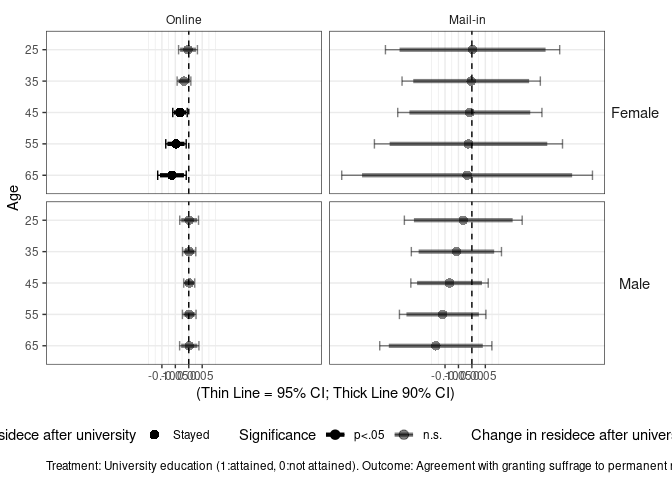
\includegraphics{analysis_1x_original_mail_v5_files/figure-latex/unnamed-chunk-40-1.pdf}

\begin{Shaded}
\begin{Highlighting}[]
\KeywordTok{ggsave}\NormalTok{(}\KeywordTok{paste0}\NormalTok{(projdir,}\StringTok{"/out/mailineffectplotx.png"}\NormalTok{),p,}\DataTypeTok{width=}\DecValTok{8}\NormalTok{,}\DataTypeTok{height=}\DecValTok{5}\NormalTok{)}
\end{Highlighting}
\end{Shaded}

\begin{verbatim}
## Warning: position_dodge requires non-overlapping x intervals

## Warning: position_dodge requires non-overlapping x intervals

## Warning: position_dodge requires non-overlapping x intervals

## Warning: position_dodge requires non-overlapping x intervals
\end{verbatim}

\begin{Shaded}
\begin{Highlighting}[]
\CommentTok{## Multinomial Logit ##}

\NormalTok{extout <-}\StringTok{ }\ControlFlowTok{function}\NormalTok{(gender,ageset,}\DataTypeTok{sub=}\DecValTok{1}\NormalTok{) \{}
  
  \ControlFlowTok{if}\NormalTok{ (gender}\OperatorTok{==}\StringTok{"Male"}\NormalTok{) sifcct}\OperatorTok{$}\NormalTok{gender <-}\StringTok{ }\NormalTok{sifcct}\OperatorTok{$}\NormalTok{female}
  \ControlFlowTok{if}\NormalTok{ (gender}\OperatorTok{==}\StringTok{"Female"}\NormalTok{) sifcct}\OperatorTok{$}\NormalTok{gender <-}\StringTok{ }\NormalTok{sifcct}\OperatorTok{$}\NormalTok{male}
\NormalTok{  sifcct}\OperatorTok{$}\NormalTok{ageset <-}\StringTok{ }\NormalTok{(sifcct}\OperatorTok{$}\NormalTok{age }\OperatorTok{-}\StringTok{ }\NormalTok{ageset)}\OperatorTok{/}\DecValTok{10}
  
  \ControlFlowTok{if}\NormalTok{ (sub}\OperatorTok{==}\DecValTok{1}\NormalTok{) \{}
    \CommentTok{# modset <- multinom(foreignsuff3x ~ edu2 * gender * ageset + lvpr + zip_did + sqrt(c10_sreg_fper) + }
    \CommentTok{#                      I(c10_sreg_edu_ugsP/10) + didper + sqrt(c10_mun_fper) + I(c10_mun_edu_ugsP/10) + }
    \CommentTok{#                      as.factor(wave), data=sifcct[which(sifcct$age - sifcct$lvlen<=15),],}
    \CommentTok{#                    Hess = TRUE)}
\NormalTok{    sifcct.mlogit.tmp <-}\StringTok{ }\KeywordTok{dfidx}\NormalTok{(sifcct[}\KeywordTok{which}\NormalTok{(sifcct}\OperatorTok{$}\NormalTok{age }\OperatorTok{-}\StringTok{ }\NormalTok{sifcct}\OperatorTok{$}\NormalTok{lvlen}\OperatorTok{<=}\DecValTok{15}\NormalTok{),],}
                               \DataTypeTok{shape =} \StringTok{"wide"}\NormalTok{, }\DataTypeTok{choice =} \StringTok{"foreignsuff3x"}\NormalTok{)}
    \CommentTok{# levels(sifcct.mlogit.tmp$idx$id2) <- c("Disagree","Neither","Agree")}
\NormalTok{    modset <-}\StringTok{ }\KeywordTok{mlogit}\NormalTok{(foreignsuff3x }\OperatorTok{~}\StringTok{ }\DecValTok{0} \OperatorTok{|}\StringTok{ }\NormalTok{edu2 }\OperatorTok{*}\StringTok{ }\NormalTok{gender }\OperatorTok{*}\StringTok{ }\NormalTok{ageset }\OperatorTok{+}\StringTok{ }\NormalTok{lvpr }\OperatorTok{+}\StringTok{ }\NormalTok{zip_did }\OperatorTok{+}\StringTok{ }\KeywordTok{sqrt}\NormalTok{(c10_sreg_fper) }\OperatorTok{+}\StringTok{ }
\StringTok{                       }\KeywordTok{I}\NormalTok{(c10_sreg_edu_ugsP}\OperatorTok{/}\DecValTok{10}\NormalTok{) }\OperatorTok{+}\StringTok{ }\NormalTok{didper }\OperatorTok{+}\StringTok{ }\KeywordTok{sqrt}\NormalTok{(c10_mun_fper) }\OperatorTok{+}\StringTok{ }\KeywordTok{I}\NormalTok{(c10_mun_edu_ugsP}\OperatorTok{/}\DecValTok{10}\NormalTok{) }\OperatorTok{+}\StringTok{ }
\StringTok{                       }\KeywordTok{as.factor}\NormalTok{(wave), }\DataTypeTok{data=}\NormalTok{sifcct.mlogit.tmp, }\DataTypeTok{reflevel=}\StringTok{"Disagree"}\NormalTok{)}
\NormalTok{    subname =}\StringTok{ "Stayed"}
\NormalTok{  \} }\ControlFlowTok{else}\NormalTok{ \{}
    \CommentTok{# modset <- multinom(foreignsuff3x ~ edu2 * gender * ageset + lvpr + as.factor(wave), }
    \CommentTok{#                    data=sifcct[which(sifcct$age - sifcct$lvlen>=23),],}
    \CommentTok{#                    Hess = TRUE)}
\NormalTok{    sifcct.mlogit.tmp <-}\StringTok{ }\KeywordTok{dfidx}\NormalTok{(sifcct[}\KeywordTok{which}\NormalTok{(sifcct}\OperatorTok{$}\NormalTok{age }\OperatorTok{-}\StringTok{ }\NormalTok{sifcct}\OperatorTok{$}\NormalTok{lvlen}\OperatorTok{>=}\DecValTok{23}\NormalTok{),],}
                               \DataTypeTok{shape =} \StringTok{"wide"}\NormalTok{, }\DataTypeTok{choice =} \StringTok{"foreignsuff3x"}\NormalTok{)}
    \CommentTok{# levels(sifcct.mlogit.tmp$idx$id2) <- c("Disagree","Neither","Agree")}
\NormalTok{    modset <-}\StringTok{ }\KeywordTok{mlogit}\NormalTok{(foreignsuff3x }\OperatorTok{~}\StringTok{ }\DecValTok{0} \OperatorTok{|}\StringTok{ }\NormalTok{edu2 }\OperatorTok{*}\StringTok{ }\NormalTok{gender }\OperatorTok{*}\StringTok{ }\NormalTok{ageset }\OperatorTok{+}\StringTok{ }\NormalTok{lvpr }\OperatorTok{+}\StringTok{ }\KeywordTok{as.factor}\NormalTok{(wave), }
                     \DataTypeTok{data=}\NormalTok{sifcct.mlogit.tmp, }\DataTypeTok{reflevel=}\StringTok{"Disagree"}\NormalTok{)}
\NormalTok{    subname =}\StringTok{ "Moved"}
\NormalTok{  \}}
  
  \CommentTok{# modres <- extract(modset)}
  
  \CommentTok{# res <- c(gender,ageset,modres@coef[grep("^Agree: edu2$",modres@coef.names)],}
  \CommentTok{#          modres@coef[grep("^Agree: edu2$",modres@coef.names)] - qnorm(0.975)*modres@se[grep("^Agree: edu2$",modres@coef.names)],}
  \CommentTok{#          modres@coef[grep("^Agree: edu2$",modres@coef.names)] + qnorm(0.975)*modres@se[grep("^Agree: edu2$",modres@coef.names)],}
  \CommentTok{#          modres@coef[grep("^Agree: edu2$",modres@coef.names)] - qnorm(0.95)*modres@se[grep("^Agree: edu2$",modres@coef.names)],}
  \CommentTok{#          modres@coef[grep("^Agree: edu2$",modres@coef.names)] + qnorm(0.95)*modres@se[grep("^Agree: edu2$",modres@coef.names)],}
  \CommentTok{#          modres@se[grep("^Agree: edu2$",modres@coef.names)],}
  \CommentTok{#          modres@pvalues[grep("^Agree: edu2$",modres@coef.names)],}
  \CommentTok{#          subname)}
\NormalTok{  res <-}\StringTok{ }\KeywordTok{c}\NormalTok{(gender,ageset,}\KeywordTok{coef}\NormalTok{(modset)[}\DecValTok{3}\NormalTok{],}
           \KeywordTok{coefci}\NormalTok{(modset, }\DataTypeTok{vcov=}\NormalTok{sandwich, }\DataTypeTok{level =} \FloatTok{0.95}\NormalTok{)[}\DecValTok{3}\NormalTok{,],}
           \KeywordTok{coefci}\NormalTok{(modset, }\DataTypeTok{vcov=}\NormalTok{sandwich, }\DataTypeTok{level =} \FloatTok{0.90}\NormalTok{)[}\DecValTok{3}\NormalTok{,],}
           \KeywordTok{coeftest}\NormalTok{(modset, }\DataTypeTok{vcov=}\NormalTok{sandwich)[}\DecValTok{3}\NormalTok{,}\KeywordTok{c}\NormalTok{(}\DecValTok{2}\NormalTok{,}\DecValTok{4}\NormalTok{)],}
\NormalTok{           subname)}
  
  \KeywordTok{names}\NormalTok{(res) <-}\StringTok{ }\KeywordTok{c}\NormalTok{(}\StringTok{"gender"}\NormalTok{,}\StringTok{"age"}\NormalTok{,}\StringTok{"est"}\NormalTok{,}\StringTok{"lci95"}\NormalTok{,}\StringTok{"uci95"}\NormalTok{,}\StringTok{"lci90"}\NormalTok{,}\StringTok{"uci90"}\NormalTok{,}\StringTok{"se"}\NormalTok{,}\StringTok{"p"}\NormalTok{,}\StringTok{"lv"}\NormalTok{)}
  
  \KeywordTok{return}\NormalTok{(res)}
  
\NormalTok{\}}

\NormalTok{outdt0 <-}\StringTok{ }\KeywordTok{rbind}\NormalTok{(}\KeywordTok{extout}\NormalTok{(}\StringTok{"Female"}\NormalTok{,}\DecValTok{25}\NormalTok{,}\DecValTok{2}\NormalTok{),}
                \KeywordTok{extout}\NormalTok{(}\StringTok{"Female"}\NormalTok{,}\DecValTok{35}\NormalTok{,}\DecValTok{2}\NormalTok{),}
                \KeywordTok{extout}\NormalTok{(}\StringTok{"Female"}\NormalTok{,}\DecValTok{45}\NormalTok{,}\DecValTok{2}\NormalTok{),}
                \KeywordTok{extout}\NormalTok{(}\StringTok{"Female"}\NormalTok{,}\DecValTok{55}\NormalTok{,}\DecValTok{2}\NormalTok{),}
                \KeywordTok{extout}\NormalTok{(}\StringTok{"Female"}\NormalTok{,}\DecValTok{65}\NormalTok{,}\DecValTok{2}\NormalTok{),}
                \KeywordTok{extout}\NormalTok{(}\StringTok{"Male"}\NormalTok{,}\DecValTok{25}\NormalTok{,}\DecValTok{2}\NormalTok{),}
                \KeywordTok{extout}\NormalTok{(}\StringTok{"Male"}\NormalTok{,}\DecValTok{35}\NormalTok{,}\DecValTok{2}\NormalTok{),}
                \KeywordTok{extout}\NormalTok{(}\StringTok{"Male"}\NormalTok{,}\DecValTok{45}\NormalTok{,}\DecValTok{2}\NormalTok{),}
                \KeywordTok{extout}\NormalTok{(}\StringTok{"Male"}\NormalTok{,}\DecValTok{55}\NormalTok{,}\DecValTok{2}\NormalTok{),}
                \KeywordTok{extout}\NormalTok{(}\StringTok{"Male"}\NormalTok{,}\DecValTok{65}\NormalTok{,}\DecValTok{2}\NormalTok{))}
\NormalTok{outdt0 <-}\StringTok{ }\KeywordTok{as.data.frame}\NormalTok{(outdt0)}
\ControlFlowTok{for}\NormalTok{(i }\ControlFlowTok{in} \DecValTok{2}\OperatorTok{:}\DecValTok{9}\NormalTok{) outdt0[,i] <-}\StringTok{ }\KeywordTok{as.numeric}\NormalTok{(outdt0[,i])}
\NormalTok{outdt0}\OperatorTok{$}\NormalTok{gender <-}\StringTok{ }\KeywordTok{factor}\NormalTok{(outdt0}\OperatorTok{$}\NormalTok{gender, }\DataTypeTok{levels=}\KeywordTok{unique}\NormalTok{(outdt0}\OperatorTok{$}\NormalTok{gender))}
\KeywordTok{summary}\NormalTok{(outdt0)}
\end{Highlighting}
\end{Shaded}

\begin{verbatim}
##     gender       age          est                lci95              uci95               lci90         
##  Female:5   Min.   :25   Min.   :-0.243140   Min.   :-0.47155   Min.   :-0.021194   Min.   :-0.43483  
##  Male  :5   1st Qu.:35   1st Qu.:-0.166098   1st Qu.:-0.31315   1st Qu.:-0.005643   1st Qu.:-0.28920  
##             Median :45   Median :-0.073352   Median :-0.18847   Median : 0.042493   Median :-0.17057  
##             Mean   :45   Mean   :-0.056795   Mean   :-0.20097   Mean   : 0.087382   Mean   :-0.17779  
##             3rd Qu.:55   3rd Qu.: 0.005561   3rd Qu.:-0.10201   3rd Qu.: 0.129604   3rd Qu.:-0.08472  
##             Max.   :65   Max.   : 0.195778   Max.   : 0.02856   Max.   : 0.363000   Max.   : 0.05544  
##      uci90                se                p                lv           
##  Min.   :-0.05145   Min.   :0.04746   Min.   :0.02175   Length:10         
##  1st Qu.:-0.02656   1st Qu.:0.05482   1st Qu.:0.02910   Class :character  
##  Median : 0.02387   Median :0.06967   Median :0.07742   Mode  :character  
##  Mean   : 0.06420   Mean   :0.07356   Mean   :0.25585                     
##  3rd Qu.: 0.10943   3rd Qu.:0.08443   3rd Qu.:0.21760                     
##  Max.   : 0.33611   Max.   :0.11653   Max.   :0.96055
\end{verbatim}

\begin{Shaded}
\begin{Highlighting}[]
\NormalTok{extout <-}\StringTok{ }\ControlFlowTok{function}\NormalTok{(gender,ageset,}\DataTypeTok{sub=}\DecValTok{1}\NormalTok{) \{}
  
  \ControlFlowTok{if}\NormalTok{ (gender}\OperatorTok{==}\StringTok{"Male"}\NormalTok{) mail}\OperatorTok{$}\NormalTok{gender <-}\StringTok{ }\NormalTok{mail}\OperatorTok{$}\NormalTok{female}
  \ControlFlowTok{if}\NormalTok{ (gender}\OperatorTok{==}\StringTok{"Female"}\NormalTok{) mail}\OperatorTok{$}\NormalTok{gender <-}\StringTok{ }\NormalTok{mail}\OperatorTok{$}\NormalTok{male}
\NormalTok{  mail}\OperatorTok{$}\NormalTok{ageset <-}\StringTok{ }\NormalTok{(mail}\OperatorTok{$}\NormalTok{age }\OperatorTok{-}\StringTok{ }\NormalTok{ageset)}\OperatorTok{/}\DecValTok{10}
  
  \ControlFlowTok{if}\NormalTok{ (sub}\OperatorTok{==}\DecValTok{1}\NormalTok{) \{}
    \CommentTok{# modset <- multinom(foreignsuff3x ~ edu2 * gender * ageset + lvpr + zip_did + sqrt(c10_sreg_fper) +}
    \CommentTok{#                      I(c10_sreg_edu_ugsP/10) + didper + sqrt(c10_mun_fper) + I(c10_mun_edu_ugsP/10),}
    \CommentTok{#                    data=mail[which(mail$age - mail$lvlen<=15),],}
    \CommentTok{#                    Hess = TRUE)}
\NormalTok{    mail.mlogit.tmp <-}\StringTok{ }\KeywordTok{dfidx}\NormalTok{(mail[}\KeywordTok{which}\NormalTok{(mail}\OperatorTok{$}\NormalTok{age }\OperatorTok{-}\StringTok{ }\NormalTok{mail}\OperatorTok{$}\NormalTok{lvlen}\OperatorTok{<=}\DecValTok{15}\NormalTok{),],}
                             \DataTypeTok{shape =} \StringTok{"wide"}\NormalTok{, }\DataTypeTok{choice =} \StringTok{"foreignsuff3x"}\NormalTok{)}
    \CommentTok{# levels(mail.mlogit.tmp$idx$id2) <- c("Disagree","Neither","Agree")}
\NormalTok{    modset <-}\StringTok{ }\KeywordTok{mlogit}\NormalTok{(foreignsuff3x }\OperatorTok{~}\StringTok{ }\DecValTok{0} \OperatorTok{|}\StringTok{ }\NormalTok{edu2 }\OperatorTok{*}\StringTok{ }\NormalTok{gender }\OperatorTok{*}\StringTok{ }\NormalTok{ageset }\OperatorTok{+}\StringTok{ }\NormalTok{lvpr }\OperatorTok{+}\StringTok{ }\NormalTok{zip_did }\OperatorTok{+}\StringTok{ }\KeywordTok{sqrt}\NormalTok{(c10_sreg_fper) }\OperatorTok{+}\StringTok{ }
\StringTok{                       }\KeywordTok{I}\NormalTok{(c10_sreg_edu_ugsP}\OperatorTok{/}\DecValTok{10}\NormalTok{) }\OperatorTok{+}\StringTok{ }\NormalTok{didper }\OperatorTok{+}\StringTok{ }\KeywordTok{sqrt}\NormalTok{(c10_mun_fper) }\OperatorTok{+}\StringTok{ }\KeywordTok{I}\NormalTok{(c10_mun_edu_ugsP}\OperatorTok{/}\DecValTok{10}\NormalTok{), }
                     \DataTypeTok{data=}\NormalTok{mail.mlogit.tmp, }\DataTypeTok{reflevel=}\StringTok{"Disagree"}\NormalTok{)}
\NormalTok{    subname =}\StringTok{ "Stayed"}
\NormalTok{  \} }\ControlFlowTok{else}\NormalTok{ \{}
    \CommentTok{# modset <- multinom(foreignsuff3x ~ edu2 * gender * ageset + lvpr, }
    \CommentTok{#                    data=mail[which(mail$age - mail$lvlen>=23),],}
    \CommentTok{#                    Hess = TRUE)}
\NormalTok{    mail.mlogit.tmp <-}\StringTok{ }\KeywordTok{dfidx}\NormalTok{(mail[}\KeywordTok{which}\NormalTok{(mail}\OperatorTok{$}\NormalTok{age }\OperatorTok{-}\StringTok{ }\NormalTok{mail}\OperatorTok{$}\NormalTok{lvlen}\OperatorTok{>=}\DecValTok{23}\NormalTok{),],}
                             \DataTypeTok{shape =} \StringTok{"wide"}\NormalTok{, }\DataTypeTok{choice =} \StringTok{"foreignsuff3x"}\NormalTok{)}
    \CommentTok{# levels(mail.mlogit.tmp$idx$id2) <- c("Disagree","Neither","Agree")}
\NormalTok{    modset <-}\StringTok{ }\KeywordTok{mlogit}\NormalTok{(foreignsuff3x }\OperatorTok{~}\StringTok{ }\DecValTok{0} \OperatorTok{|}\StringTok{ }\NormalTok{edu2 }\OperatorTok{*}\StringTok{ }\NormalTok{gender }\OperatorTok{*}\StringTok{ }\NormalTok{ageset }\OperatorTok{+}\StringTok{ }\NormalTok{lvpr, }
                     \DataTypeTok{data=}\NormalTok{mail.mlogit.tmp, }\DataTypeTok{reflevel=}\StringTok{"Disagree"}\NormalTok{)}
\NormalTok{    subname =}\StringTok{ "Moved"}
\NormalTok{  \}}
  
  \CommentTok{# modres <- extract(modset)}
  
  \CommentTok{# res <- c(gender,ageset,modres@coef[grep("^Agree: edu2$",modres@coef.names)],}
  \CommentTok{#          modres@coef[grep("^Agree: edu2$",modres@coef.names)] - qnorm(0.975)*modres@se[grep("^Agree: edu2$",modres@coef.names)],}
  \CommentTok{#          modres@coef[grep("^Agree: edu2$",modres@coef.names)] + qnorm(0.975)*modres@se[grep("^Agree: edu2$",modres@coef.names)],}
  \CommentTok{#          modres@coef[grep("^Agree: edu2$",modres@coef.names)] - qnorm(0.95)*modres@se[grep("^Agree: edu2$",modres@coef.names)],}
  \CommentTok{#          modres@coef[grep("^Agree: edu2$",modres@coef.names)] + qnorm(0.95)*modres@se[grep("^Agree: edu2$",modres@coef.names)],}
  \CommentTok{#          modres@se[grep("^Agree: edu2$",modres@coef.names)],}
  \CommentTok{#          modres@pvalues[grep("^Agree: edu2$",modres@coef.names)],}
  \CommentTok{#          subname)}
\NormalTok{  res <-}\StringTok{ }\KeywordTok{c}\NormalTok{(gender,ageset,}\KeywordTok{coef}\NormalTok{(modset)[}\DecValTok{3}\NormalTok{],}
           \KeywordTok{coefci}\NormalTok{(modset, }\DataTypeTok{vcov=}\NormalTok{sandwich, }\DataTypeTok{level =} \FloatTok{0.95}\NormalTok{)[}\DecValTok{3}\NormalTok{,],}
           \KeywordTok{coefci}\NormalTok{(modset, }\DataTypeTok{vcov=}\NormalTok{sandwich, }\DataTypeTok{level =} \FloatTok{0.90}\NormalTok{)[}\DecValTok{3}\NormalTok{,],}
           \KeywordTok{coeftest}\NormalTok{(modset, }\DataTypeTok{vcov=}\NormalTok{sandwich)[}\DecValTok{3}\NormalTok{,}\KeywordTok{c}\NormalTok{(}\DecValTok{2}\NormalTok{,}\DecValTok{4}\NormalTok{)],}
\NormalTok{           subname)}
  
  \KeywordTok{names}\NormalTok{(res) <-}\StringTok{ }\KeywordTok{c}\NormalTok{(}\StringTok{"gender"}\NormalTok{,}\StringTok{"age"}\NormalTok{,}\StringTok{"est"}\NormalTok{,}\StringTok{"lci95"}\NormalTok{,}\StringTok{"uci95"}\NormalTok{,}\StringTok{"lci90"}\NormalTok{,}\StringTok{"uci90"}\NormalTok{,}\StringTok{"se"}\NormalTok{,}\StringTok{"p"}\NormalTok{,}\StringTok{"lv"}\NormalTok{)}
  
  \KeywordTok{return}\NormalTok{(res)}
  
\NormalTok{\}}

\NormalTok{outdtm <-}\StringTok{ }\KeywordTok{rbind}\NormalTok{(}\KeywordTok{extout}\NormalTok{(}\StringTok{"Female"}\NormalTok{,}\DecValTok{25}\NormalTok{,}\DecValTok{2}\NormalTok{),}
                \KeywordTok{extout}\NormalTok{(}\StringTok{"Female"}\NormalTok{,}\DecValTok{35}\NormalTok{,}\DecValTok{2}\NormalTok{),}
                \KeywordTok{extout}\NormalTok{(}\StringTok{"Female"}\NormalTok{,}\DecValTok{45}\NormalTok{,}\DecValTok{2}\NormalTok{),}
                \KeywordTok{extout}\NormalTok{(}\StringTok{"Female"}\NormalTok{,}\DecValTok{55}\NormalTok{,}\DecValTok{2}\NormalTok{),}
                \KeywordTok{extout}\NormalTok{(}\StringTok{"Female"}\NormalTok{,}\DecValTok{65}\NormalTok{,}\DecValTok{2}\NormalTok{),}
                \KeywordTok{extout}\NormalTok{(}\StringTok{"Male"}\NormalTok{,}\DecValTok{25}\NormalTok{,}\DecValTok{2}\NormalTok{),}
                \KeywordTok{extout}\NormalTok{(}\StringTok{"Male"}\NormalTok{,}\DecValTok{35}\NormalTok{,}\DecValTok{2}\NormalTok{),}
                \KeywordTok{extout}\NormalTok{(}\StringTok{"Male"}\NormalTok{,}\DecValTok{45}\NormalTok{,}\DecValTok{2}\NormalTok{),}
                \KeywordTok{extout}\NormalTok{(}\StringTok{"Male"}\NormalTok{,}\DecValTok{55}\NormalTok{,}\DecValTok{2}\NormalTok{),}
                \KeywordTok{extout}\NormalTok{(}\StringTok{"Male"}\NormalTok{,}\DecValTok{65}\NormalTok{,}\DecValTok{2}\NormalTok{))}
\NormalTok{outdtm <-}\StringTok{ }\KeywordTok{as.data.frame}\NormalTok{(outdtm)}
\ControlFlowTok{for}\NormalTok{(i }\ControlFlowTok{in} \DecValTok{2}\OperatorTok{:}\DecValTok{9}\NormalTok{) outdtm[,i] <-}\StringTok{ }\KeywordTok{as.numeric}\NormalTok{(outdtm[,i])}
\NormalTok{outdtm}\OperatorTok{$}\NormalTok{gender <-}\StringTok{ }\KeywordTok{factor}\NormalTok{(outdtm}\OperatorTok{$}\NormalTok{gender, }\DataTypeTok{levels=}\KeywordTok{unique}\NormalTok{(outdtm}\OperatorTok{$}\NormalTok{gender))}
\KeywordTok{summary}\NormalTok{(outdtm)}
\end{Highlighting}
\end{Shaded}

\begin{verbatim}
##     gender       age          est              lci95             uci95            lci90             uci90       
##  Female:5   Min.   :25   Min.   :-0.5361   Min.   :-1.6288   Min.   :0.4162   Min.   :-1.4527   Min.   :0.3242  
##  Male  :5   1st Qu.:35   1st Qu.:-0.2346   1st Qu.:-1.1317   1st Qu.:0.4844   1st Qu.:-0.9994   1st Qu.:0.3763  
##             Median :45   Median :-0.1611   Median :-0.8692   Median :0.5341   Median :-0.7501   Median :0.4170  
##             Mean   :45   Mean   :-0.1611   Mean   :-0.9312   Mean   :0.6090   Mean   :-0.8071   Mean   :0.4849  
##             3rd Qu.:55   3rd Qu.:-0.1011   3rd Qu.:-0.7336   3rd Qu.:0.7215   3rd Qu.:-0.6393   3rd Qu.:0.5859  
##             Max.   :65   Max.   : 0.2274   Max.   :-0.3632   Max.   :0.9438   Max.   :-0.2681   Max.   :0.7524  
##        se               p               lv           
##  Min.   :0.2420   Min.   :0.3358   Length:10         
##  1st Qu.:0.3059   1st Qu.:0.4864   Class :character  
##  Median :0.3698   Median :0.6264   Mode  :character  
##  Mean   :0.3922   Mean   :0.6117                     
##  3rd Qu.:0.4382   3rd Qu.:0.6866                     
##  Max.   :0.6051   Max.   :0.8801
\end{verbatim}

\begin{Shaded}
\begin{Highlighting}[]
\NormalTok{outdt0}\OperatorTok{$}\NormalTok{data <-}\StringTok{ "Online"}
\NormalTok{outdtm}\OperatorTok{$}\NormalTok{data <-}\StringTok{ "Mail-in"}

\NormalTok{visdt <-}\StringTok{ }\KeywordTok{rbind}\NormalTok{(outdt0,outdtm)}
\NormalTok{visdt}\OperatorTok{$}\NormalTok{data <-}\StringTok{ }\KeywordTok{factor}\NormalTok{(visdt}\OperatorTok{$}\NormalTok{data, }\DataTypeTok{levels=}\KeywordTok{c}\NormalTok{(}\StringTok{"Online"}\NormalTok{,}\StringTok{"Mail-in"}\NormalTok{))}

\NormalTok{visdt}\OperatorTok{$}\NormalTok{pstar <-}\StringTok{ }\KeywordTok{factor}\NormalTok{(}\KeywordTok{ifelse}\NormalTok{(visdt}\OperatorTok{$}\NormalTok{p}\OperatorTok{>=}\NormalTok{.}\DecValTok{1}\NormalTok{,}\StringTok{"n.s."}\NormalTok{,}\KeywordTok{ifelse}\NormalTok{(visdt}\OperatorTok{$}\NormalTok{p}\OperatorTok{>=}\NormalTok{.}\DecValTok{05}\NormalTok{,}\StringTok{"p<.1"}\NormalTok{,}\StringTok{"p<.05"}\NormalTok{)),}
                      \DataTypeTok{levels =} \KeywordTok{c}\NormalTok{(}\StringTok{"p<.05"}\NormalTok{,}\StringTok{"p<.1"}\NormalTok{,}\StringTok{"n.s."}\NormalTok{))}

\KeywordTok{saveRDS}\NormalTok{(}\KeywordTok{subset}\NormalTok{(visdt, data}\OperatorTok{==}\StringTok{"Mail-in"}\NormalTok{), }\KeywordTok{paste0}\NormalTok{(projdir, }\StringTok{"/out/visdtx_mail_multinom.rds"}\NormalTok{))}

\KeywordTok{require}\NormalTok{(ggplot2)}
\NormalTok{p <-}\StringTok{ }\KeywordTok{ggplot}\NormalTok{(visdt, }\KeywordTok{aes}\NormalTok{(}\DataTypeTok{x=}\KeywordTok{factor}\NormalTok{(age, }\DataTypeTok{levels=}\KeywordTok{rev}\NormalTok{(}\KeywordTok{names}\NormalTok{(}\KeywordTok{table}\NormalTok{(age)))), }\DataTypeTok{y=}\NormalTok{est)) }\OperatorTok{+}
\StringTok{  }\KeywordTok{geom_hline}\NormalTok{(}\KeywordTok{aes}\NormalTok{(}\DataTypeTok{yintercept=}\DecValTok{0}\NormalTok{), }\DataTypeTok{linetype=}\DecValTok{2}\NormalTok{) }\OperatorTok{+}
\StringTok{  }\KeywordTok{geom_errorbar}\NormalTok{(}\KeywordTok{aes}\NormalTok{(}\DataTypeTok{ymin=}\NormalTok{lci95,}\DataTypeTok{ymax=}\NormalTok{uci95,}\DataTypeTok{colour=}\StringTok{"1"}\NormalTok{,}\DataTypeTok{alpha=}\NormalTok{pstar), }
                \DataTypeTok{position=}\KeywordTok{position_dodge}\NormalTok{(}\DataTypeTok{width=}\OperatorTok{-}\FloatTok{0.7}\NormalTok{), }\DataTypeTok{size=}\FloatTok{0.5}\NormalTok{, }\DataTypeTok{width=}\FloatTok{0.3}\NormalTok{) }\OperatorTok{+}
\StringTok{  }\KeywordTok{geom_errorbar}\NormalTok{(}\KeywordTok{aes}\NormalTok{(}\DataTypeTok{ymin=}\NormalTok{lci90,}\DataTypeTok{ymax=}\NormalTok{uci90,}\DataTypeTok{colour=}\StringTok{"1"}\NormalTok{,}\DataTypeTok{alpha=}\NormalTok{pstar),}
                \DataTypeTok{position=}\KeywordTok{position_dodge}\NormalTok{(}\DataTypeTok{width=}\OperatorTok{-}\FloatTok{0.7}\NormalTok{), }\DataTypeTok{size=}\FloatTok{1.5}\NormalTok{, }\DataTypeTok{width=}\FloatTok{0.0}\NormalTok{) }\OperatorTok{+}
\StringTok{  }\KeywordTok{geom_point}\NormalTok{(}\KeywordTok{aes}\NormalTok{(}\DataTypeTok{shape=}\NormalTok{lv, }\DataTypeTok{colour=}\StringTok{"1"}\NormalTok{,}\DataTypeTok{alpha=}\NormalTok{pstar),}
             \DataTypeTok{position=}\KeywordTok{position_dodge}\NormalTok{(}\DataTypeTok{width=}\OperatorTok{-}\FloatTok{0.7}\NormalTok{), }\DataTypeTok{size=}\DecValTok{3}\NormalTok{) }\OperatorTok{+}
\StringTok{  }\KeywordTok{facet_grid}\NormalTok{(gender }\OperatorTok{~}\StringTok{ }\NormalTok{data) }\OperatorTok{+}
\StringTok{  }\CommentTok{#scale_y_continuous(breaks = c(-0.1,-0.05,0.00,0.05)) + }
\StringTok{  }\KeywordTok{scale_shape_discrete}\NormalTok{(}\DataTypeTok{name=}\StringTok{"Change in residece after university"}\NormalTok{) }\OperatorTok{+}
\StringTok{  }\KeywordTok{scale_color_manual}\NormalTok{(}\DataTypeTok{name=}\StringTok{"Change in residece after university"}\NormalTok{,}\DataTypeTok{values=}\KeywordTok{rep}\NormalTok{(}\StringTok{"black"}\NormalTok{, }\DecValTok{1}\NormalTok{)) }\OperatorTok{+}
\StringTok{  }\KeywordTok{scale_alpha_manual}\NormalTok{(}\DataTypeTok{name=}\StringTok{"Significance"}\NormalTok{,}\DataTypeTok{values=}\KeywordTok{c}\NormalTok{(}\DecValTok{1}\NormalTok{,}\FloatTok{0.5}\NormalTok{,}\FloatTok{0.2}\NormalTok{)) }\OperatorTok{+}
\StringTok{  }\KeywordTok{ylab}\NormalTok{(}\StringTok{"(Thin Line = 95% CI; Thick Line 90% CI)"}\NormalTok{) }\OperatorTok{+}
\StringTok{  }\KeywordTok{xlab}\NormalTok{(}\StringTok{"Age"}\NormalTok{) }\OperatorTok{+}
\StringTok{  }\KeywordTok{labs}\NormalTok{(}\DataTypeTok{caption=}\StringTok{"Treatment: University education (1:attained, 0:not attained). Outcome: Agreement with granting suffrage to permanent residents (rescaled to 0-1)."}\NormalTok{) }\OperatorTok{+}
\StringTok{  }\KeywordTok{coord_flip}\NormalTok{() }\OperatorTok{+}\StringTok{ }\KeywordTok{theme_bw}\NormalTok{() }\OperatorTok{+}
\StringTok{  }\KeywordTok{theme}\NormalTok{(}\DataTypeTok{legend.position =} \StringTok{"bottom"}\NormalTok{,}
        \DataTypeTok{strip.text.x =} \KeywordTok{element_text}\NormalTok{(}\DataTypeTok{size=}\DecValTok{9}\NormalTok{),}
        \DataTypeTok{strip.text.y =} \KeywordTok{element_text}\NormalTok{(}\DataTypeTok{angle=}\DecValTok{0}\NormalTok{,}\DataTypeTok{size=}\DecValTok{11}\NormalTok{),}
        \DataTypeTok{strip.background =} \KeywordTok{element_rect}\NormalTok{(}\DataTypeTok{fill=}\OtherTok{NA}\NormalTok{,}\DataTypeTok{color=}\OtherTok{NA}\NormalTok{),}
        \DataTypeTok{plot.caption =} \KeywordTok{element_text}\NormalTok{(}\DataTypeTok{hjust=}\DecValTok{0}\NormalTok{),}
        \DataTypeTok{plot.subtitle =} \KeywordTok{element_text}\NormalTok{(}\DataTypeTok{hjust=}\FloatTok{0.5}\NormalTok{))}
\NormalTok{p}
\end{Highlighting}
\end{Shaded}

\begin{verbatim}
## Warning: position_dodge requires non-overlapping x intervals

## Warning: position_dodge requires non-overlapping x intervals

## Warning: position_dodge requires non-overlapping x intervals

## Warning: position_dodge requires non-overlapping x intervals
\end{verbatim}

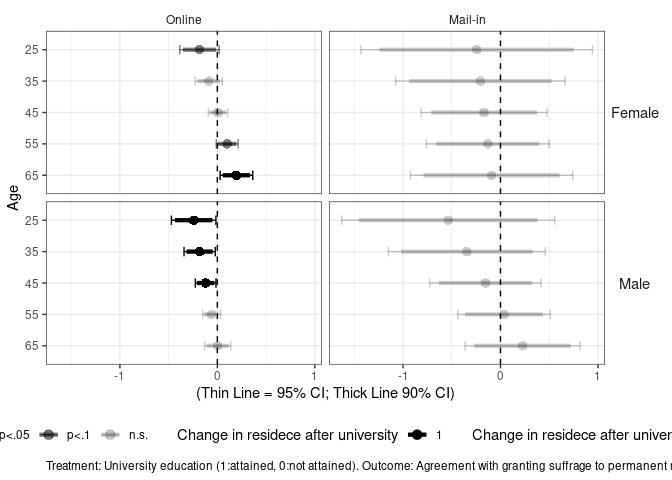
\includegraphics{analysis_1x_original_mail_v5_files/figure-latex/unnamed-chunk-40-2.pdf}

\begin{Shaded}
\begin{Highlighting}[]
\KeywordTok{ggsave}\NormalTok{(}\KeywordTok{paste0}\NormalTok{(projdir,}\StringTok{"/out/mailineffectplotx_multinom.png"}\NormalTok{),p,}\DataTypeTok{width=}\DecValTok{8}\NormalTok{,}\DataTypeTok{height=}\DecValTok{5}\NormalTok{)}
\end{Highlighting}
\end{Shaded}

\begin{verbatim}
## Warning: position_dodge requires non-overlapping x intervals

## Warning: position_dodge requires non-overlapping x intervals

## Warning: position_dodge requires non-overlapping x intervals

## Warning: position_dodge requires non-overlapping x intervals
\end{verbatim}

\hypertarget{save-image}{%
\section{Save Image}\label{save-image}}

\begin{Shaded}
\begin{Highlighting}[]
\KeywordTok{save.image}\NormalTok{(}\DataTypeTok{file=}\KeywordTok{paste0}\NormalTok{(projdir,}\StringTok{"/out/heavy/analysis_1x_original_mail_v5.RData"}\NormalTok{))}
\end{Highlighting}
\end{Shaded}

\end{document}
